%%%%%%%%%%%%%%%%%%%%%%%%%%%%%%%%%%%%%%%%%%%%%%%%%%%%%%%%%%%%%%%

% Set up document

\documentclass[xcolor={usenames,dvipsnames}]{beamer}
\usetheme{Madrid}
\setbeamersize{text margin left=5mm,text margin right=5mm}

% Dark background with non-white words: 
% \usecolortheme{owl}
% \setbeamercolor{normal text}{fg=yellow}
% \setbeamercolor{frametitle}{fg=yellow}
% \usebeamercolor[fg]{normal text}

% Used to create a section slide between section
\AtBeginSection[]{
  \begin{frame}
  \vfill
  \centering
  \begin{beamercolorbox}[sep=8pt,center,shadow=true,rounded=true]{title}
    \usebeamerfont{title}\insertsectionhead\par%
  \end{beamercolorbox}
  \vfill
  \end{frame}
}

% Remove default navigation symbols and add just  page number
\setbeamertemplate{navigation symbols}{} % Clear default navigation
% \addtobeamertemplate{navigation symbols}{}{%
%     \usebeamerfont{footline}%
%     \usebeamercolor[fg]{footline}%
%     \hspace{1em}%
%     \insertframenumber/\inserttotalframenumber
% }

% Remove from footer the names, institution, date...
% and just leave page number:
\setbeamertemplate{footline}[frame number]


% For manual font size:
\usepackage{anyfontsize}

% For smaller URLs:
\newcommand{\smallurl}[1]{\textcolor{blue}{\fontsize{4pt}{4.8pt}\selectfont \url{#1}}}


%%%%%%%%%%%%%%%%%%%%%%%%%%%%%%%%%%%%%%%%%%%%%%%%%%%%%%%%%%%%%%%

% Title page
\title{SAMuEL-2: Stroke Audit with Machine Learning 2\\Investigating variation in clinical decision-making with explainable AI}
% \subtitle{}
\author[Anna Laws]{Anna Laws, Kerry Pearn, and Michael Allen}
\institute{University of Exeter Medical School, PenCHORD}
\date{November 2022}%\today}

\begin{document}

\frame{\titlepage}

%%%%%%%%%%%%%%%%%%%%%%%%%%%%%%%%%%%%%%%%%%%%%%%%%%%%%%%%%%%%%%%


%%%%%%%%%%%%%%%%%%%%%%%%%%%%%%%%%%%%%%%%%%%%%%%%%%%%%%%%%%%%%%%

\begin{frame}
\frametitle{Who are we?}

% \begin{center}
% 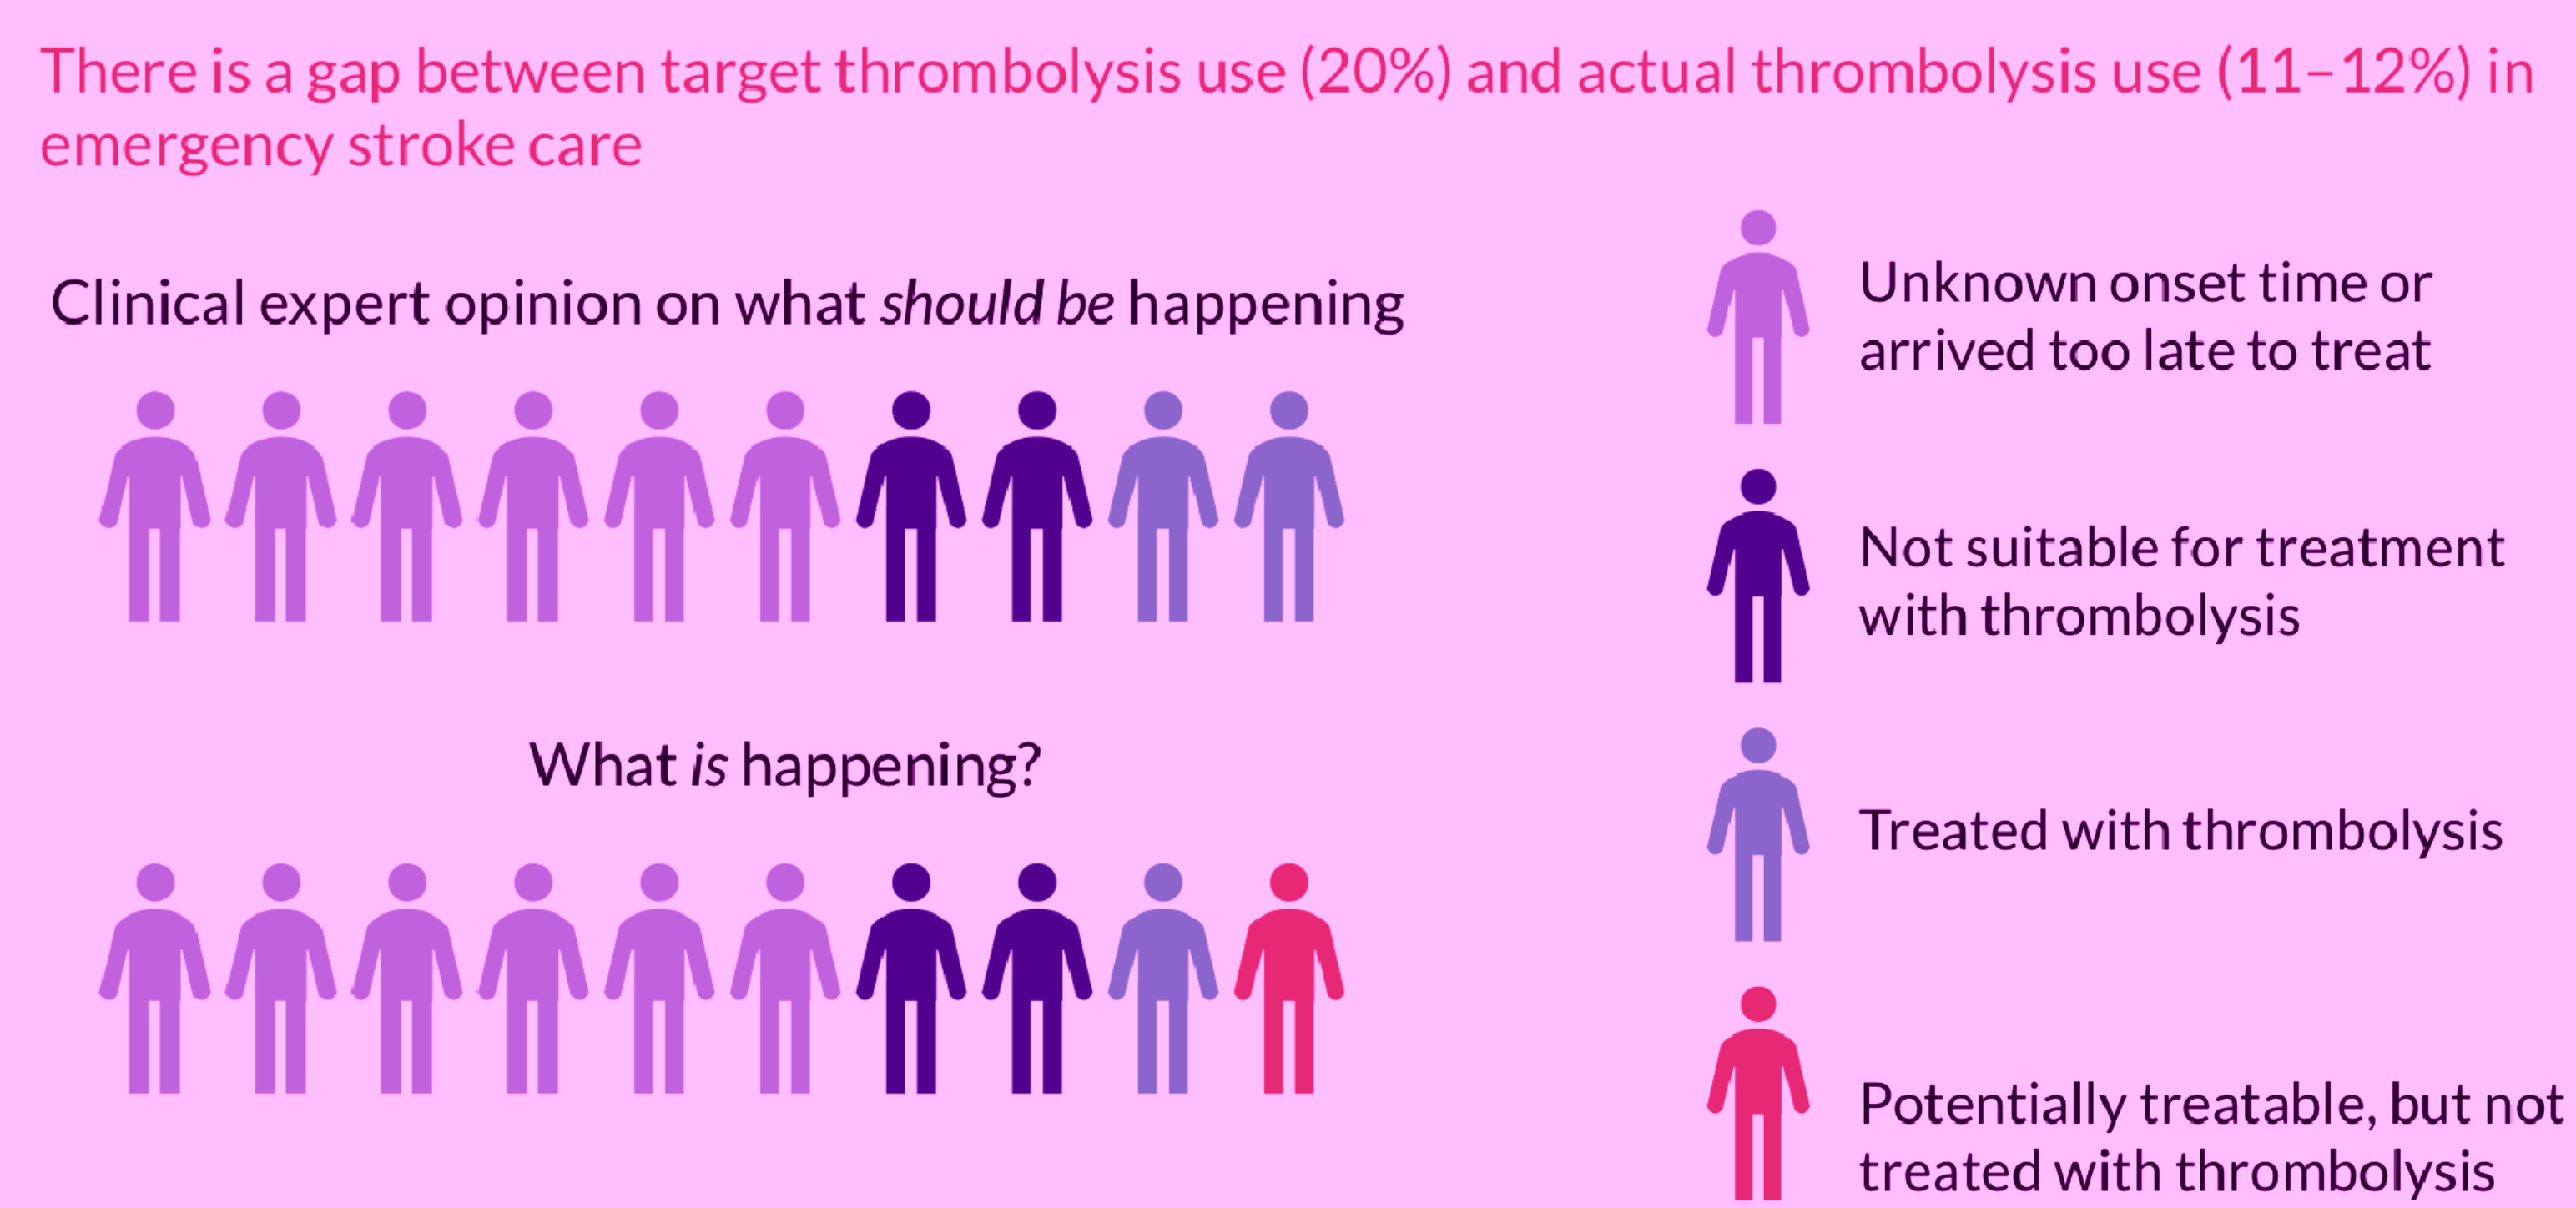
\includegraphics[width=1.0\textwidth]{./images_pink/sam_summary_pt_1}
% \end{center}

\textbf{To do - tidy me} 

Some people - quant, qual, clinician(?), PCI group... 

Explainable

FOSS 

\end{frame}



\begin{frame}
\frametitle{Outline}
\tableofcontents
\end{frame}


%%%%%%%%%%%%%%%%%%%%%%%%%%%%%%%%%%%%%%%%%%%%%%%%%%%%%%%%%%%%%%%
\section{Background}
\subsection{Treatment types} % Printed on outline slide. 

%%%%%%%%%%%%%%%%%%%%%%%%%%%%%%%%%%%%%%%%%%%%%%%%%%%%%%%%%%%%%%%


%%%%%%%%%%%%%%%%%%%%%%%%%%%%%%%%%%%%%%%%%%%%%%%%%%%%%%%%%%%%%%%

\begin{frame}
\frametitle{Two types of stroke}
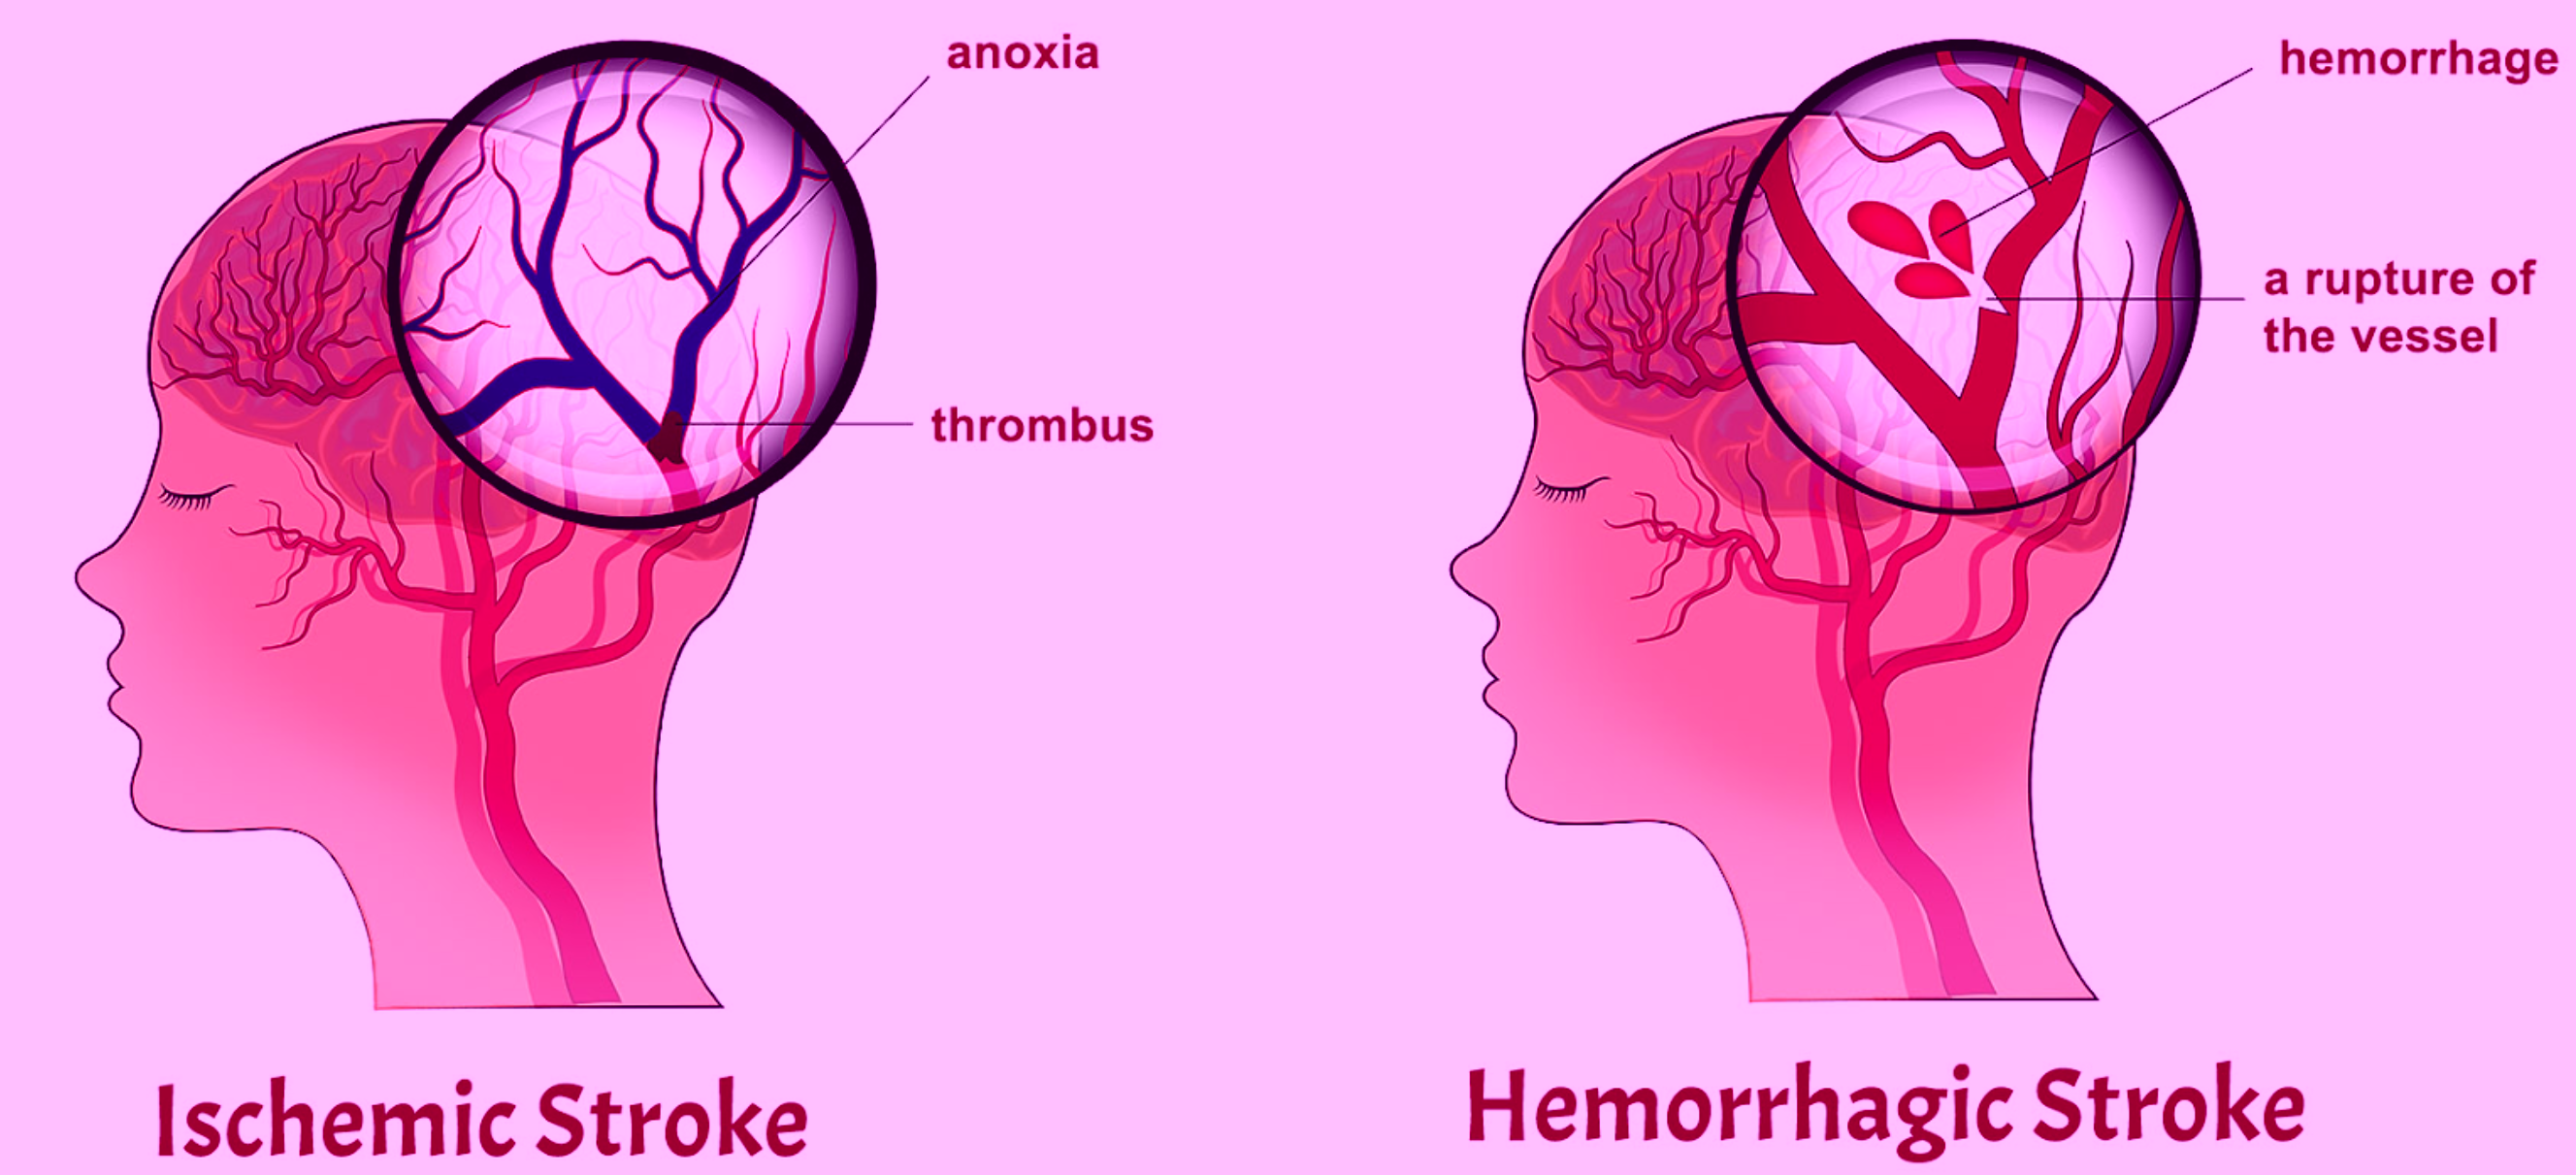
\includegraphics[width=1.0\textwidth]{./images_pink/stroke_types}
\end{frame}

%%%%%%%%%%%%%%%%%%%%%%%%%%%%%%%%%%%%%%%%%%%%%%%%%%%%%%%%%%%%%%%

\begin{frame}
\frametitle{Treatments for ischaemic stroke}

\begin{columns}
    \column{0.5\textwidth}
    \footnotesize{\textbf{Thrombolysis} aims to break down a clot by activating the body's own clot breakdown mechanisms.}
    
    \vspace{5mm}
    
    \footnotesize{Thrombolysis is given as an injection followed by an infusion (\emph{drip}).}
    
    \begin{center}
    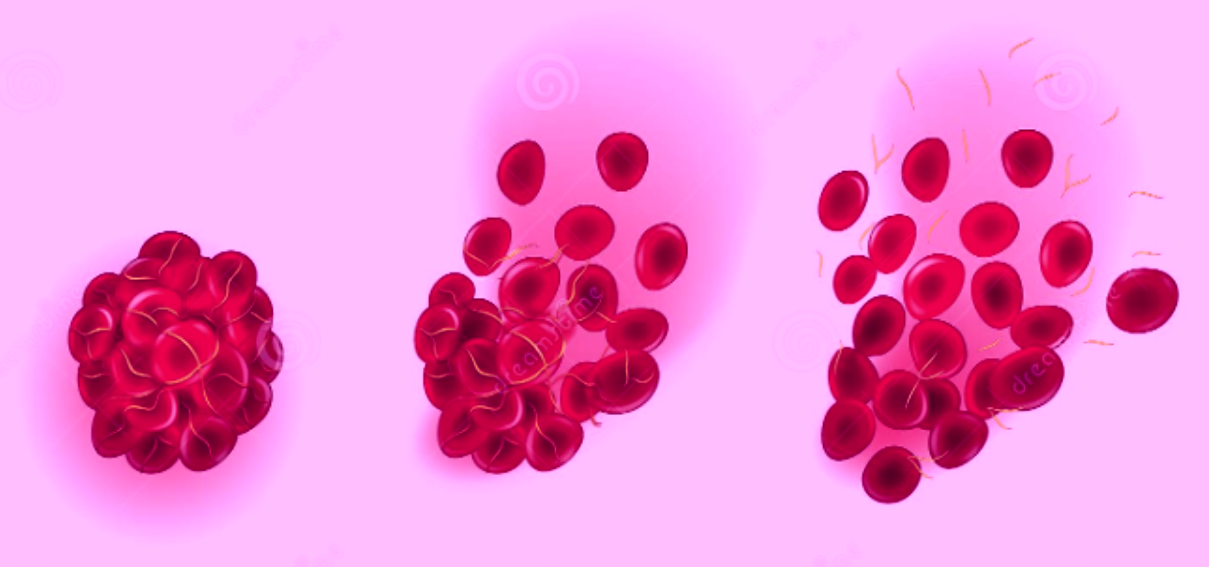
\includegraphics[width=0.6\textwidth]{./images_pink/thrombolysis_mechanism}
    \end{center}
    
    \column{0.5\textwidth}
    \footnotesize{\textbf{Thrombectomy} aims to remove the blockage.}
    
    \vspace{5mm}
    
    \footnotesize{Thrombectomy uses a mesh device that enters the blocked blood vessel and physically removes the clot.}
    
    \textbf{\textcolor{red}{To do - GET AN IMAGE}}
    
    \begin{center}
    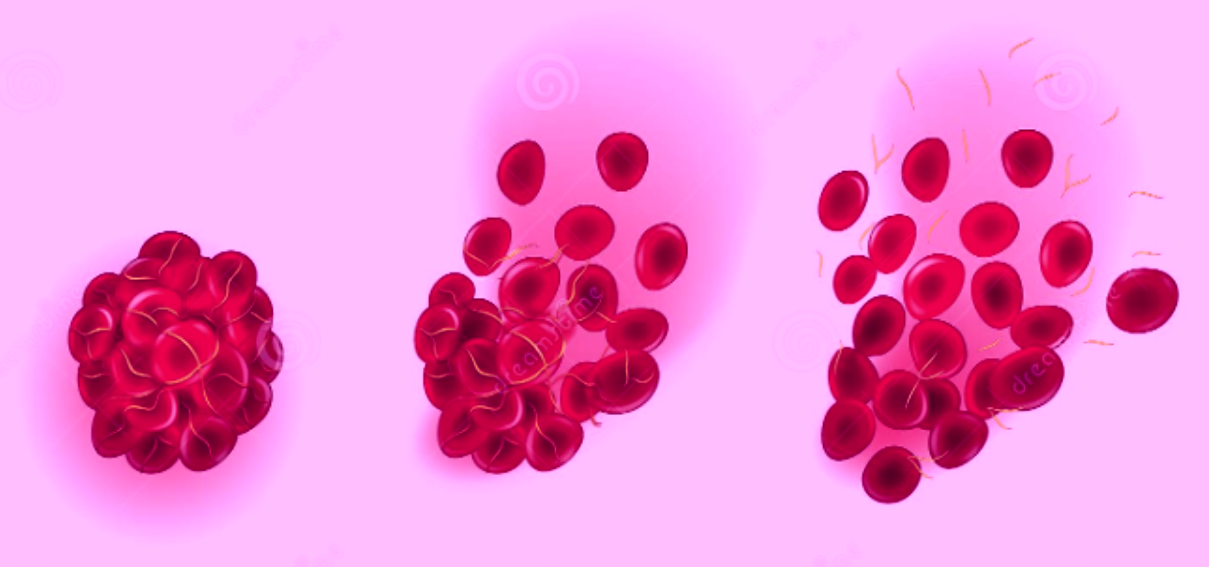
\includegraphics[width=0.6\textwidth]{./images_pink/thrombolysis_mechanism}
    \end{center}

\end{columns}

\vspace{2em}
\emph{Downsides:} not everyone is eligible for treatment, the treatments become less effective the later they are given, and there is a small chance of death. 

\end{frame}


%%%%%%%%%%%%%%%%%%%%%%%%%%%%%%%%%%%%%%%%%%%%%%%%%%%%%%%%%%%%%%%

\begin{frame}
\frametitle{What is the problem?}

\begin{center}
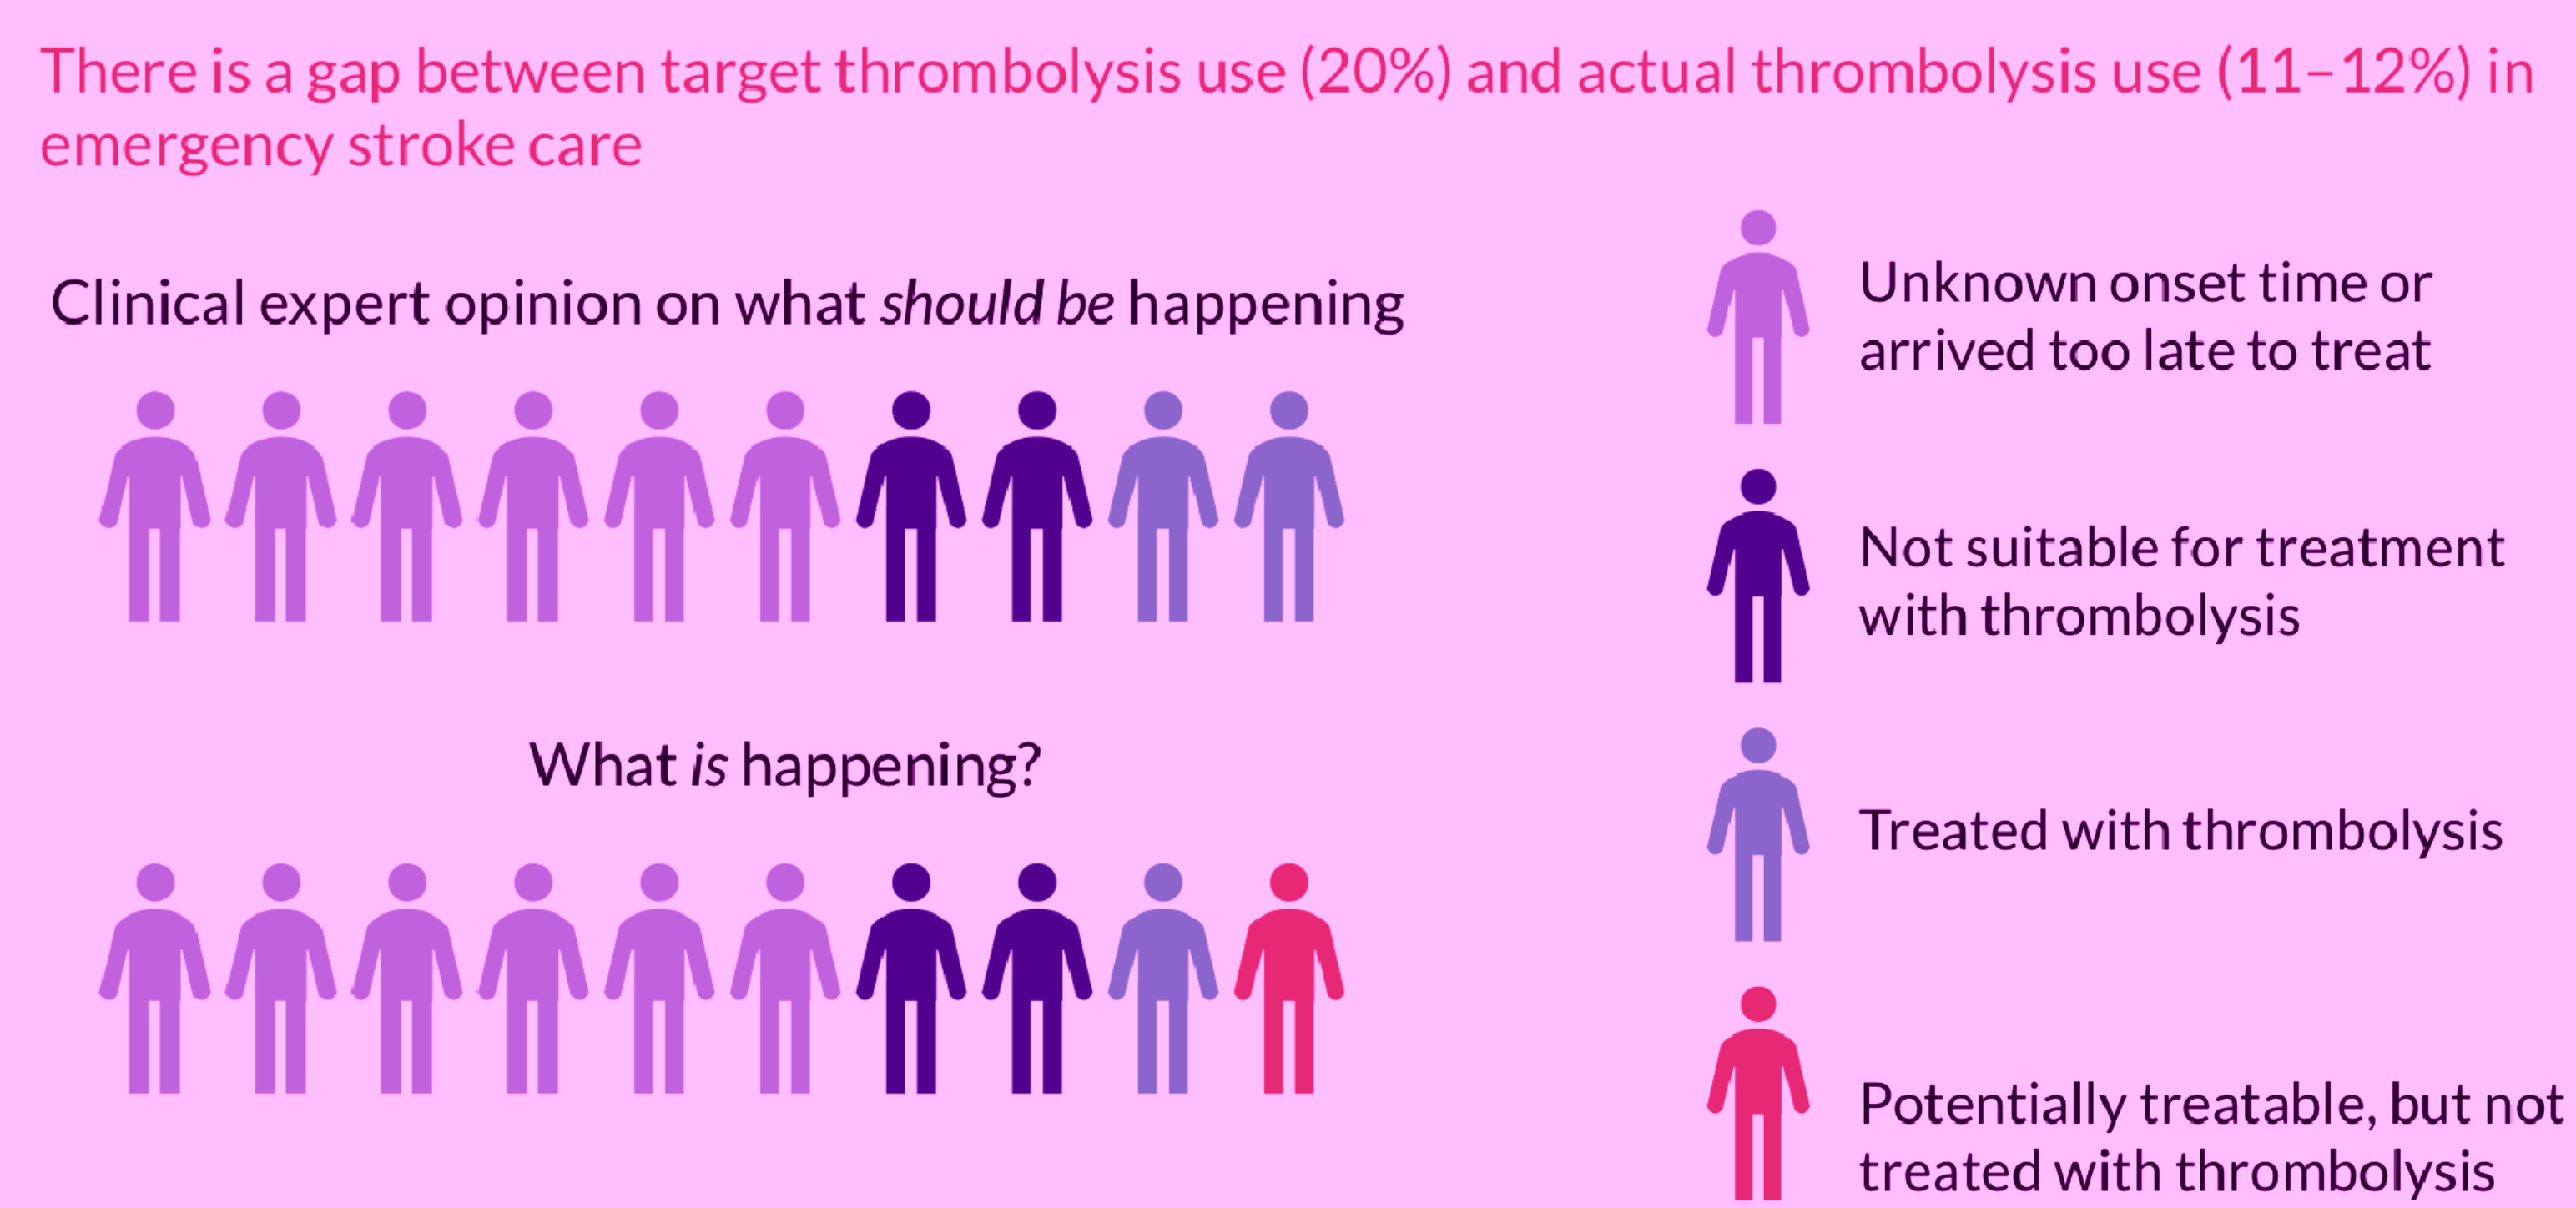
\includegraphics[width=1.0\textwidth]{./images_pink/sam_summary_pt_1}
\end{center}

 
Thrombolysis rates in England and Wales have been stable at 11-12\% for 10 years, against a NHS Long Term Plan target of 20\%.
% Thrombolysis rates at individual hospitals range from 5\% to 25\%.


% \begin{itemize}
%     \setlength\itemsep{5mm}
%     \item Expert clinical opinion is that one in five people (20\%) should be receiving thrombolysis.
%     \item In England, about 1 in 9 people (11\%) actually receive thrombolysis.
%     % \item Nearly half the people who \emph{could} benefit from thrombolysis do not currently have the opportunity.
% \end{itemize}

\end{frame}




%%%%%%%%%%%%%%%%%%%%%%%%%%%%%%%%%%%%%%%%%%%%%%%%%%%%%%%%%%%%%%%

\begin{frame}
\frametitle{Use of thrombolysis varies considerably between hospitals}
\begin{center}
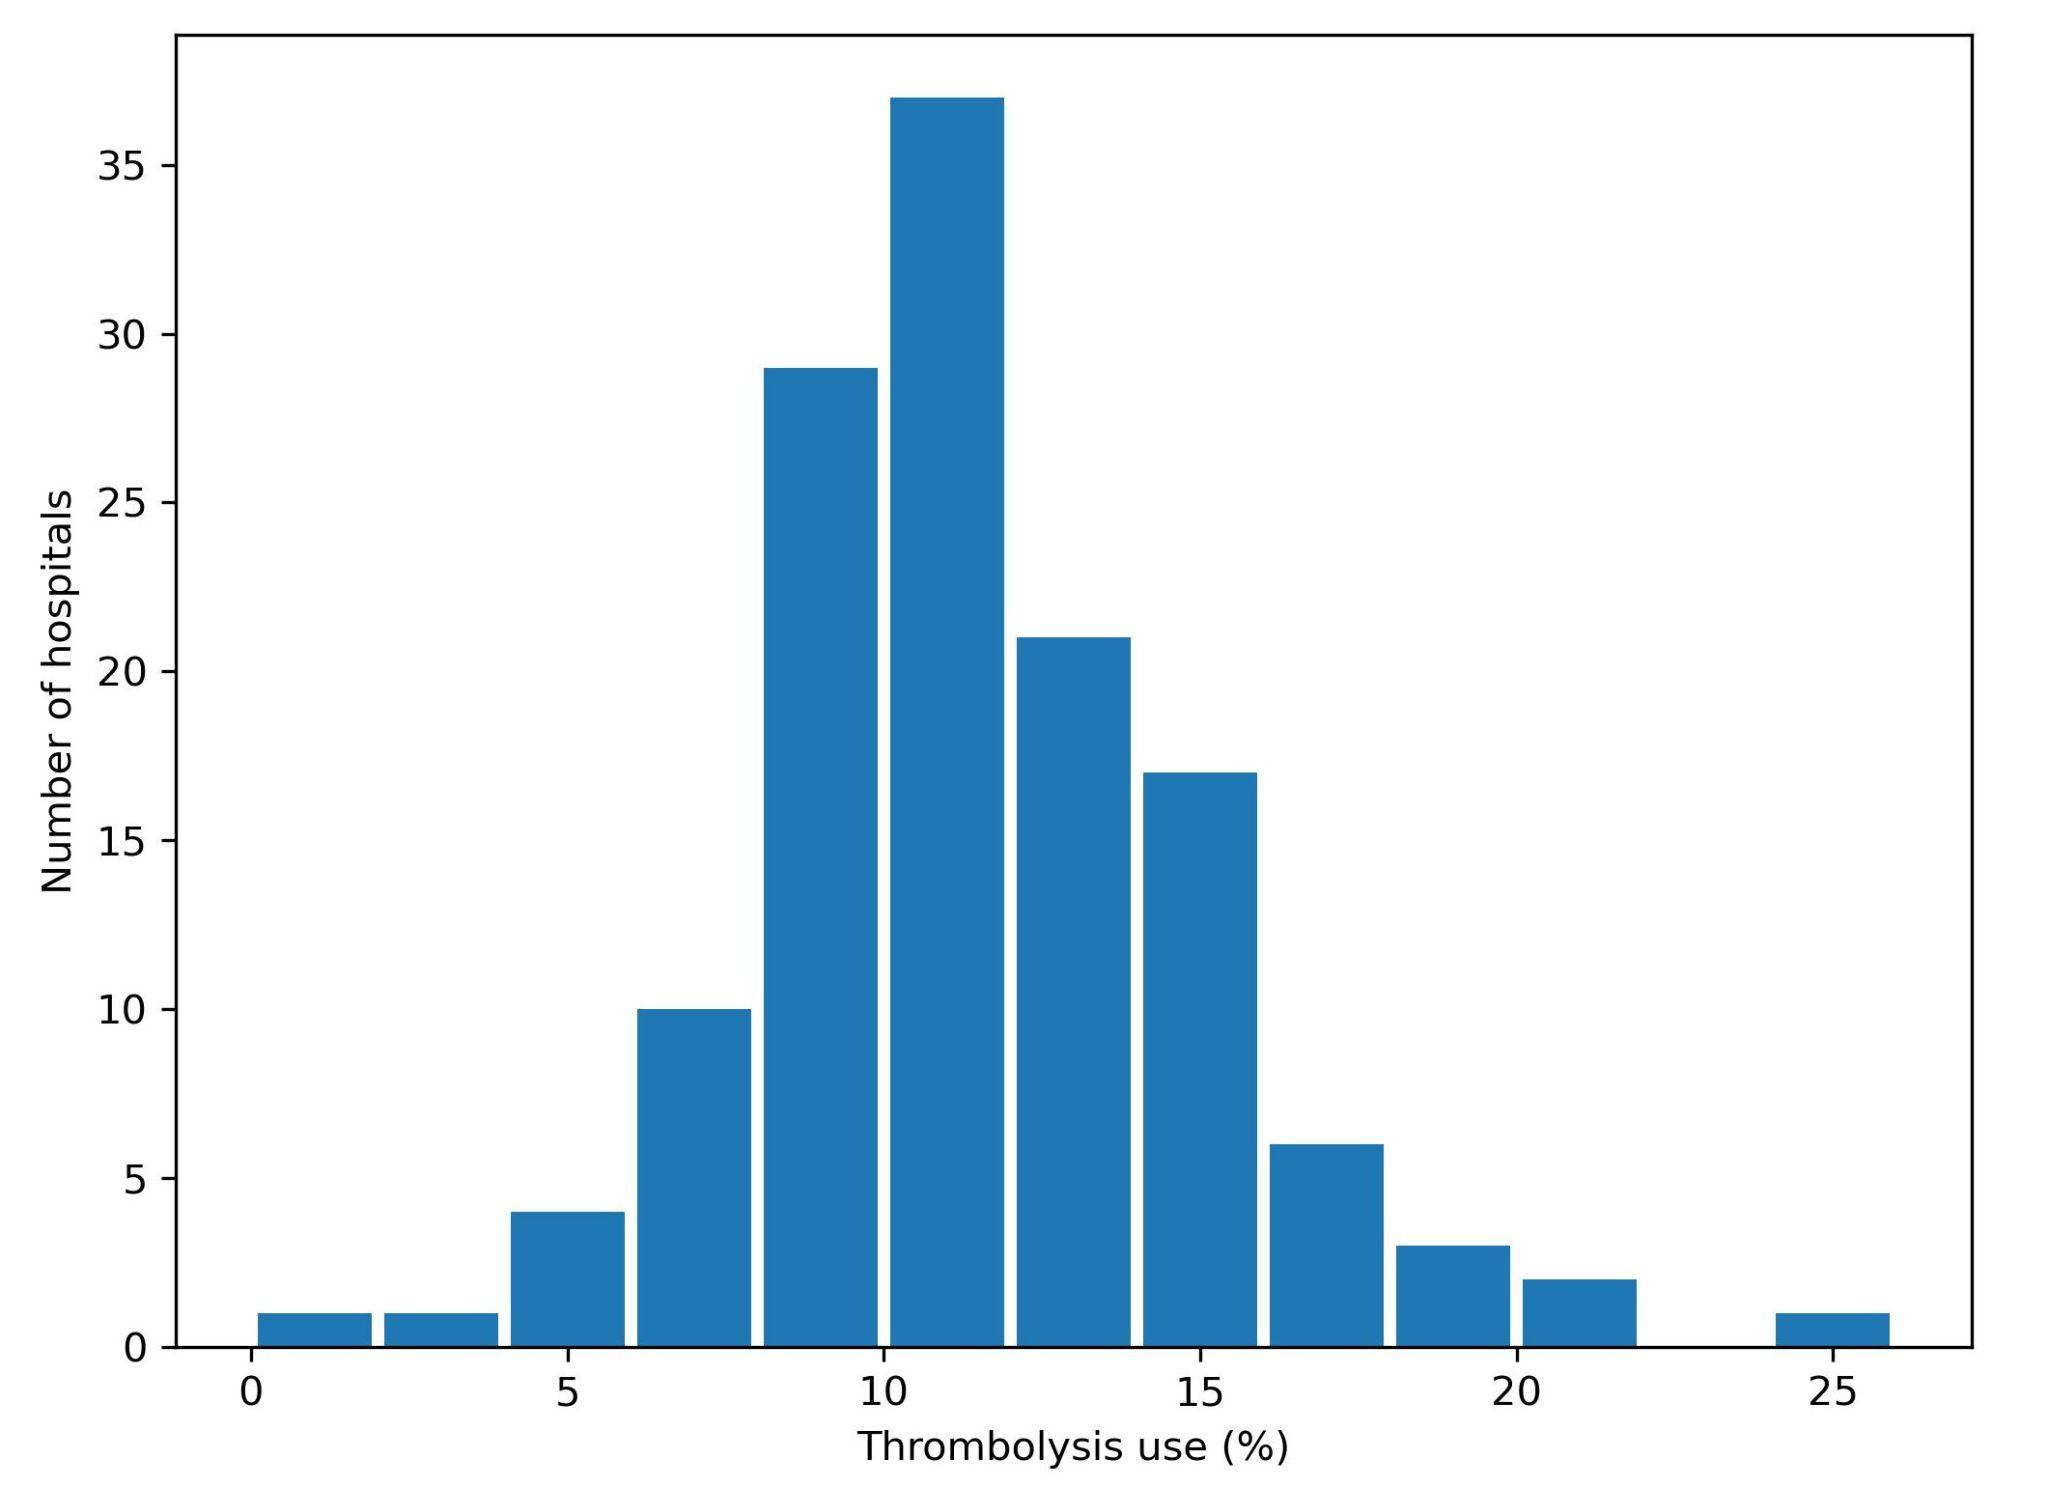
\includegraphics[width=0.6\textwidth]{./images/thrombolysis_use_between_hospitals}
\end{center}

% \vspace{-1.5em}

\footnotesize 
The single largest factor that is preventing hospitals reaching an average NHS target of 20\% thrombolysis use is clinical decision-making about which patients should receive thrombolysis.
\normalsize

\smallurl{https://samuel-book.github.io/samuel-1/pathway_sim/explained_variance_in_thrombolysis.html}

\smallurl{https://samuel-book.github.io/samuel-1/introduction/scientific_summary.html}


\end{frame}


%%%%%%%%%%%%%%%%%%%%%%%%%%%%%%%%%%%%%%%%%%%%%%%%%%%%%%%%%%%%%%%

\begin{frame}{What's the question?}

What causes this variation in thrombolysis rates, and what could reasonably be achieved at each hospital (allowing for each hospital's own patient population)?


\vspace{10mm}
\begin{quote}
  ``Your decision to treat or not treat … That’s the difficult part.\\
  That’s the grey area where everyone does a different thing.''\\
  \hfill\footnotesize\textnormal{— Stroke Consultant during interviews for SAMueL}
\end{quote}


\end{frame}


%%%%%%%%%%%%%%%%%%%%%%%%%%%%%%%%%%%%%%%%%%%%%%%%%%%%%%%%%%%%%%%

\begin{frame}
\frametitle{Breaking down the emergency stroke pathway into key steps}
\begin{center}
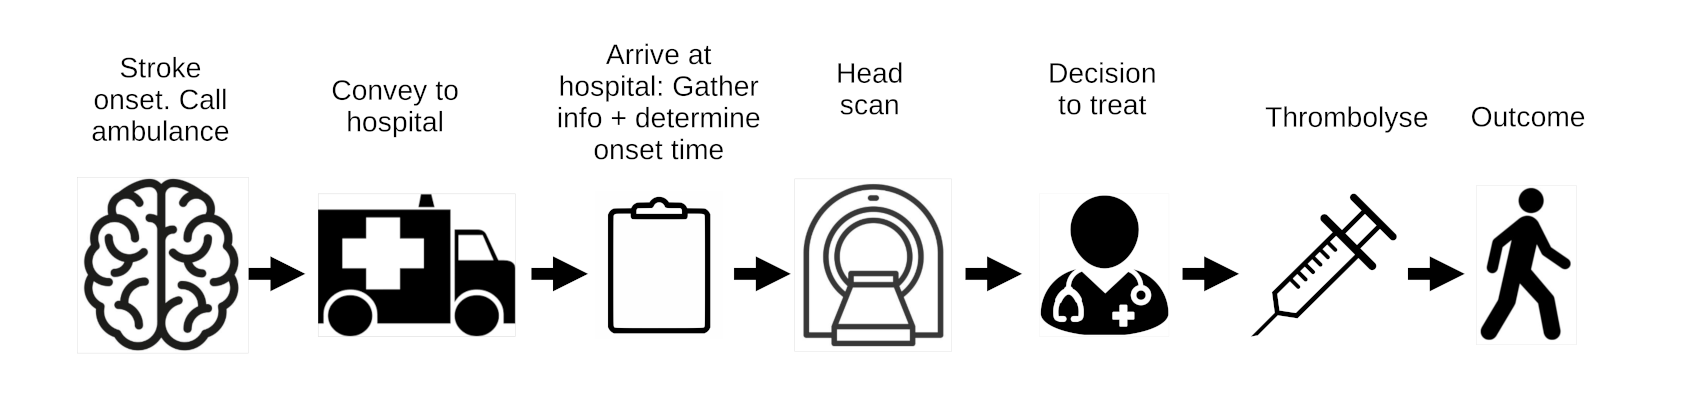
\includegraphics[width=1.0\textwidth]{./images/pathway}
\end{center}

\textbf{To do - all this space looks accidental} 

\end{frame}


%%%%%%%%%%%%%%%%%%%%%%%%%%%%%%%%%%%%%%%%%%%%%%%%%%%%%%%%%%%%%%%

\begin{frame}
\frametitle{A high level view of learning clinical decision-making}

% Don't center this! Leave room for text on the right. 
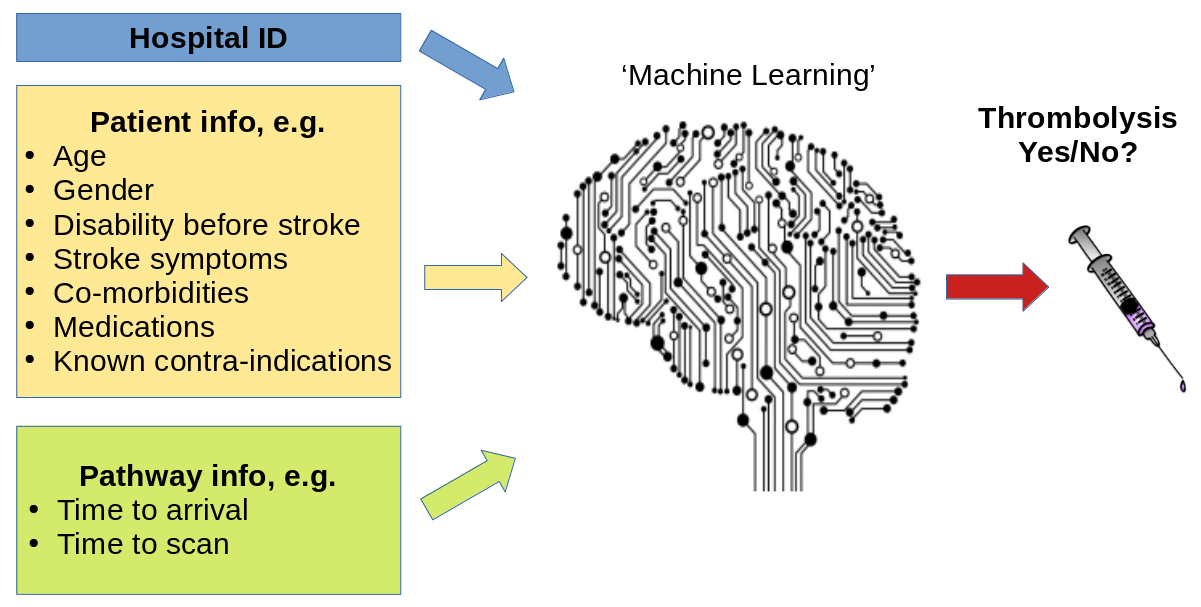
\includegraphics[width=0.8\textwidth]{./images/treatment_decision}


\begin{columns}
    \column{0.35\textwidth}
    % 
    \column{0.65\textwidth}
    \footnotesize
    Machine learning models include logistic regression,
    random forest, XGBoost, and neural networks. 
    
    \vspace{1em}
    
    Here we are using XGBoost models
    \normalsize 
\end{columns}


% Machine learning (and nearly all \emph{artificial intelligence}) is based on the simple principle of recognising similarity to what has been seen before.
% \vspace{3mm}

\vspace{2em}
We accessed 240,000 emergency stroke admissions in England and Wales over three years. %That is a lot of examples to learn from!

\end{frame}




%%%%%%%%%%%%%%%%%%%%%%%%%%%%%%%%%%%%%%%%%%%%%%%%%%%%%%%%%%%%%%%


\begin{frame}
\frametitle{Questions from SAMueL-1}

\footnotesize{We 
% used clinical pathway simulation and machine learning to 
analysed a series of \emph{what if?} questions:}

\begin{itemize}
    \footnotesize
    % \setlength\itemsep{3mm}
    \item What if arrival-to-treatment time was 30 minutes?
    \item What if all hospitals determined stroke onset time as frequently as an \emph{upper quartile} hospital (a hospital ranked 25 out of 100, for determining stroke onset time).
    \item What if decisions to thrombolyse were made according to a majority vote of 30 benchmark hospitals?
\end{itemize}

\footnotesize{For each hospital we use their own patients to ask these questions, to allow for differences in local patient populations.}



% \end{frame}



% %%%%%%%%%%%%%%%%%%%%%%%%%%%%%%%%%%%%%%%%%%%%%%%%%%%%%%%%%%%%%%%

% \begin{frame}
% \frametitle{Results so far from SAMueL-1}
\begin{center}
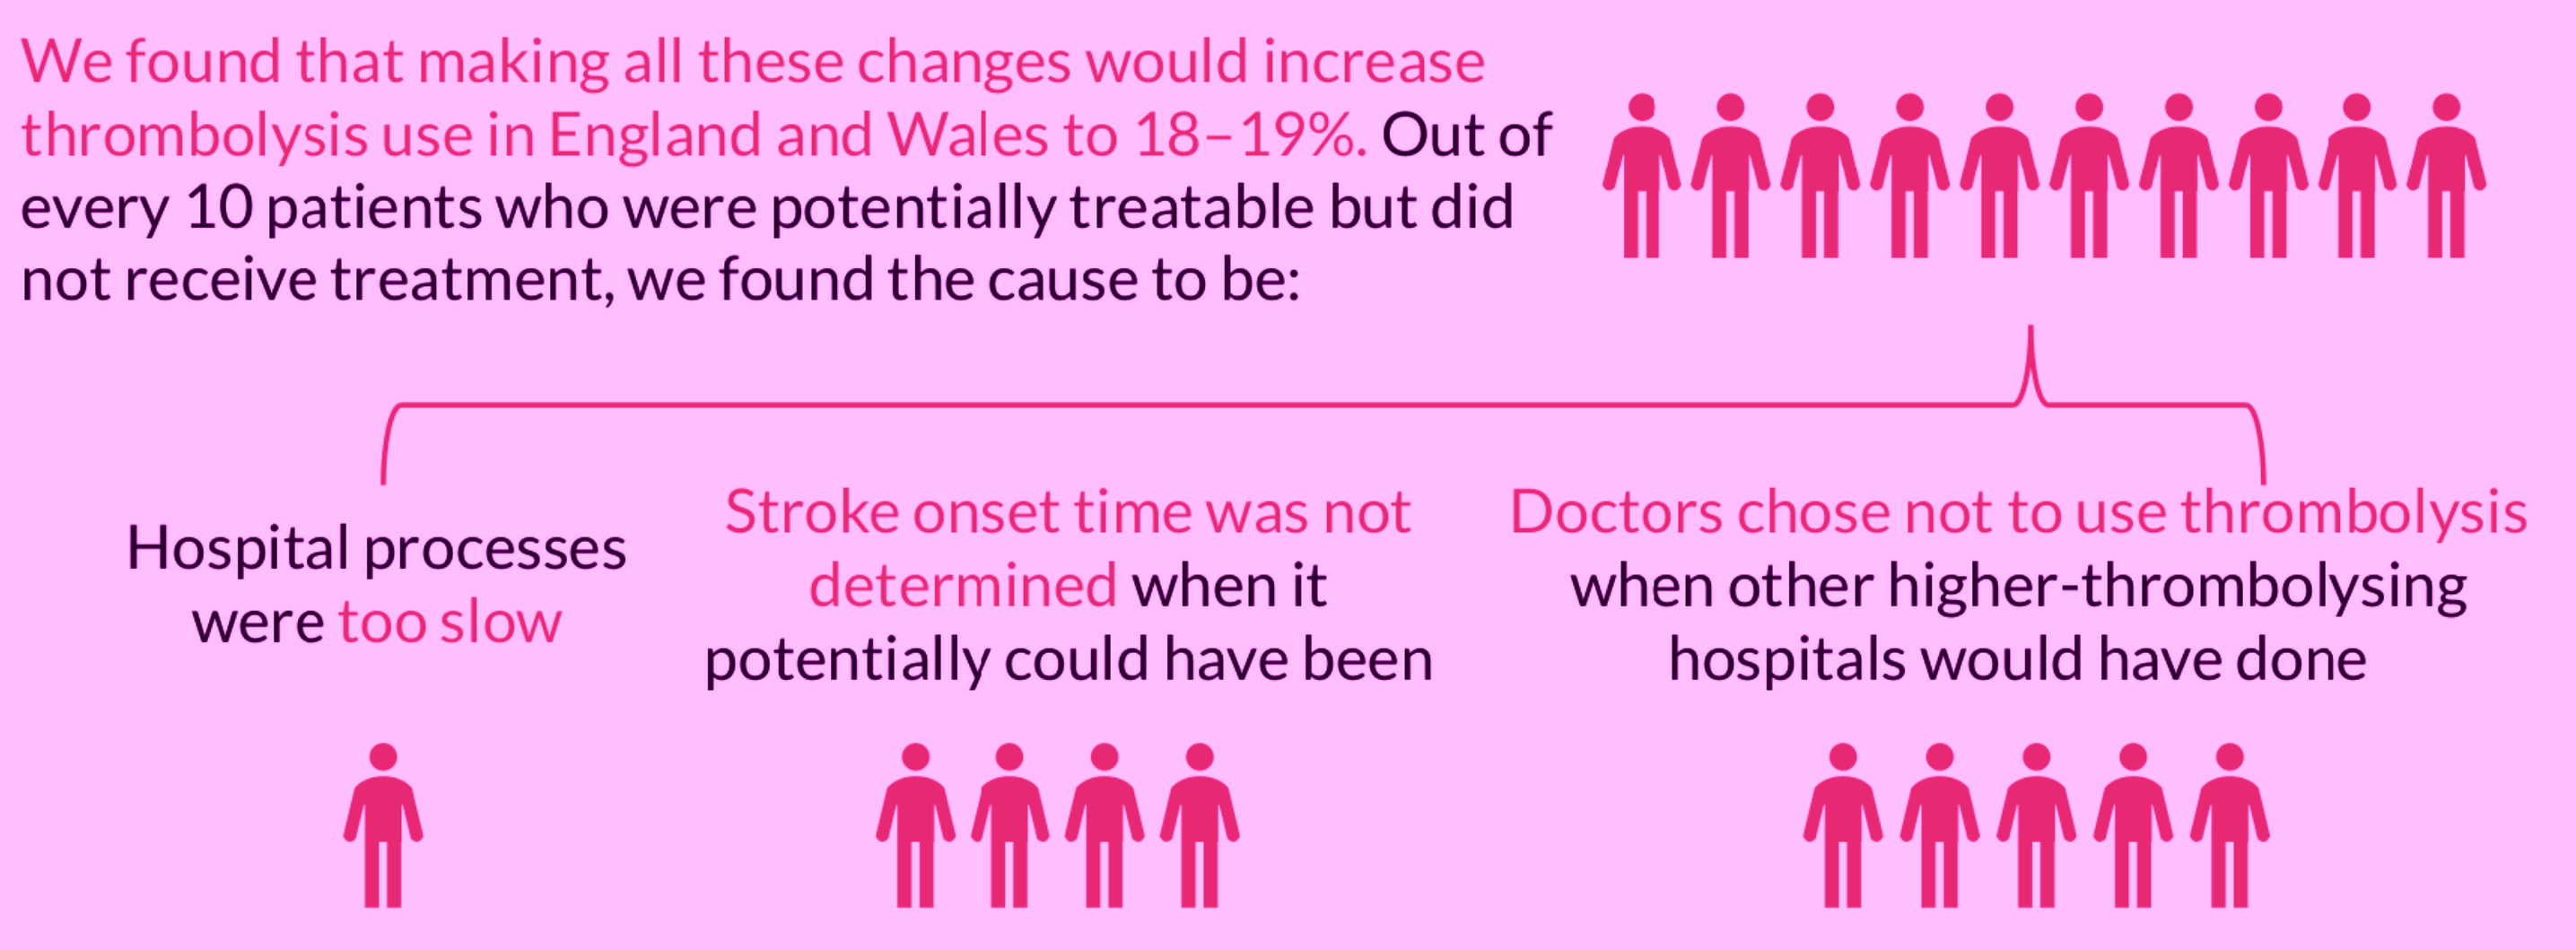
\includegraphics[width=1.0\textwidth]{./images_pink/sam_summary_pt_3}
\end{center}

\end{frame}

%%%%%%%%%%%%%%%%%%%%%%%%%%%%%%%%%%%%%%%%%%%%%%%%%%%%%%%%%%%%%%%

\begin{frame}
\frametitle{What questions are we asking in SAMueL-2?}
\begin{itemize}
    \setlength\itemsep{5mm}
    \item What patients do clinicians agree and disagree on, when considering when they should receive thrombolysis?
    \item How do \emph{organisational factors} (such as use of specialist stroke nurses) affect the thrombolysis pathway and decision-making?
    \item How best can we engage clinicians in our work, and prompt them to reconsider their emergency stroke pathway and/or decision-making?
    
    \begin{itemize}
        \item Communication of general findings.
        \item Web application for individual hospitals.
        \item A 'hospital profile` for each hospital.
    \end{itemize}
\end{itemize}

\end{frame}


%%%%%%%%%%%%%%%%%%%%%%%%%%%%%%%%%%%%%%%%%%%%%%%%%%%%%%%%%%%%%%%
\section{Explainability of neural networks with SHAP}

%%%%%%%%%%%%%%%%%%%%%%%%%%%%%%%%%%%%%%%%%%%%%%%%%%%%%%%%%%%%%%%

% \small Online book: \smallurl{https://samuel-book.github.io/samuel_shap_paper_1/}

% \small View these slides online: \smallurl{https://bit.ly/shap_google_slides}


%%%%%%%%%%%%%%%%%%%%%%%%%%%%%%%%%%%%%%%%%%%%%%%%%%%%%%%%%%%%%%%

\begin{frame}
\frametitle{Simplifying the model with feature selection}

\begin{itemize}
    \tiny 
    \item Our full data set has 85 feature - but which are most important?
    \item A model with fewer features is easier to understand and explain
    \item We build features by selecting them one at a time according to which new feature adds most accuracy
    \item We measure accuracy with ROC-AUC (Receiver Operating Characteristic Curve - Area Under the Curve). But don’t worry about that - it is just a robust accuracy measure.
    \item We find 8 features give us nearly as much accuracy as all features
\end{itemize}

\vspace{0.5em}

\begin{columns}
    \column{0.7\textwidth}
    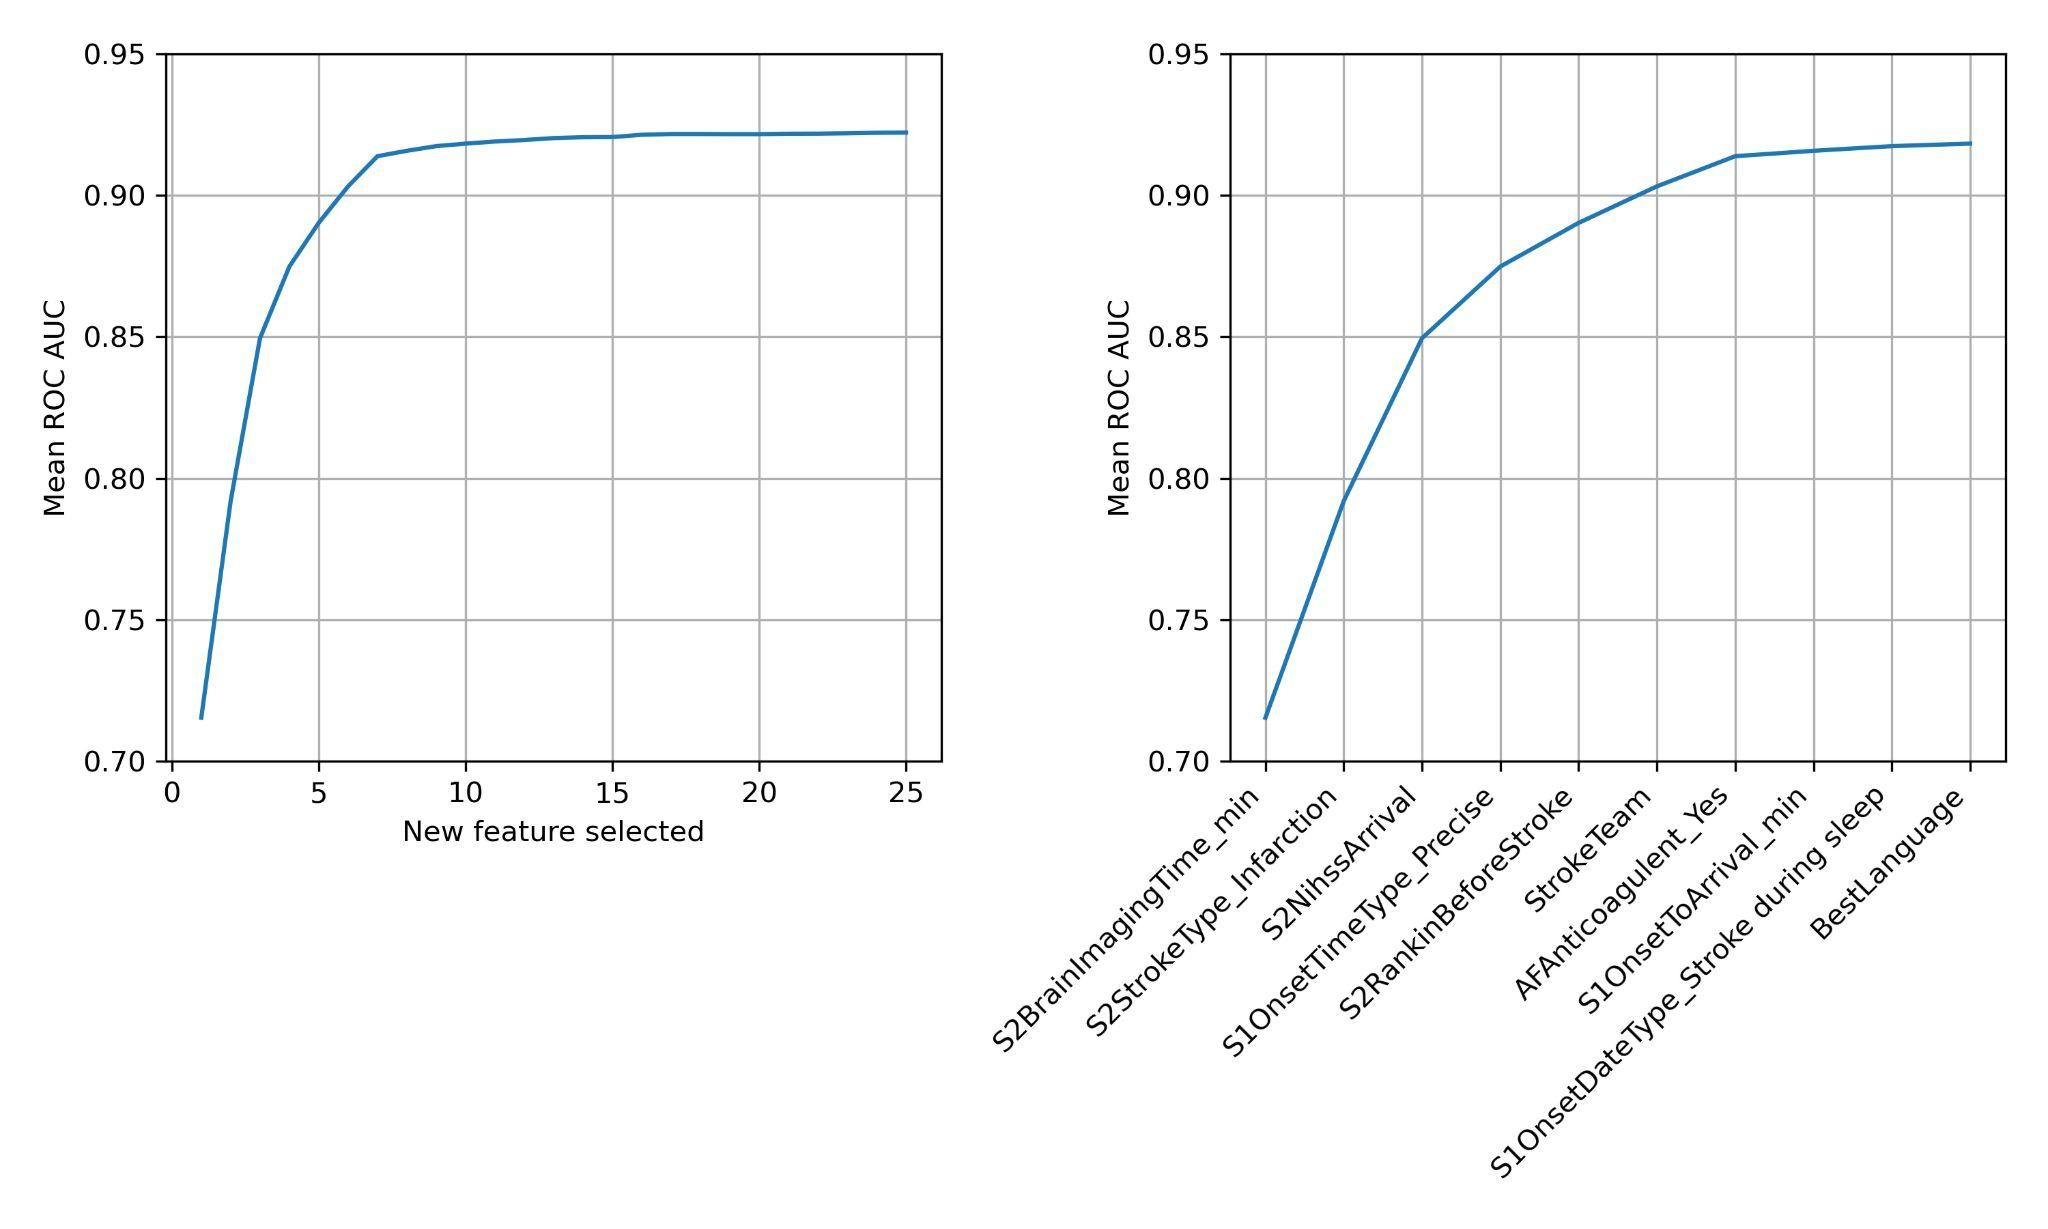
\includegraphics[width=1.0\textwidth]{./images/feature_selection_curves}
    \column{0.25\textwidth}
    \tiny
    Features selected:
    \begin{itemize}
        \tiny
        \item Arrival-to-scan time
        \item Infarction
        \item Stroke severity
        \item Precise onset time
        \item Prior disability level
        \item Stroke team
        \item Use of AF anticoagulants
        \item Onset-to-arrival time
    \end{itemize}
    \normalsize 
\end{columns}

\smallurl{https://samuel-book.github.io/samuel_shap_paper_1/xgb_with_feature_selection/01_xgb_combined_fit_feature_selection.html}

\end{frame}


%%%%%%%%%%%%%%%%%%%%%%%%%%%%%%%%%%%%%%%%%%%%%%%%%%%%%%%%%%%%%%%

\begin{frame}
\frametitle{Model accuracy after selection of 8 features}

\vspace{-1em} 

\begin{center}
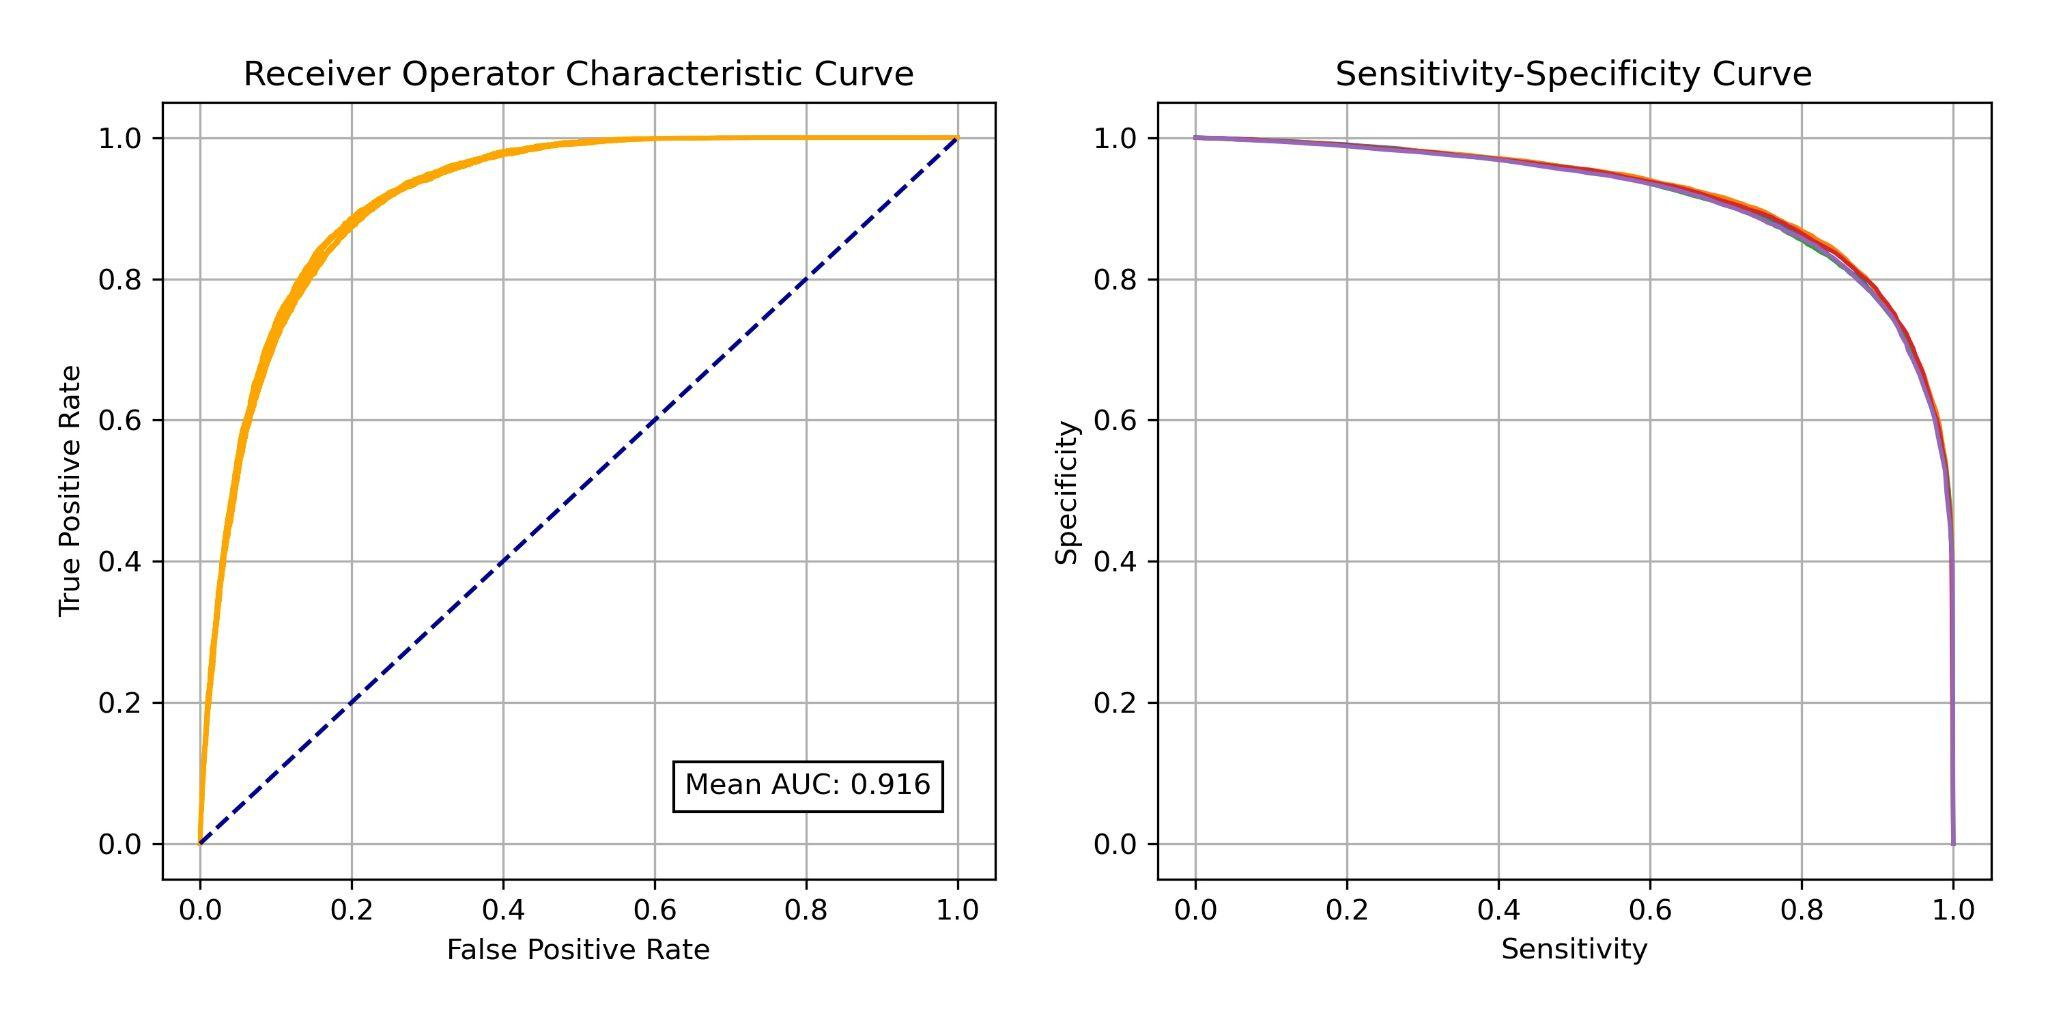
\includegraphics[width=0.8\textwidth]{./images/model_accuracy_with_8_features}
\end{center}

\vspace{-1em}

\begin{itemize}
    \footnotesize 
    \item Accuracy = 85\%
    \item ROC AUC = 0.916
    \item The model can achieve 84\% sensitivity and specificity simultaneously
    \begin{itemize}
        \tiny
        \item Sensitivity: The proportion of patients who receive thrombolysis who are correctly classified
        \item Specificity: The proportion of patients who do not receive thrombolysis who are correctly classified
    \end{itemize} 
\end{itemize}

\smallurl{https://samuel-book.github.io/samuel_shap_paper_1/xgb_with_feature_selection/02_xgb_combined_fit_accuracy_key_features.html}
\end{frame}



%%%%%%%%%%%%%%%%%%%%%%%%%%%%%%%%%%%%%%%%%%%%%%%%%%%%%%%%%%%%%%%

\begin{frame}
\frametitle{Shapley (SHAP) values}

{\footnotesize
SHAP values report how individual patient features affect the model prediction. 
\vspace{0.5em}

SHAP values are usually reported as log odds shift in odds. That is not very intuitive! 
But let’s look at an example of how that feeds into probabilities.
} 

\begin{center} 
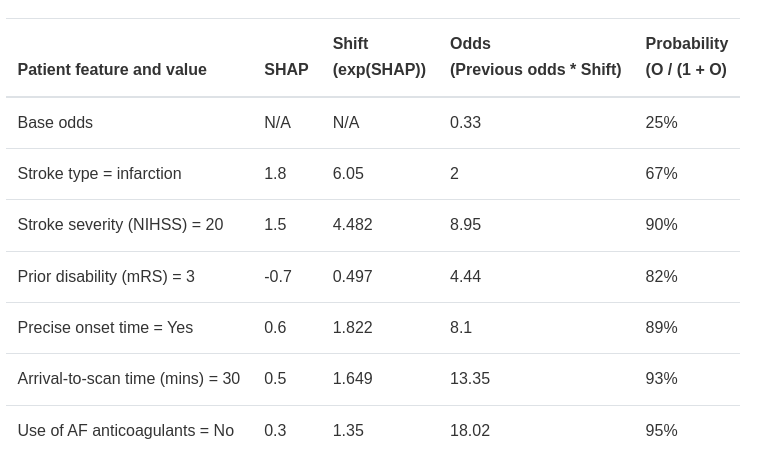
\includegraphics[width=0.7\textwidth]{./images/SHAP_values_table}
\end{center} 

{\tiny For more on odds, probabilities and SHAP see: }
\smallurl{https://samuel-book.github.io/samuel_shap_paper_1/introduction/odds_prob.html}

\end{frame}




%%%%%%%%%%%%%%%%%%%%%%%%%%%%%%%%%%%%%%%%%%%%%%%%%%%%%%%%%%%%%%%

\begin{frame}
\frametitle{How do different SHAP values affect a starting probability of 25\%?}

Let’s build more intuition on the effect of different magnitudes of SHAP.

\begin{center}
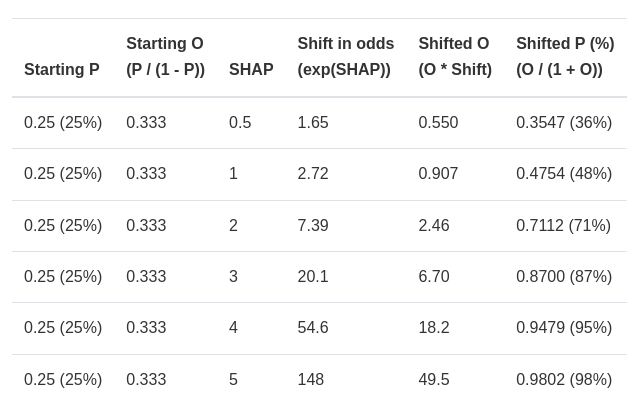
\includegraphics[width=0.7\textwidth]{./images/shap_affect_probability}
\end{center} 

\end{frame}


%%%%%%%%%%%%%%%%%%%%%%%%%%%%%%%%%%%%%%%%%%%%%%%%%%%%%%%%%%%%%%%

\begin{frame}
\frametitle{SHAP output for an individual patient}


SHAP values show the influence of features (even for \emph{`black box'} models).

\begin{center} 
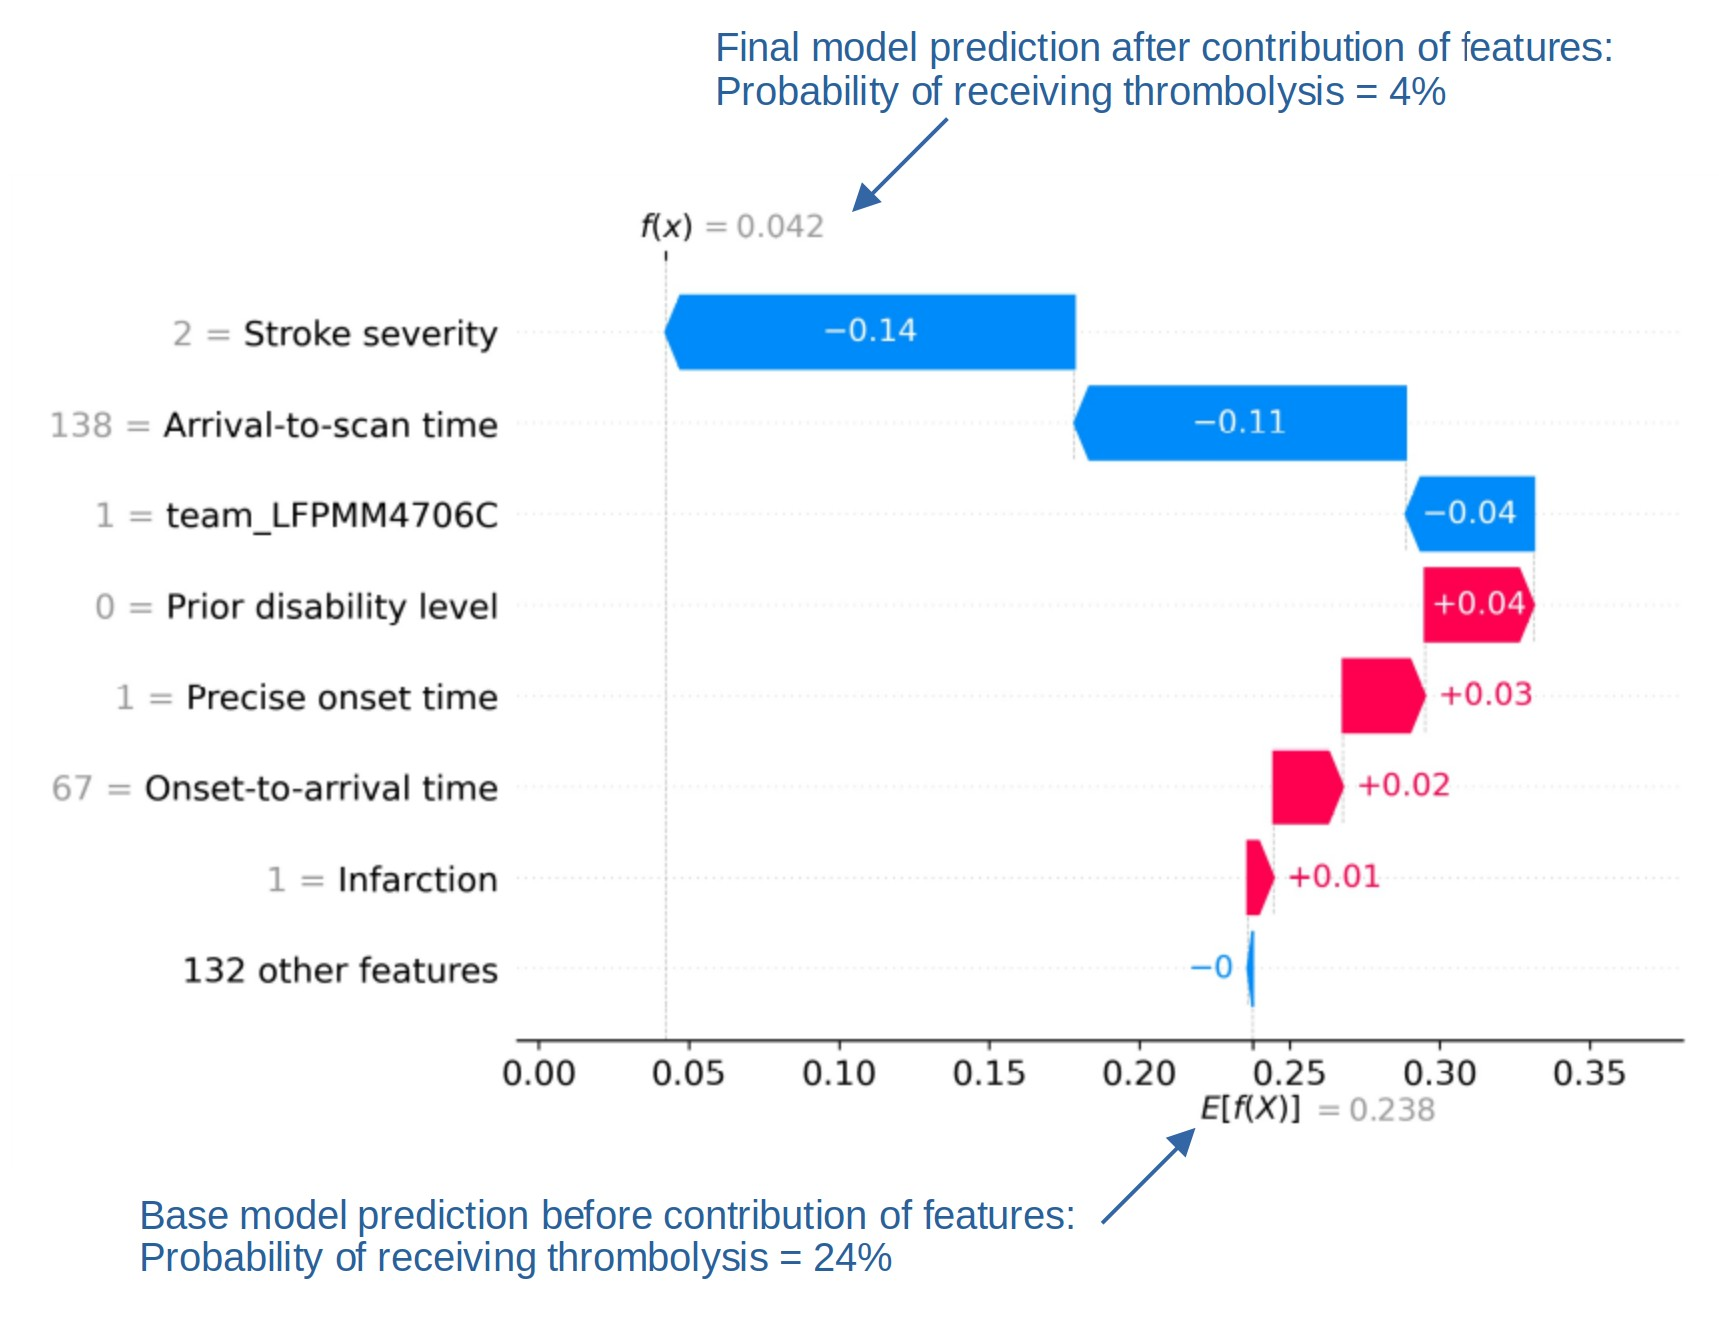
\includegraphics[width=0.8\textwidth]{./images/shap_output_for_individual_patient}
\end{center}

\vspace{-0.8em}
\tiny{Note: SHAP values here are \emph{log odds}. Each step-change in value of \textpm 1 changes the chances of receiving thrombolysis about 3-fold. (Plots are in order of feature importance.)}

\end{frame}



%%%%%%%%%%%%%%%%%%%%%%%%%%%%%%%%%%%%%%%%%%%%%%%%%%%%%%%%%%%%%%%

\begin{frame}
\frametitle{SHAP values for predicting use of thrombolysis across all hospitals}



\vspace{-0.5em}

\begin{center}
    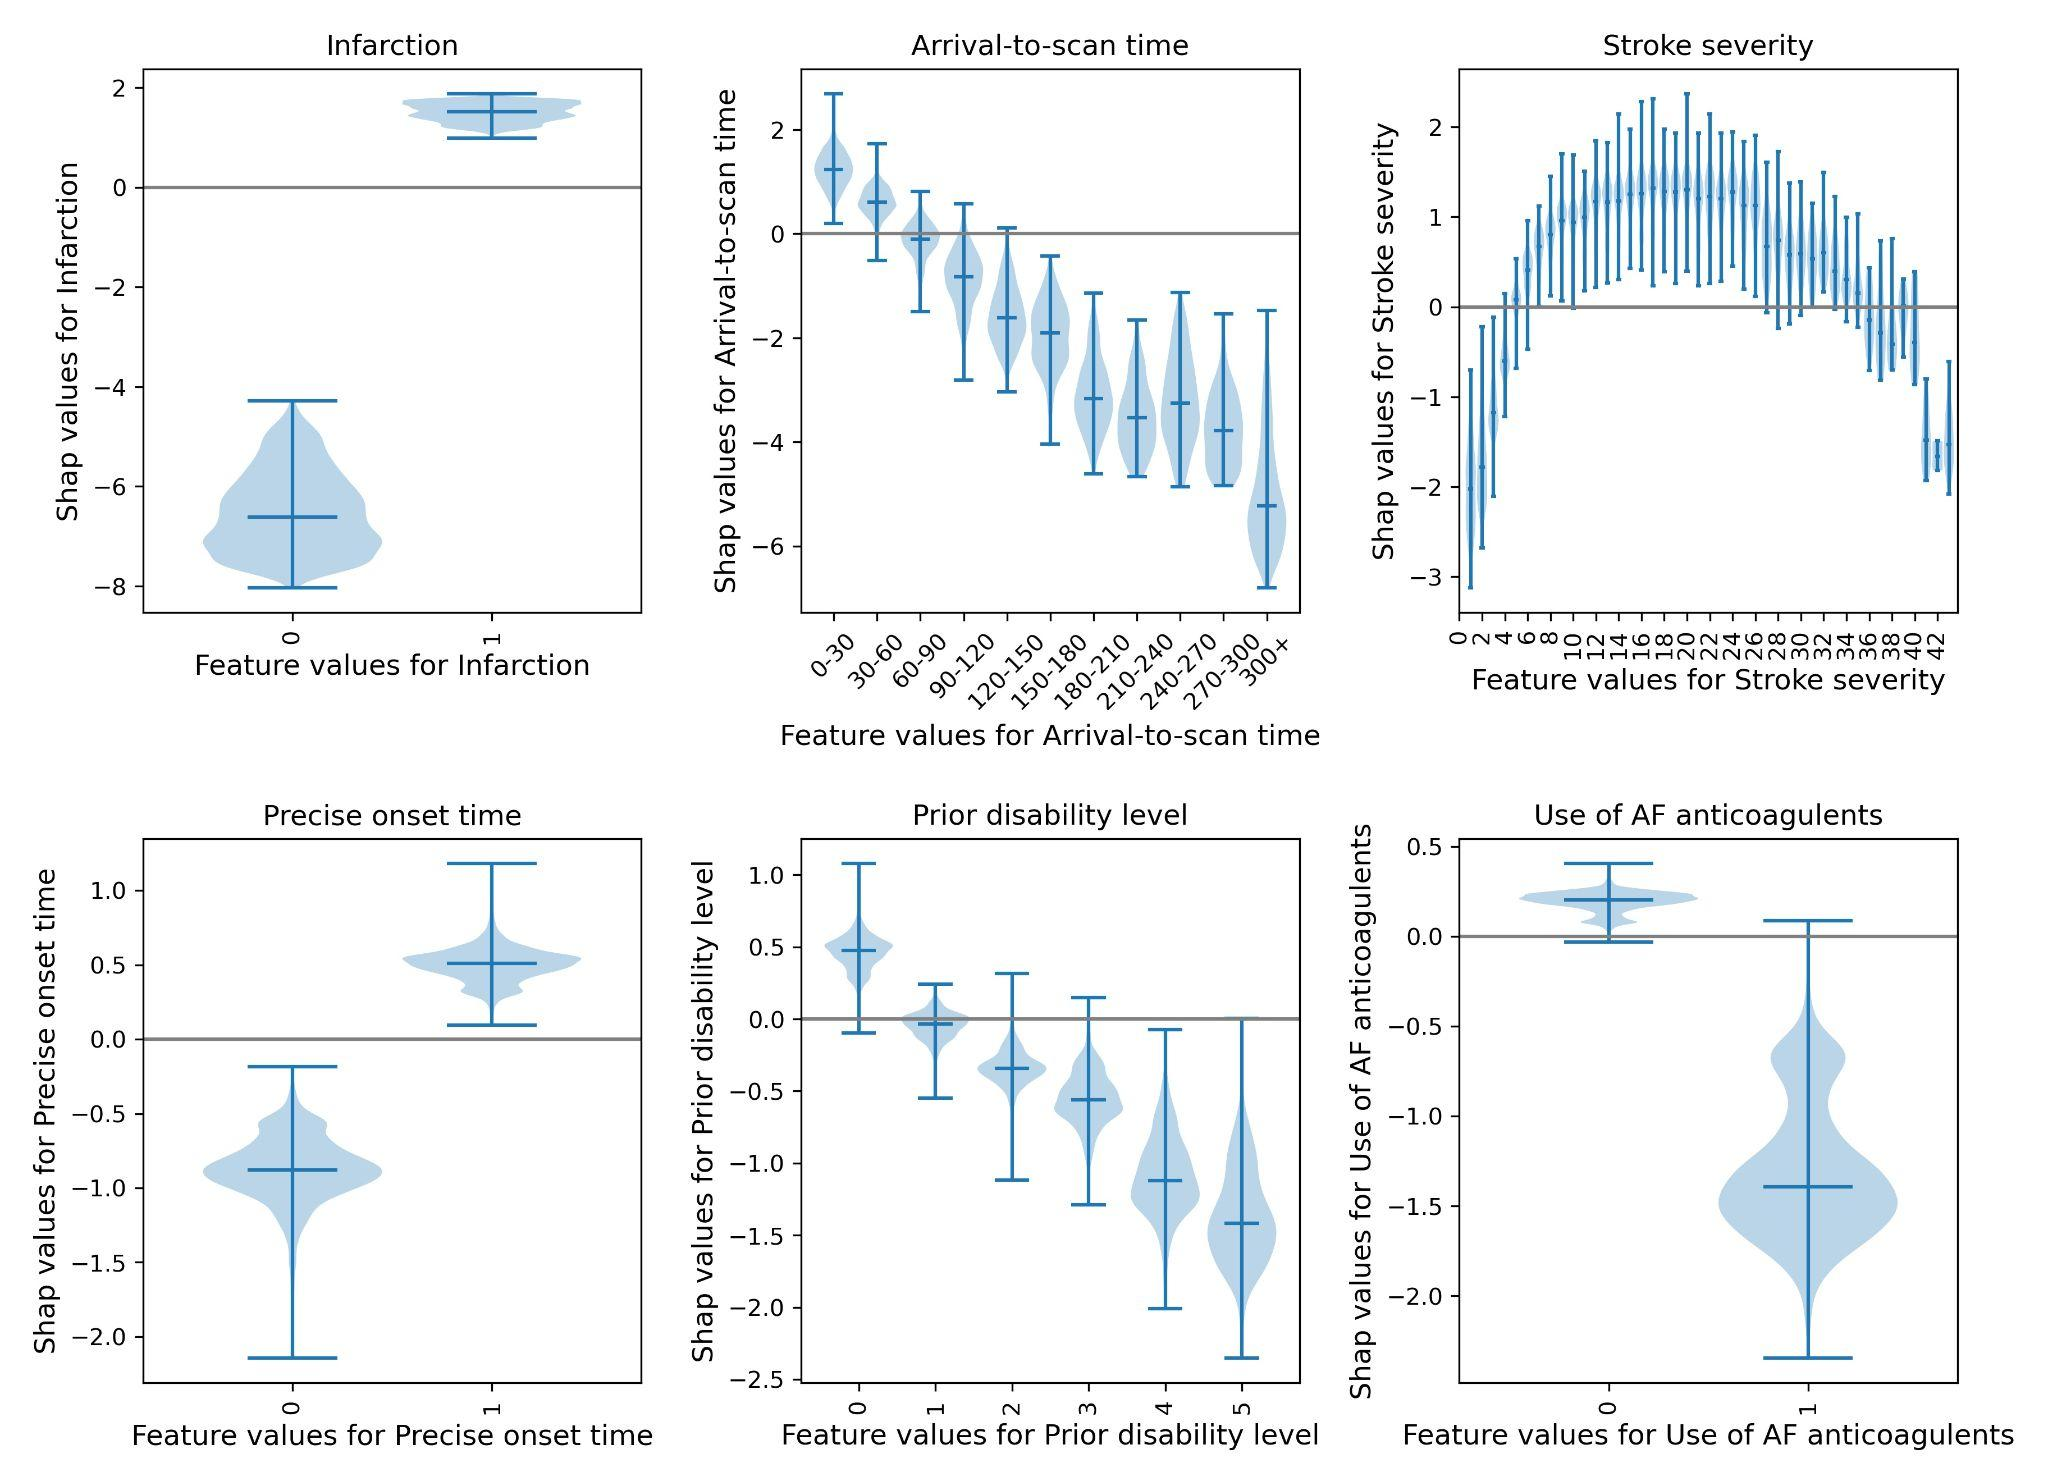
\includegraphics[width=0.75\textwidth]{./images/shap_violins}
\end{center}

\vspace{-1em}

\smallurl{https://samuel-book.github.io/samuel_shap_paper_1/xgb_with_feature_selection/03_xgb_combined_shap_key_features.html}

\end{frame}






%%%%%%%%%%%%%%%%%%%%%%%%%%%%%%%%%%%%%%%%%%%%%%%%%%%%%%%%%%%%%%%

\begin{frame}
\frametitle{10k cohort thrombolysis, and benchmark hospitals}
% \includegraphics[width=1.0\textwidth]{./images/}

\begin{itemize}
  \item Separate out 10k patients 
  \item Train model on remaining data (78,792 patients)
  \item Pass 10k cohort through model, changing hospital coding each time to mimic same patients going to each of 132 hospitals
  \begin{itemize} 
    \item All other patient and pathway data the same each time
  \end{itemize} 
  \item Model then predicts the thrombolysis rate across hospitals if they all saw the same patients
  \item Top 30 thrombolysing hospitals are taken as ‘benchmark’
hospital
  \begin{itemize} 
    \item A ‘benchmark decision’ on any patient may be made by taking the majority vote of the benchmark hospitals
  \end{itemize} 
\end{itemize}


{\tiny
Note: Here we are looking at the predicted use of thrombolysis in patients who arrive within 4 hours of
known stroke onset (this is about 40\% of all emergency stroke admissions).}


\end{frame}


%%%%%%%%%%%%%%%%%%%%%%%%%%%%%%%%%%%%%%%%%%%%%%%%%%%%%%%%%%%%%%%

\begin{frame}
\frametitle{Average SHAP values for each hospital}

Average SHAP values for each hospital range from -1.3 to +1.3.

\begin{columns}
    \column{0.57\textwidth}
    \begin{center} 
    \includegraphics[width=\textwidth]{./images/shap_average_per_hospital_annotated}
    \end{center}


    \column{0.43\textwidth}
    \vspace{0.5em}
    \begin{center} 
    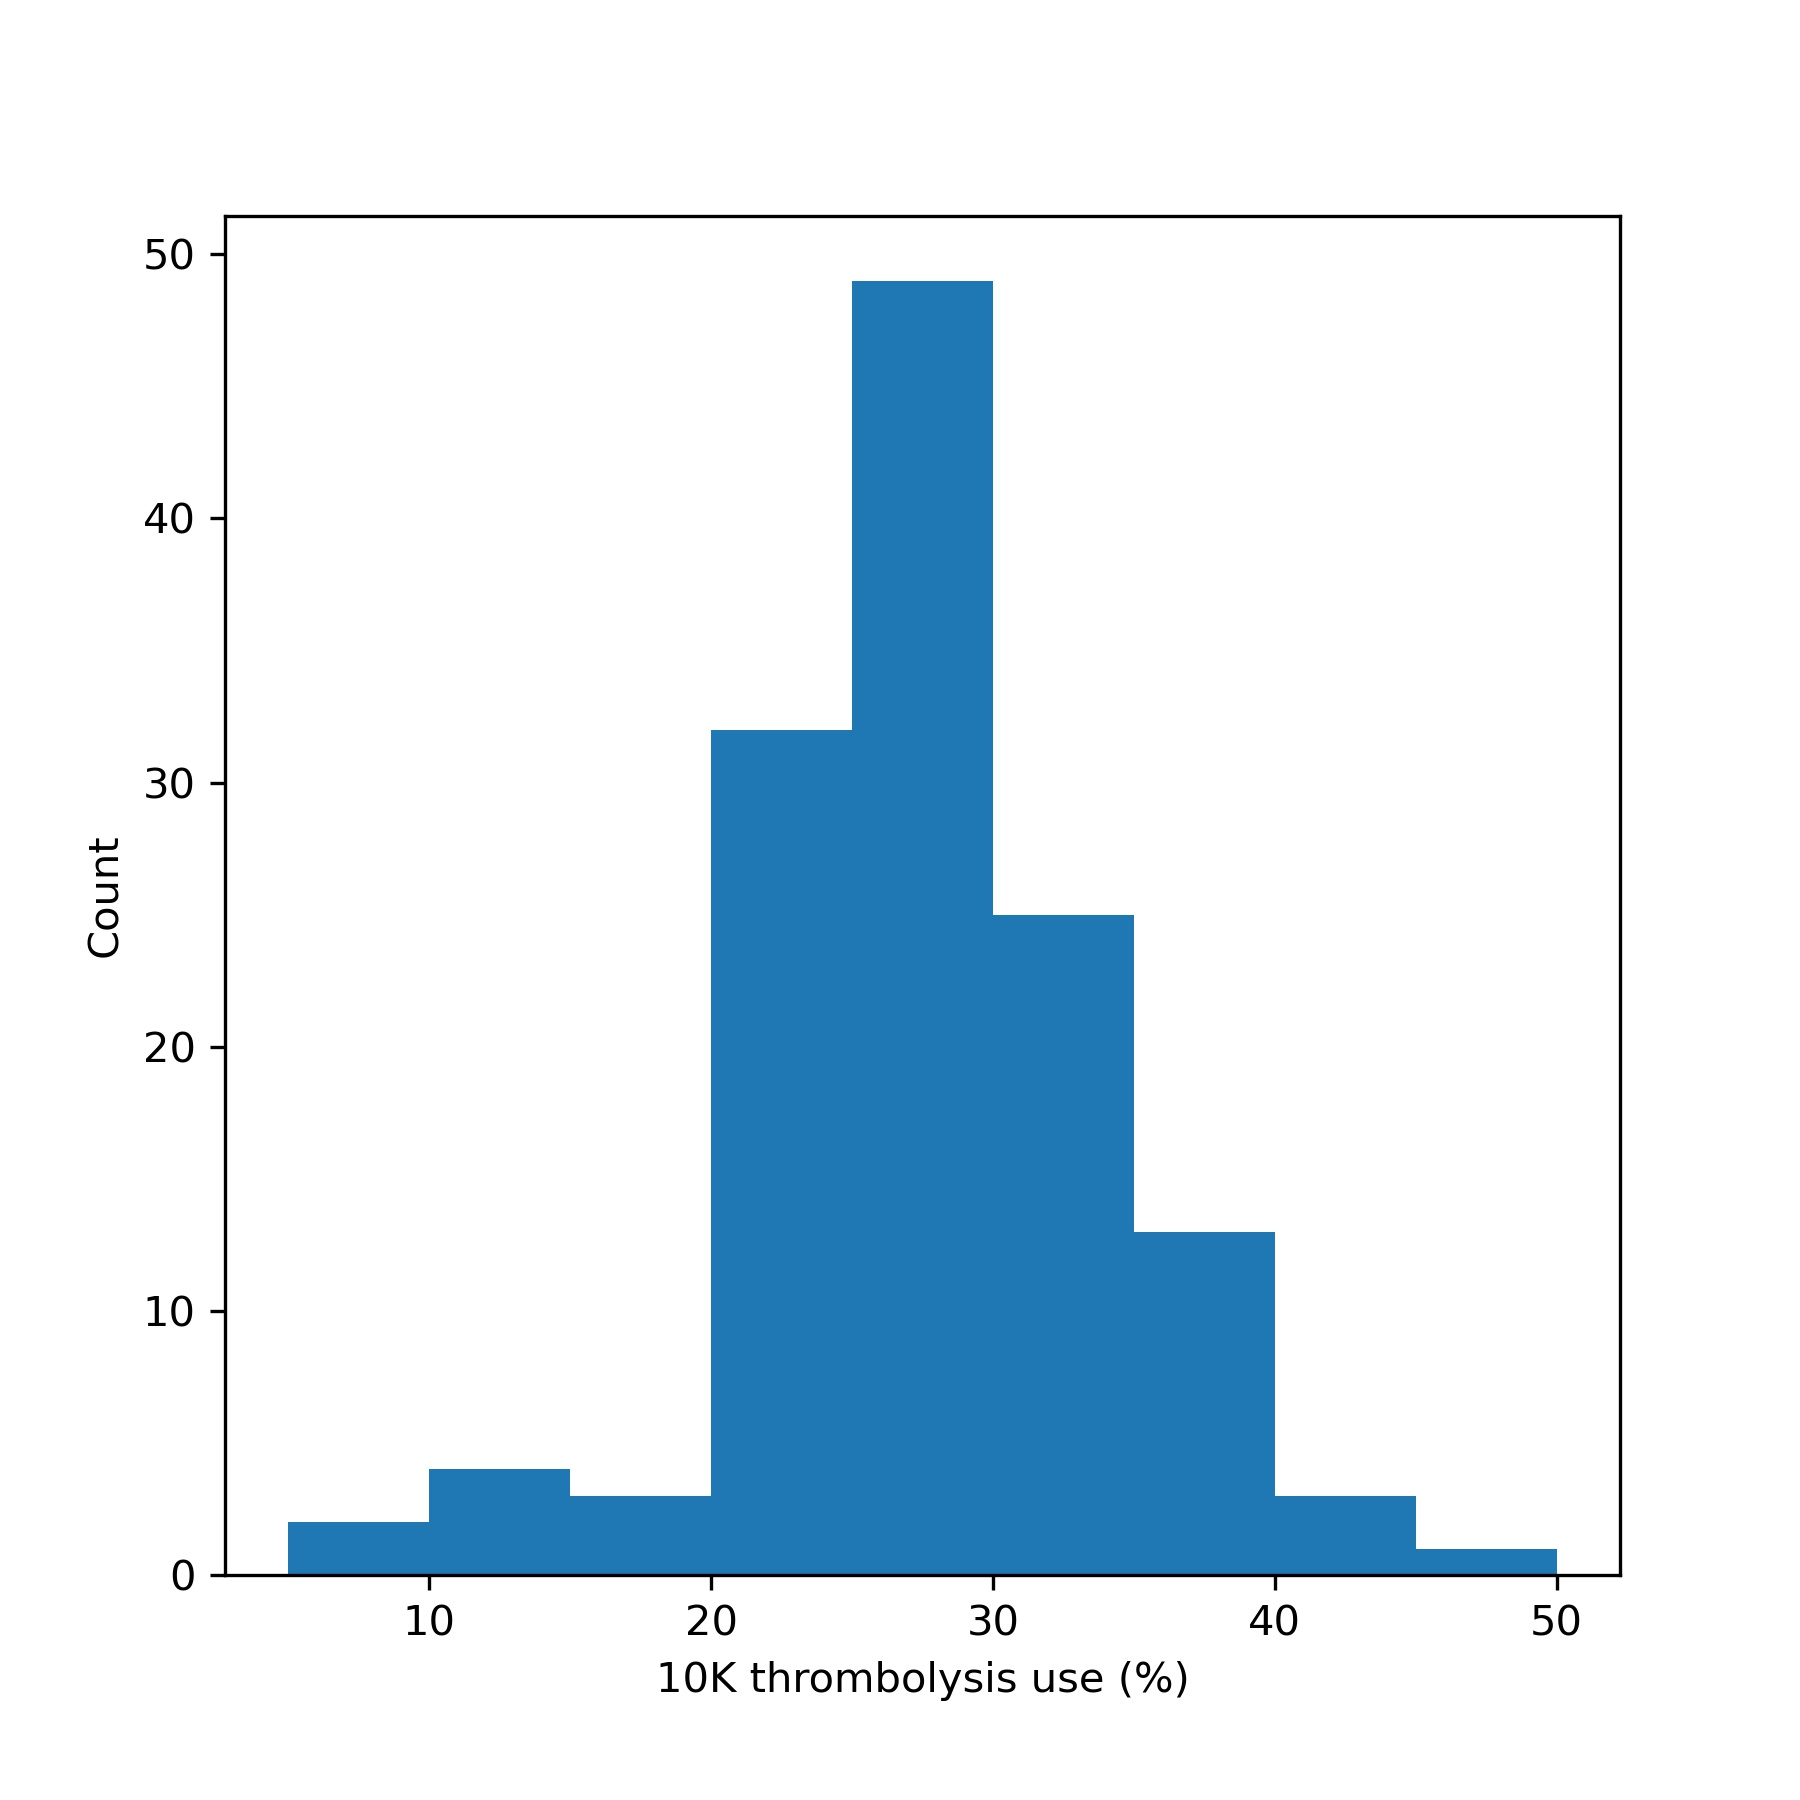
\includegraphics[width=\textwidth, trim={0em 0em 0em 4em}, clip]{./images/predicted_thrombolysis_use}
    \end{center} 

\end{columns} 



\smallurl{https://samuel-book.github.io/samuel_shap_paper_1/xgb_with_feature_selection/03_xgb_combined_shap_key_features.html}

\smallurl{https://samuel-book.github.io/samuel_shap_paper_1/xgb_with_feature_selection/04_compare_10k_cohort_key_features.html}


\end{frame}


%%%%%%%%%%%%%%%%%%%%%%%%%%%%%%%%%%%%%%%%%%%%%%%%%%%%%%%%%%%%%%%

\begin{frame}
\frametitle{How does the predicted 10k thrombolysis use compare with the SHAP values learned for each hospital?}

\begin{columns}
    \column{0.8\textwidth}
    \begin{center} 
    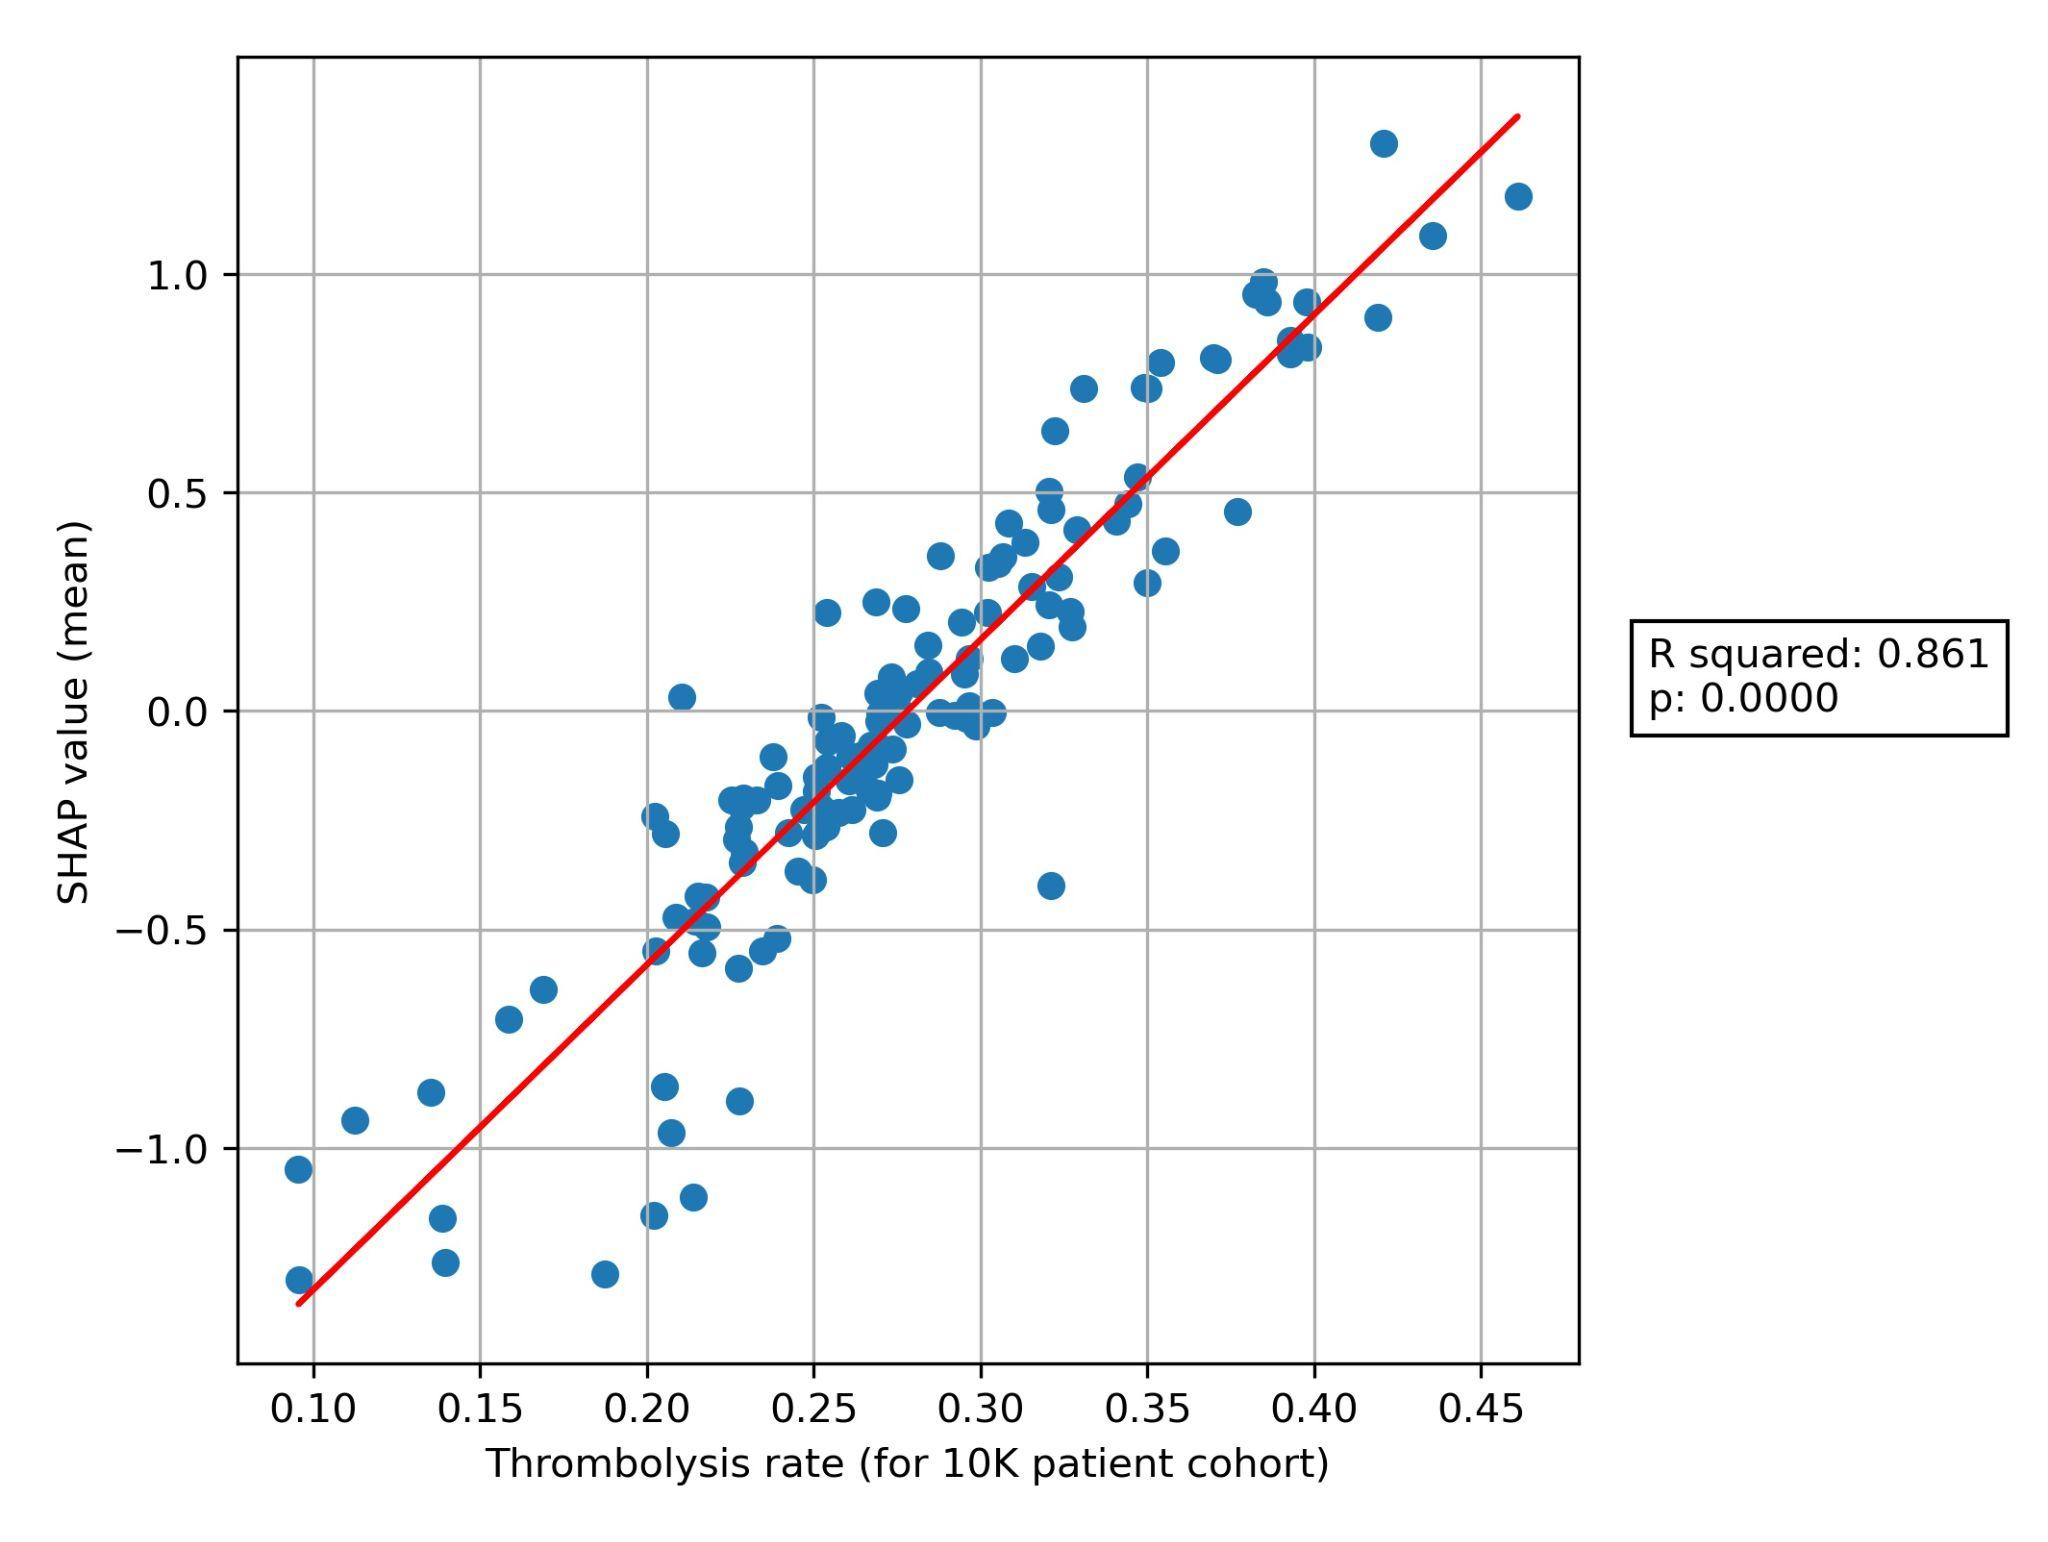
\includegraphics[width=0.98\textwidth]{./images/rsquared_shap_predicted_thrombolysis}
    \end{center} 
    
    \column{0.2\textwidth}
    
    {\footnotesize
    86\% of the variance in predicted
    10k thrombolysis use can be
    explained by the learned hospital
    SHAP.}
\end{columns}


\end{frame}


%%%%%%%%%%%%%%%%%%%%%%%%%%%%%%%%%%%%%%%%%%%%%%%%%%%%%%%%%%%%%%%

\begin{frame}
\frametitle{Learning differences in decision-making between hospitals with low and high propensity to thrombolysis}

\vspace{-0.5em}

\begin{itemize}
  \footnotesize
  \item Low thrombolysing hospitals = lowest predicted 10k thrombolysis use
  \item  High thrombolysing hospitals = highest predicted 10k thrombolysis use
\end{itemize} 

\vspace{1.5em}

\textcolor{SkyBlue}{\textbf{Motivation:} ``What patients do low thrombolysing hospitals not thrombolyse, when high thrombolysing hospitals would?''} 

\vspace{1.5em}

Model:
\begin{itemize}
  \footnotesize
  \item Get data for all patients attending low thrombolysing hospitals
  \item Find those patients who would be given thrombolysis by a majority of the high thrombolysing hospitals
  \item Train a model to predict which of those patients would be treated differently at the lower low thrombolysing hospitals (i.e. would not receive thrombolysis)
\end{itemize}

\end{frame}


%%%%%%%%%%%%%%%%%%%%%%%%%%%%%%%%%%%%%%%%%%%%%%%%%%%%%%%%%%%%%%%

\begin{frame}
\frametitle{Accuracy of model to predict differences in clinical decision-making}

\vspace{-0.5em}
\begin{center} 
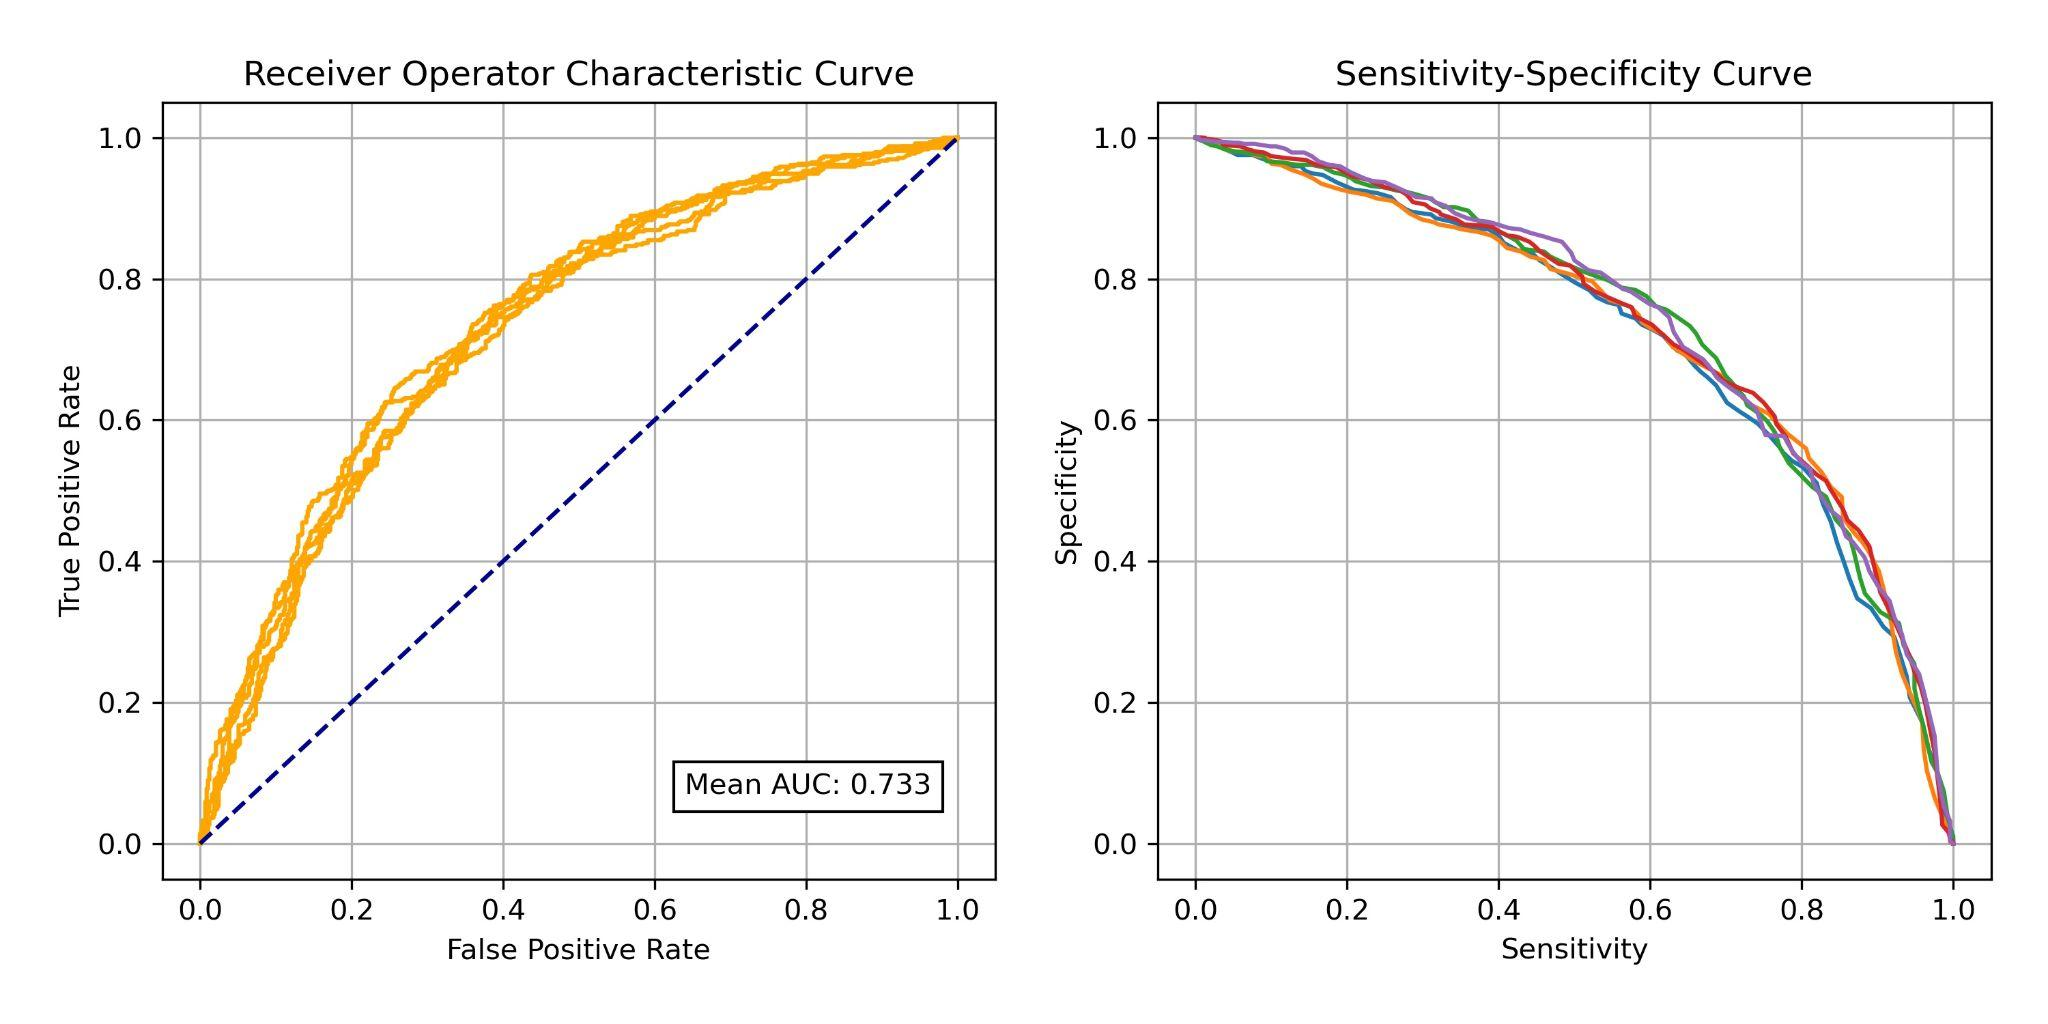
\includegraphics[width=0.8\textwidth]{./images/accuracy_of_model_to_predict_differences_in_clinical_decision-making}
\end{center} 

\vspace{-1em}
\begin{itemize}
  \tiny
  \item Accuracy = 67\%
  \item ROC AUC = 0.733
  \item The model can achieve 67\% sensitivity and specificity simultaneously
  \begin{itemize}
    \tiny
    \item Sensitivity: The proportion of patients who receive thrombolysis who are correctly classified
    \item Specificity: The proportion of patients who do not receive thrombolysis who are correctly classified
  \end{itemize} 
\end{itemize} 

% \vspace{1.5em}

\smallurl{https://samuel-book.github.io/samuel_shap_paper_1/xgb_with_feature_selection/06_predict_differences_between_local_and_benchmark_key_features.html}

\end{frame}


%%%%%%%%%%%%%%%%%%%%%%%%%%%%%%%%%%%%%%%%%%%%%%%%%%%%%%%%%%%%%%%

\begin{frame}
\frametitle{SHAP values for predicting when a low thrombolysis use hospital would \textbf{not} use thrombolysis when a high thrombolysis use hospital would}


\tiny{Here, a high SHAP shows when a low-thrombolysing unit will reject use of thrombolysis when a higher thrombolysing hospital would use thrombolysis. (Plots are in order of feature importance.)}

\vspace{-0.5em}
\begin{center} 
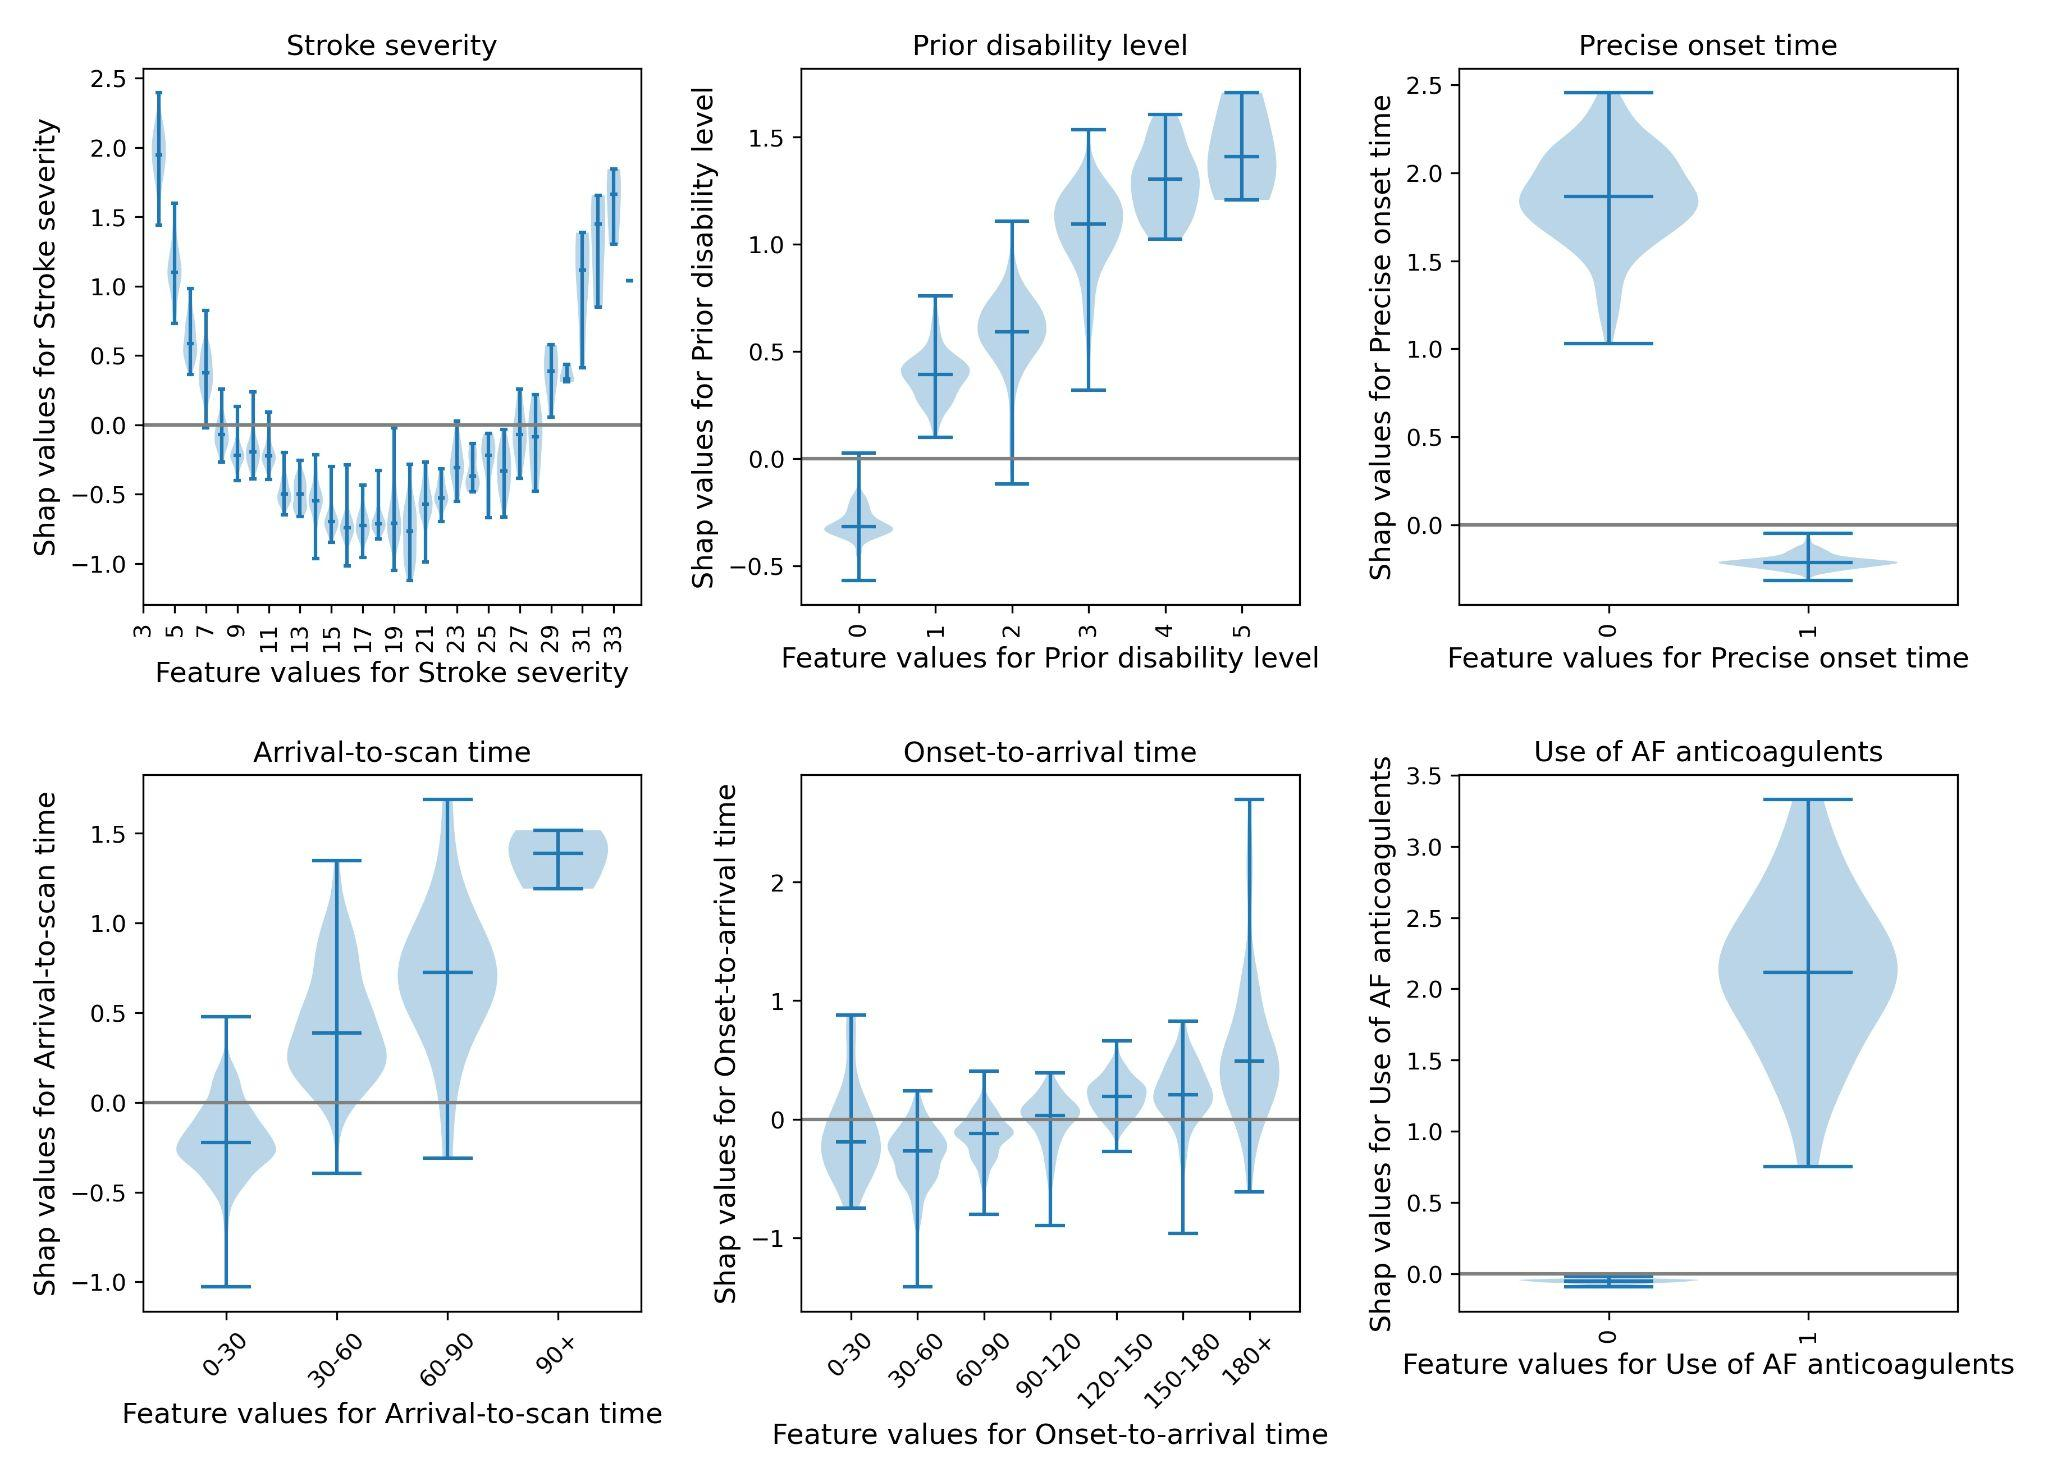
\includegraphics[width=0.75\textwidth, trim=0 0 0 2.5em, clip]{./images/shap_not_use_thrombolysis}
\end{center} 

\vspace{-1.3em}
\smallurl{https://samuel-book.github.io/samuel_shap_paper_1/xgb_with_feature_selection/08_xgb_combined_fit_shap_high_vs_low_thrombolysing_units.html}

\end{frame}

%%%%%%%%%%%%%%%%%%%%%%%%%%%%%%%%%%%%%%%%%%%%%%%%%%%%%%%%%%%%%%%

\begin{frame}
\frametitle{Who are the low thrombolysing hospitals not giving thrombolysis to?}

We find that low thrombolysing hospitals are less likely to give thrombolysis to patients with:

\begin{itemize}
  \item Low or very high stroke severity
  \item An estimated (not precise) stroke onset time
  \item Prior disability
  \item A longer arrival-to-scan time
  \item Use of of AF anticoagulants
  \item A longer onset-to-arrival time
\end{itemize}

\vspace{2em}

These are the same patterns as we see in general thrombolysis decision-making,
but low thrombolysing hospitals appear more sensitive to these features.

\end{frame}

%%%%%%%%%%%%%%%%%%%%%%%%%%%%%%%%%%%%%%%%%%%%%%%%%%%%%%%%%%%%%%%

\begin{frame}
\frametitle{SHAP Summary}

\begin{columns}
    \column{0.5\textwidth}
    \begin{itemize}
      \footnotesize 
      \item Thrombolysis rates vary considerably (5--25\%)
      \item An XGBoost model with 8 features has 85\% accuracy at predicting use of thrombolysis
      \item Shapley (or SHAP) values show how much each feature influences the model prediction
      \item The probability of receiving thrombolysis is increased with:
      \begin{itemize}
        \tiny 
        \item Ischaemic stroke
        \item Short arrival to scan time
        \item Stroke severity 6-35
        \item Precisely known onset time
        \item Low prior disability
        \item No use of anticoagulants for AF
        \item Short onset-to-arrival times
        \item Attending hospitals with high propensity to use thrombolysis
      \end{itemize}
    \end{itemize}

    \column{0.5\textwidth} 
    \begin{itemize}
      \footnotesize 
      \item Predicted thrombolysis use in a 10k patient cohort set correlates very well with hospital SHAP values
      \item Applying thrombolysis benchmark decisions would increase thrombolysis use 22\% overall, and 67\% in the 30 hospitals with the lowest propensity to use thrombolysis.
      \item We find that low thrombolysing hospitals are less likely to give thrombolysis to patients with:
      \begin{itemize}
        \tiny 
        \item Low or very high stroke severity
        \item An estimated (not precise) stroke onset time
        \item Prior disability
        \item A longer arrival-to-scan time
        \item A longer onset-to-arrival time
        \item Use of of AF anticoagulants
      \end{itemize}
    \end{itemize}
\end{columns}

\end{frame}


%%%%%%%%%%%%%%%%%%%%%%%%%%%%%%%%%%%%%%%%%%%%%%%%%%%%%%%%%%%%%%%
\section{Outcome modelling}


%%%%%%%%%%%%%%%%%%%%%%%%%%%%%%%%%%%%%%%%%%%%%%%%%%%%%%%%%%%%%%%

\begin{frame}
\frametitle{How do we define outcomes?}

\footnotesize{Modified Rankin Scale (mRS) is a measure of disability or dependence for people with stroke.
Because mRS bands are not linear, we also use utility as a measure of quality of life.}

\begin{center} 
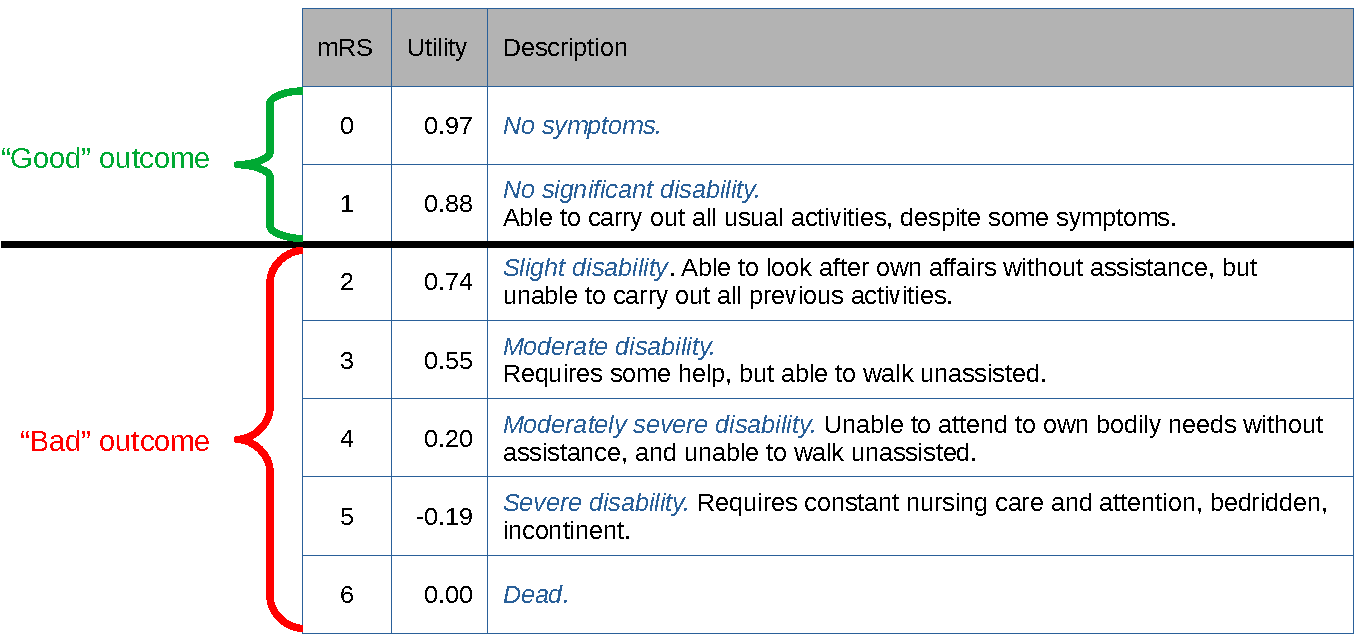
\includegraphics[width=1.0\textwidth]{./images/mRS_table}
\end{center} 

% Utilities are from Wang et al. 2020
%    Wang X, Moullaali TJ, Li Q, Berge E, Robinson TG, Lindley R, et al. 
%    Utility-Weighted Modified Rankin Scale Scores for the Assessment of Stroke
%    Outcome. Stroke. 2020 Aug 1;51(8):2411-7. 

\footnotesize{One of our aims is to calculate changes using all of the mRS bands, so the results are more finely-grained than the previous "good" or "bad" outcome options.}

\end{frame}


%%%%%%%%%%%%%%%%%%%%%%%%%%%%%%%%%%%%%%%%%%%%%%%%%%%%%%%%%%%%%%%

\begin{frame}
\frametitle{Lots of data sources...!}


\begin{center} 
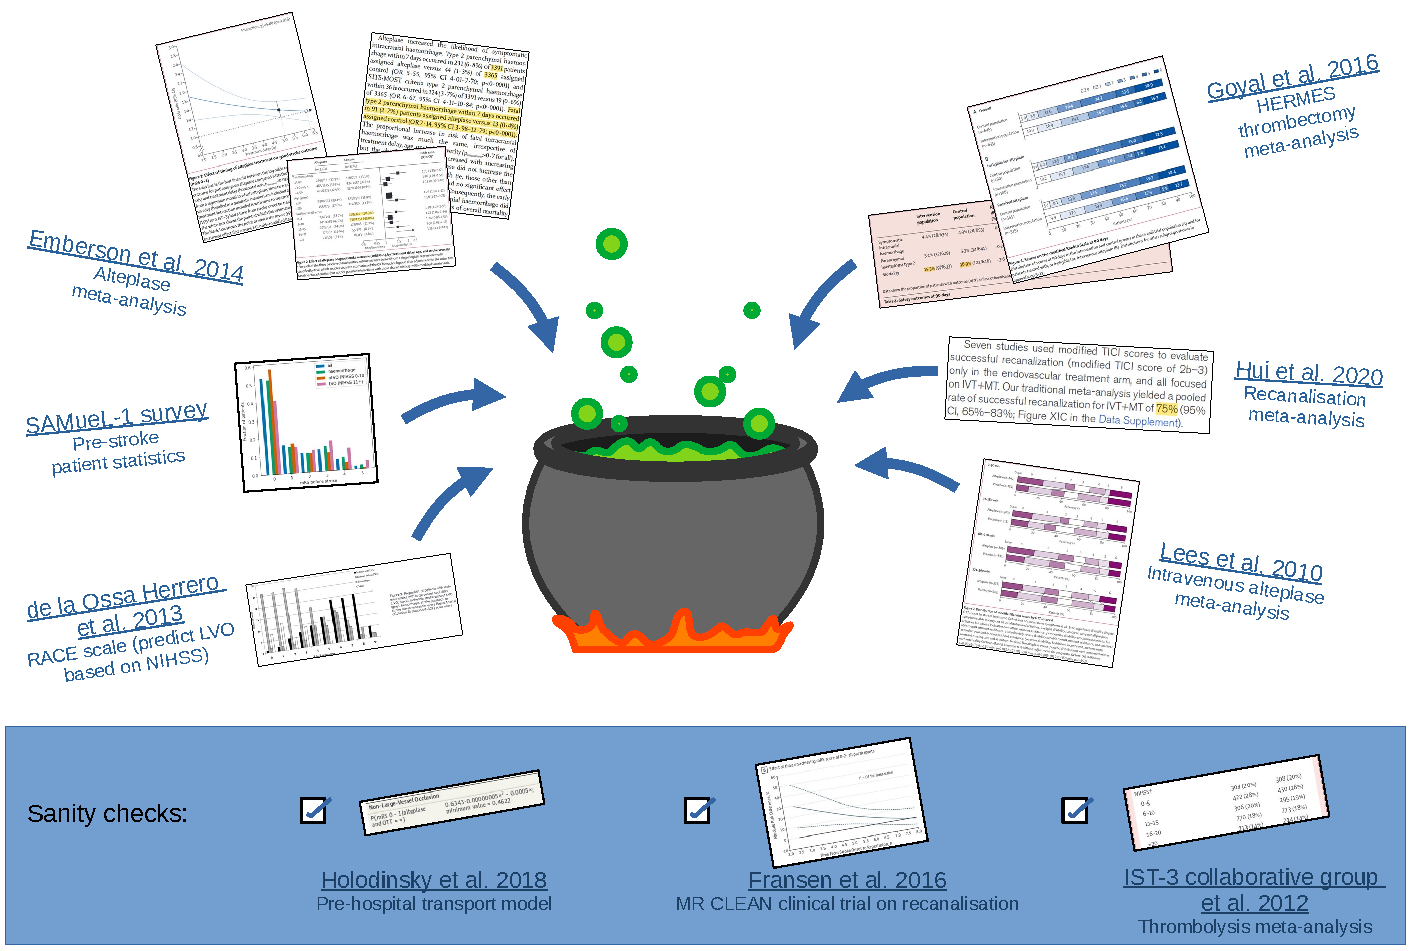
\includegraphics[width=0.95\textwidth]{./images/data_cauldron}
\end{center} 

\vspace{-1em}
\smallurl{https://github.com/samuel-book/stroke_outcome/blob/main/mRS_datasets_full.ipynb}

\vspace{-0.5em}
\smallurl{https://github.com/samuel-book/stroke_outcome/blob/main/bonus_notebooks/data_sources_cheatsheet.ipynb}

\end{frame}


%%%%%%%%%%%%%%%%%%%%%%%%%%%%%%%%%%%%%%%%%%%%%%%%%%%%%%%%%%%%%%%

\begin{frame}
\frametitle{The result: mRS probability distributions}


\begin{center} 
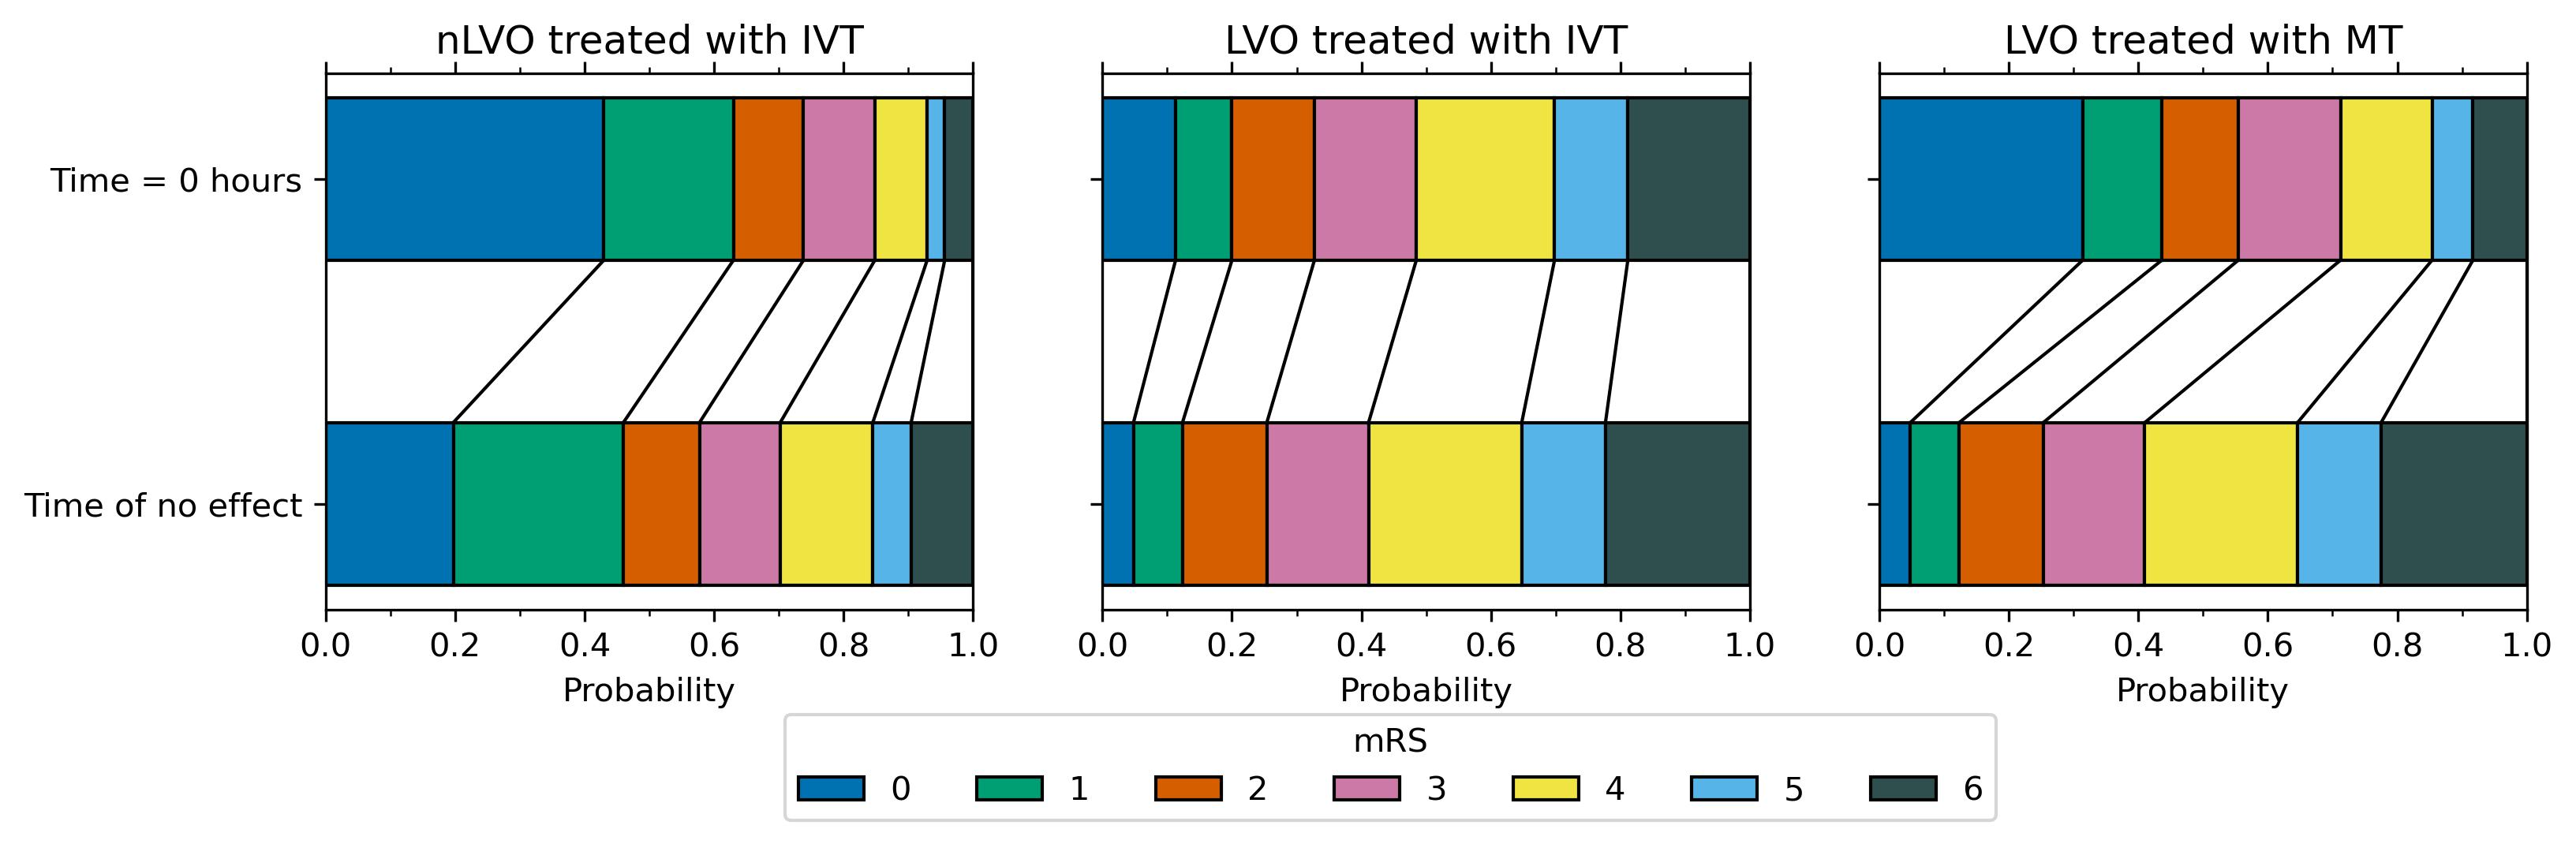
\includegraphics[width=\textwidth]{./images/dist_bars}
\end{center} 


We also create probability distributions for the pre-stroke population and the population that receives no treatment. 

\vspace{0.5em}
    
\begin{columns}

    \column{0.5\textwidth} 
    \begin{description}
        \tiny
        \item[IVT] Intravenous thrombolysis
        \item[MT] Mechanical thrombectomy
        \item[LVO] Large-vessel occlusion
        \item[nLVO] Non-large-vessel occlusion
        % \item[mRS] Modified Rankin scale (disability level where 0=no symptoms and 6=dead)
    \end{description}
    
    % \column{0.\textwidth} 
    % 
    
    \column{0.5\textwidth}
    % Acronyms:
    \begin{description}
        \tiny
        % \item[IVT] Intravenous thrombolysis
        % \item[MT] Mechanical thrombectomy
        % \item[LVO] Large-vessel occlusion
        % \item[nLVO] Non-large-vessel occlusion
        \item[mRS] Modified Rankin scale (disability level where 0=no symptoms and 6=dead)
    \end{description}
    
\end{columns}

\vspace{1em}
\smallurl{https://github.com/samuel-book/stroke_outcome/blob/main/mRS_datasets_full.ipynb}

\end{frame}

%%%%%%%%%%%%%%%%%%%%%%%%%%%%%%%%%%%%%%%%%%%%%%%%%%%%%%%%%%%%%%%

\begin{frame}
\frametitle{Outcome variation with time}

Expected outcomes of patients with large-vessel occlusions treated with thrombectomy: 

\begin{center} 
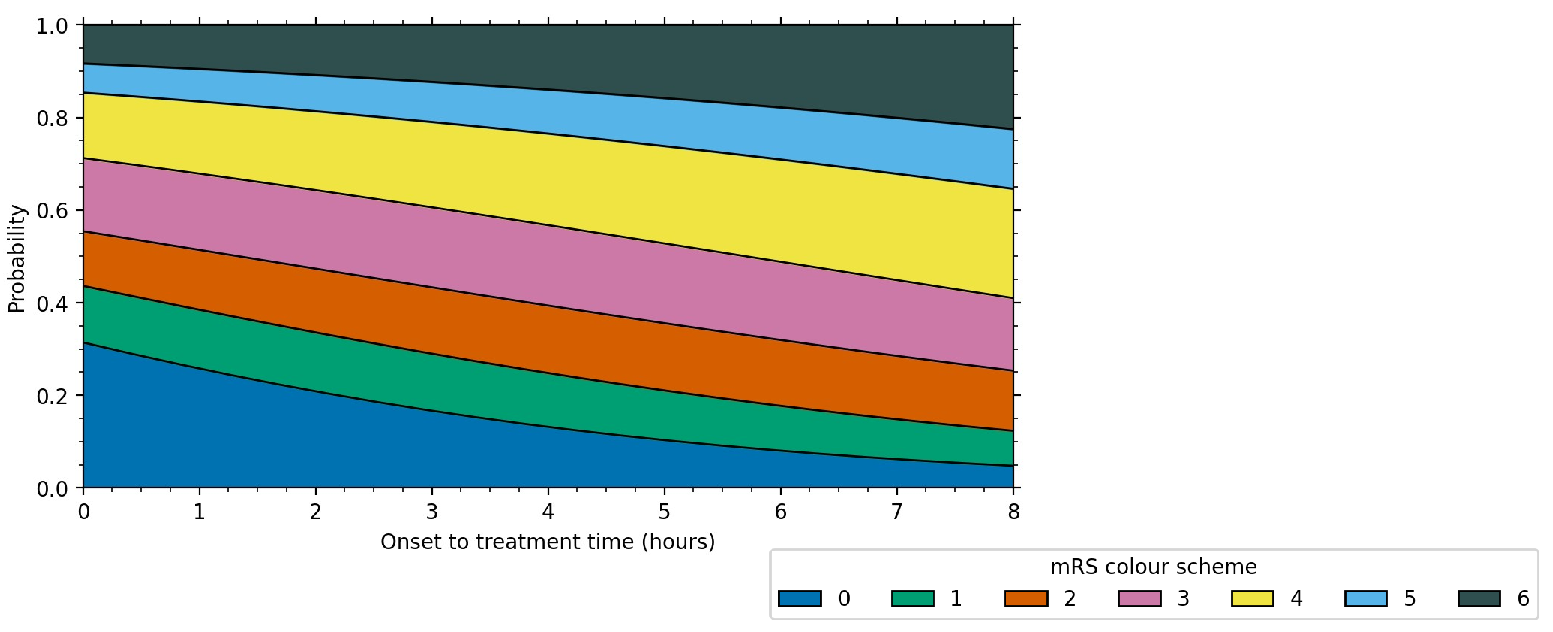
\includegraphics[width=\textwidth]{./images/probs_with_time_not_annotated}
\end{center} 


% Calculate how they vary with time from some assumption (straight line in log(odds ratio) goes to these curvy exponential-esque logistic functions. 

% Basic idea of take someone in mRS=2, draw line horizontally to the treatment time, then see expected mRS bin at that time. 

The variation with time is a logistic function. 
% Leave in phantom text so that this slide and the next have the figure at the same vertical alignment:
\phantom{If treated at time 3h30min, Patient X will see an improvement in mRS score of 1 c.}

\vspace{1em}
\smallurl{http://localhost:8888/lab/tree/stroke_outcome/mRS_outcomes_maths.ipynb}

\end{frame}


%%%%%%%%%%%%%%%%%%%%%%%%%%%%%%%%%%%%%%%%%%%%%%%%%%%%%%%%%%%%%%%

\begin{frame}
\frametitle{Outcome variation with time}

Expected outcomes of patients with large-vessel occlusions treated with thrombectomy: 

\begin{center} 
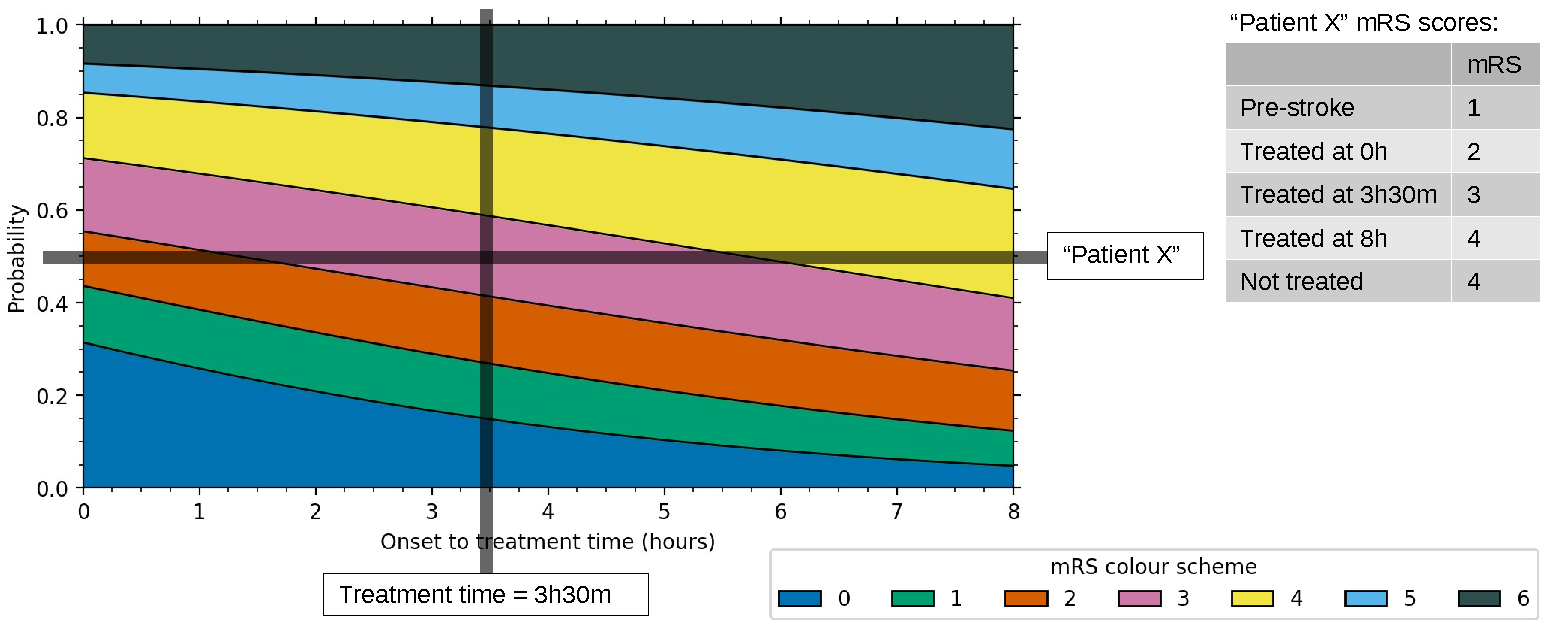
\includegraphics[width=\textwidth]{./images/probs_with_time_annotated}
\end{center} 

% Basic idea of take someone in mRS=2, draw line horizontally to the treatment time, then see expected mRS bin at that time. 

If treated at time 3h30min, Patient X will see an improvement in mRS score of 1 compared with receiving no treatment. 

\vspace{1em}
\smallurl{http://localhost:8888/lab/tree/stroke_outcome/mRS_outcomes_maths.ipynb}


\end{frame}

%%%%%%%%%%%%%%%%%%%%%%%%%%%%%%%%%%%%%%%%%%%%%%%%%%%%%%%%%%%%%%%


\begin{frame}
\frametitle{Patient population}

\begin{center} 
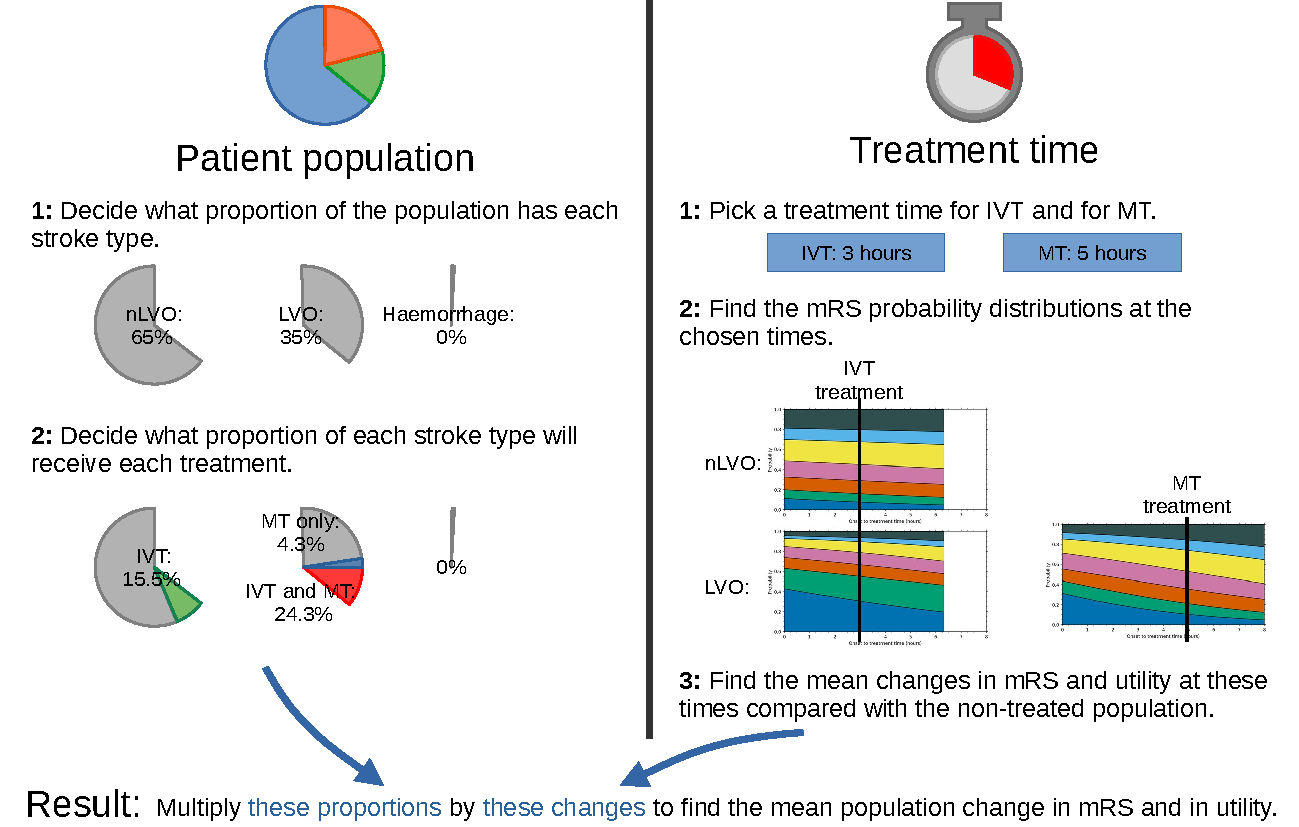
\includegraphics[width=\textwidth]{./images/population_method}
\end{center} 

\end{frame}


%%%%%%%%%%%%%%%%%%%%%%%%%%%%%%%%%%%%%%%%%%%%%%%%%%%%%%%%%%%%%%%

\subsection{Streamlit app} % Printed on outline slide. 
\begin{frame}
\frametitle{Streamlit app}

\textbf{To do - finish this slide} 

Streamlit app: ADD LINK HERE 


\begin{columns}
    \column{0.5\textwidth}
    GitHub repository: 
    \begin{center} 
    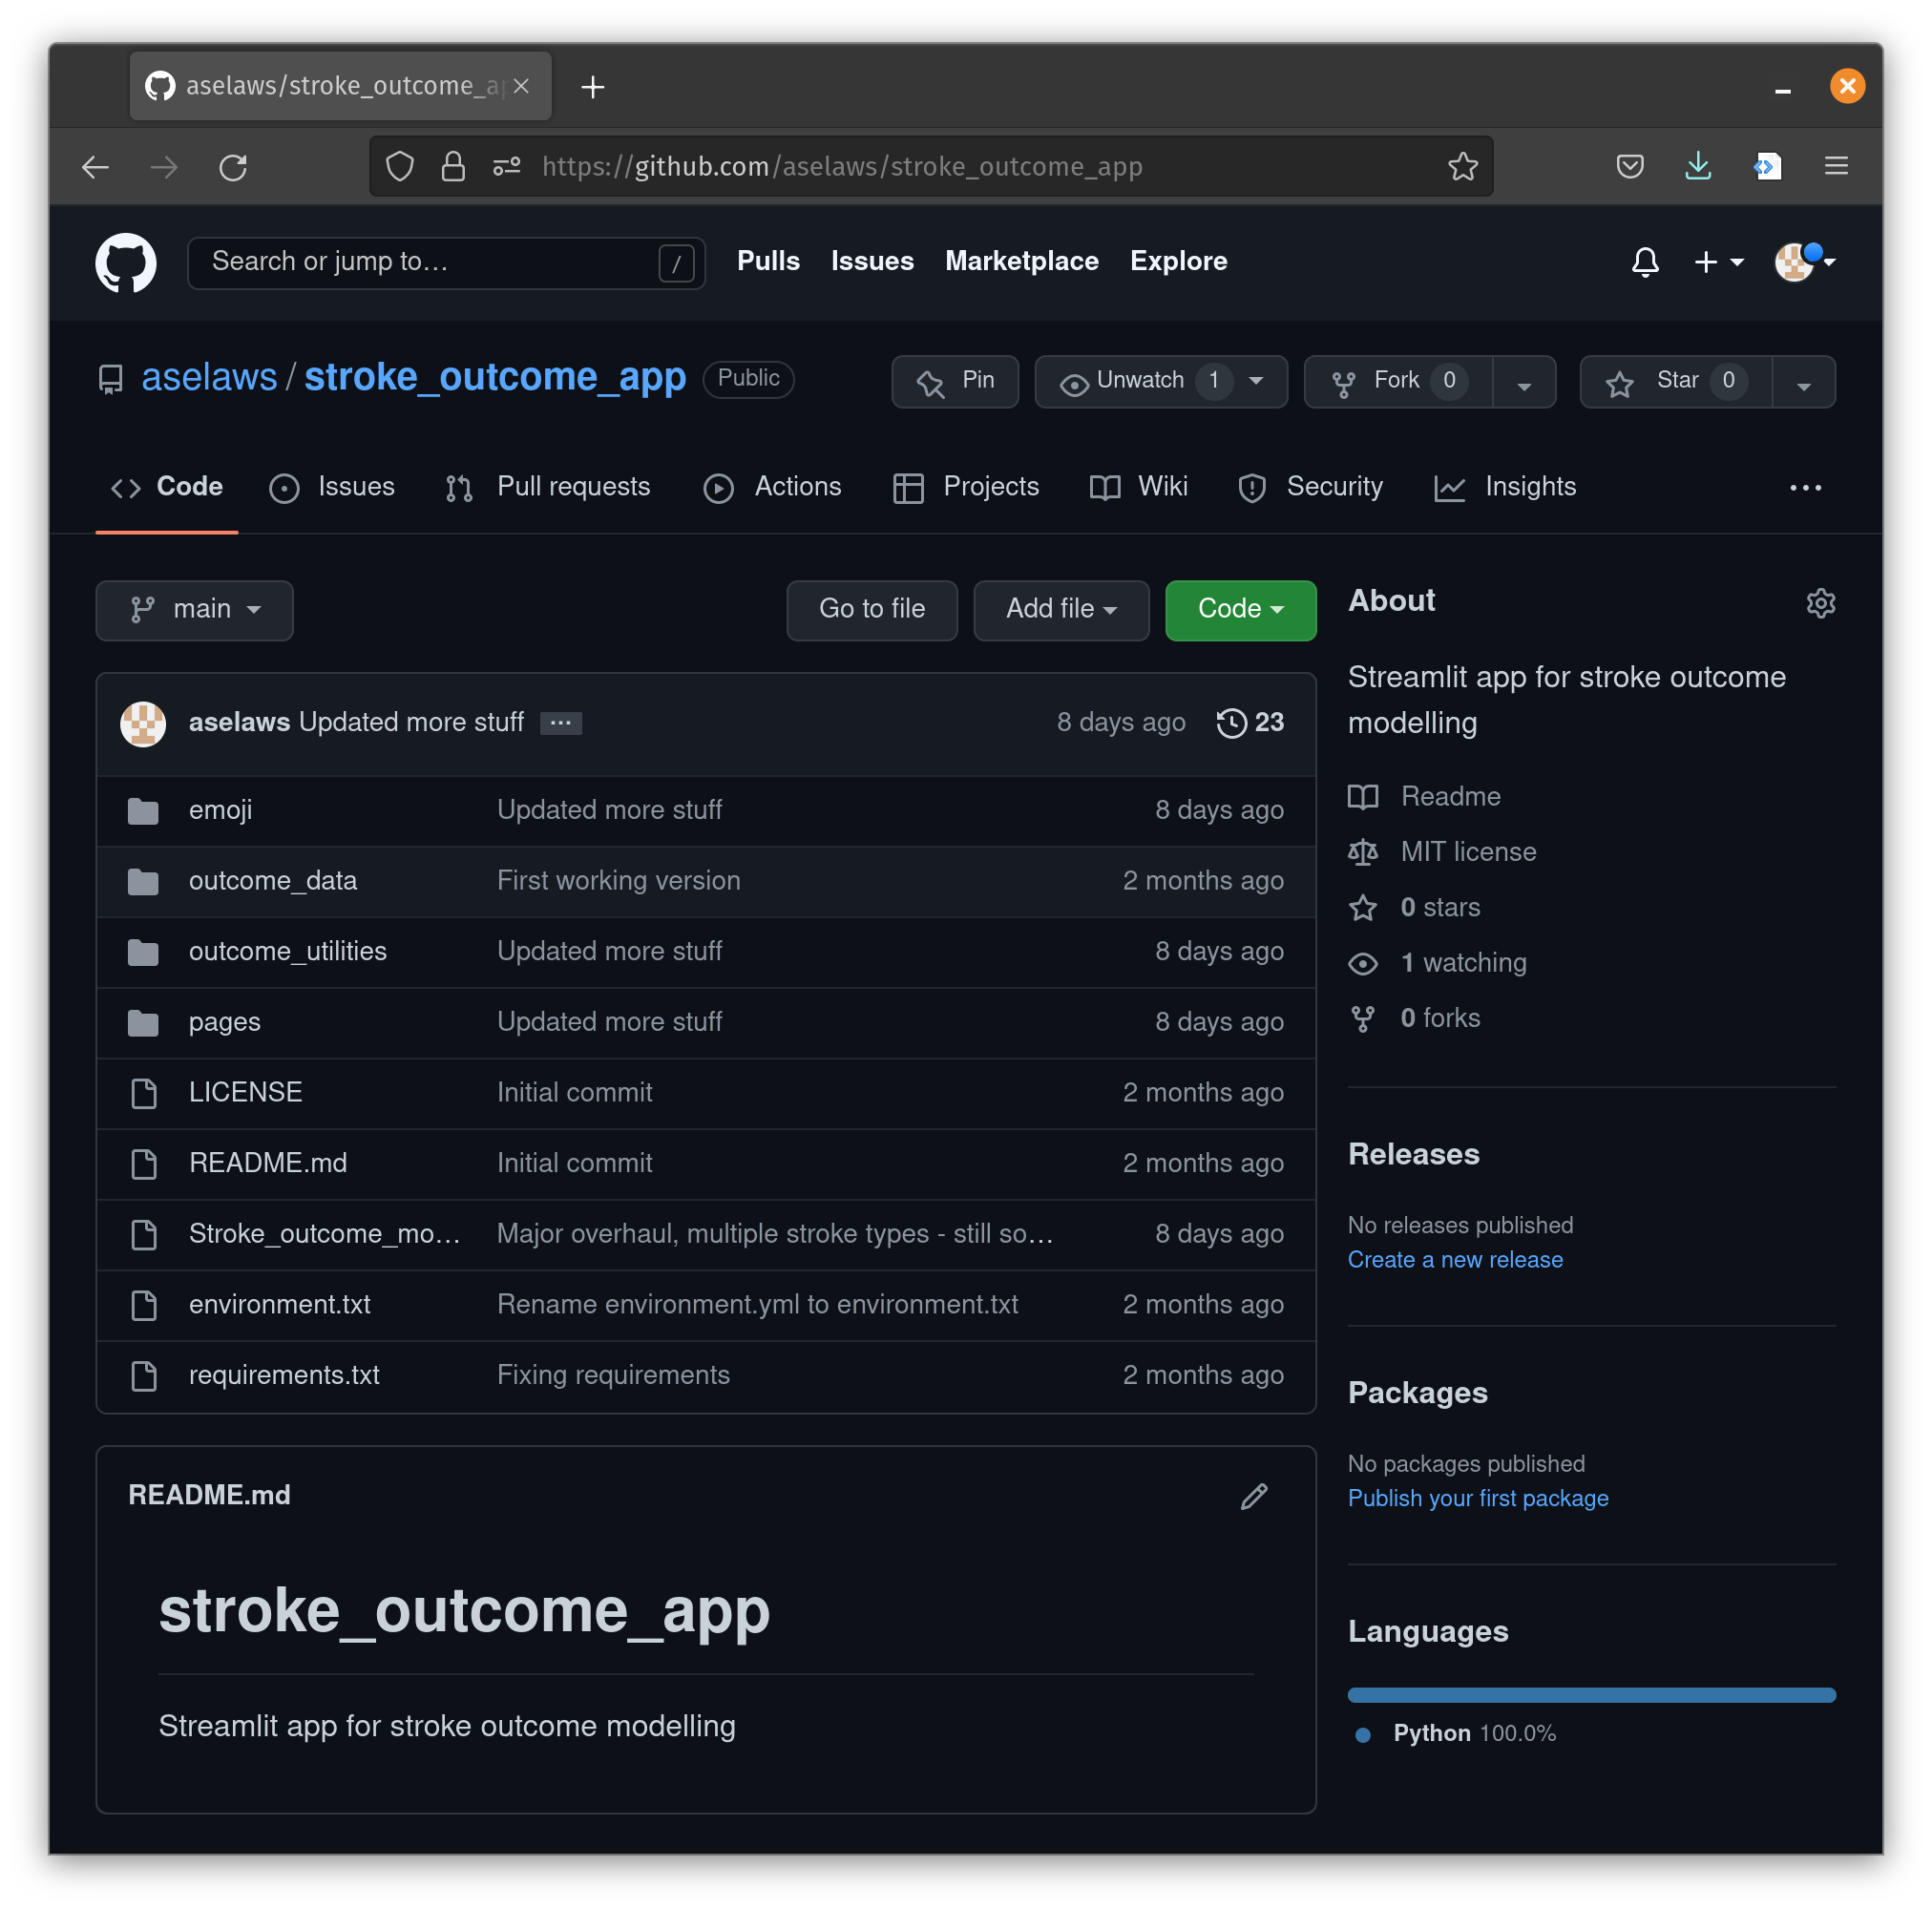
\includegraphics[width=0.5\textwidth]{./images/GitHub-streamlit}
    \end{center} 
  
    \column{0.5\textwidth}
    Streamlit app:
    \begin{center} 
    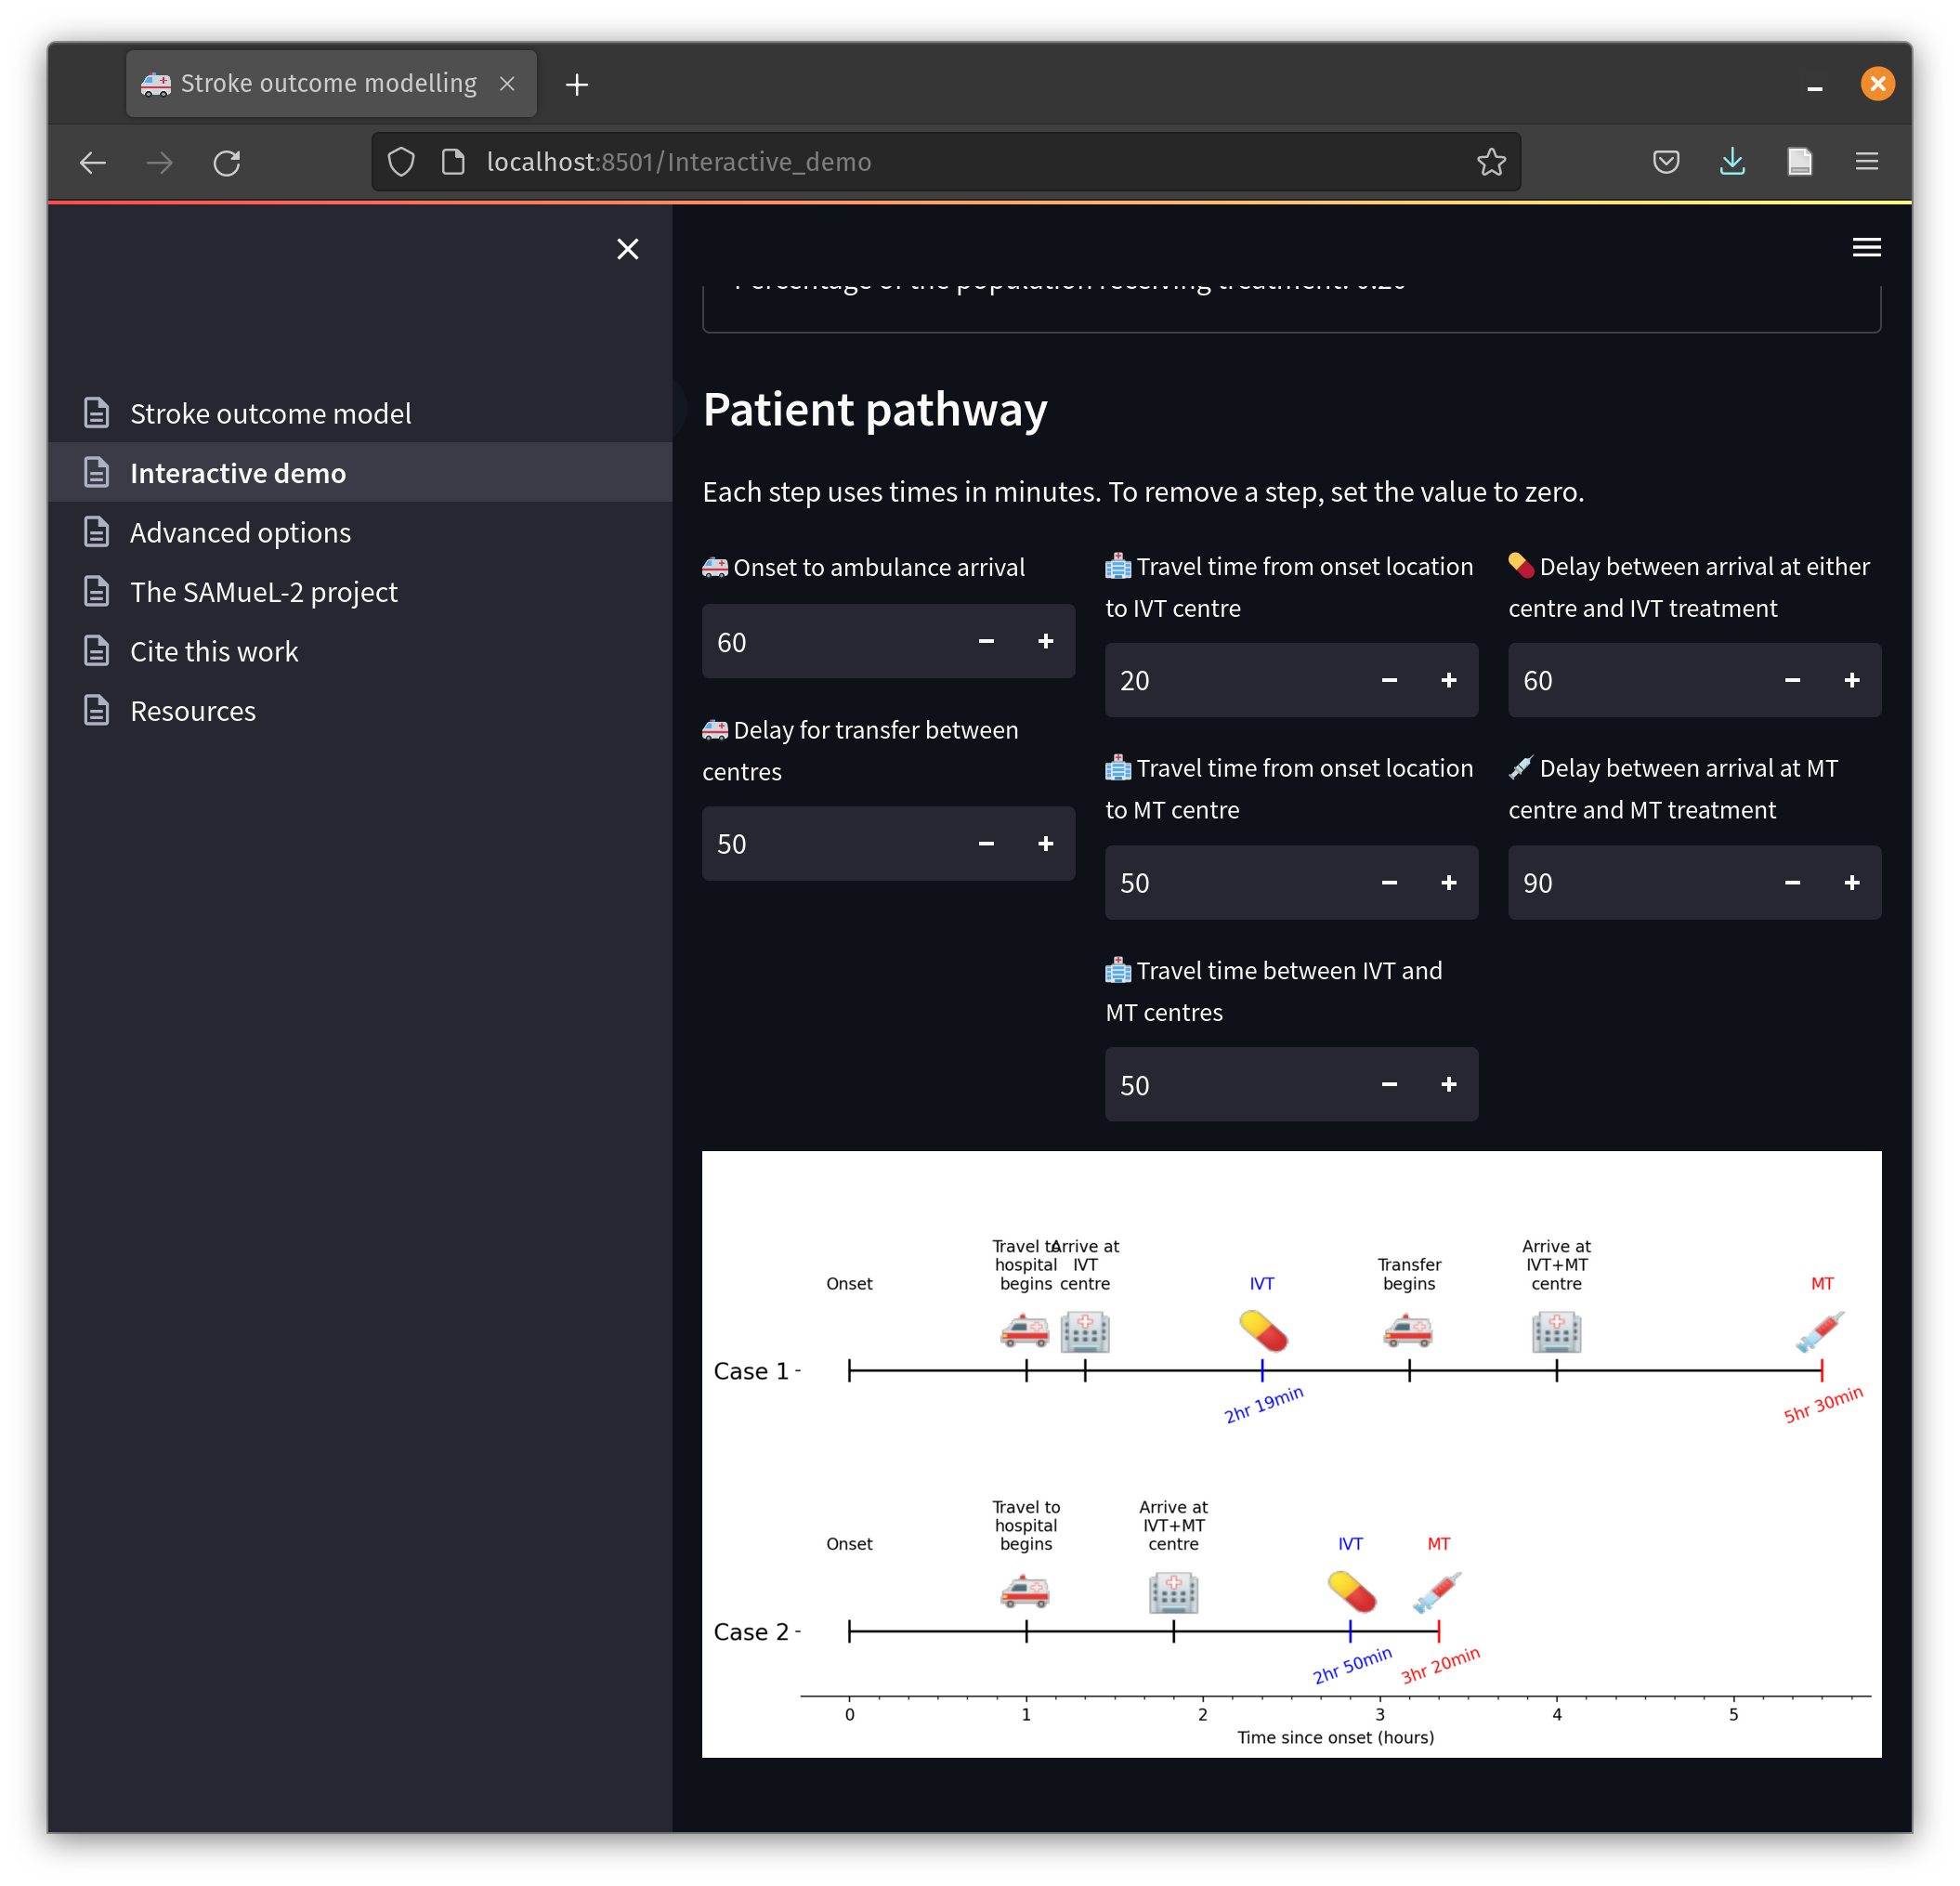
\includegraphics[width=0.5\textwidth]{./images/Streamlit-screenshot}
    \end{center} 
    (placeholder - get day mode) 
\end{columns}

Linked to this (messy!) GitHub repository: \smallurl{https://github.com/aselaws/stroke_outcome_app}

\end{frame}


%%%%%%%%%%%%%%%%%%%%%%%%%%%%%%%%%%%%%%%%%%%%%%%%%%%%%%%%%%%%%%%
\begin{frame}{Thank you!!}
    Thank you for your time and attention!
\end{frame}

%%%%%%%%%%%%%%%%%%%%%%%%%%%%%%%%%%%%%%%%%%%%%%%%%%%%%%%%%%%%%%%


% EXTRA SLIDE(S)

\begin{frame}[noframenumbering]{Reserve slides}
    
\end{frame}


%%%%%%%%%%%%%%%%%%%%%%%%%%%%%%%%%%%%%%%%%%%%%%%%%%%%%%%%%%%%%%%

\begin{frame}[noframenumbering]
\frametitle{Applying our models at hospital level}

\begin{center}
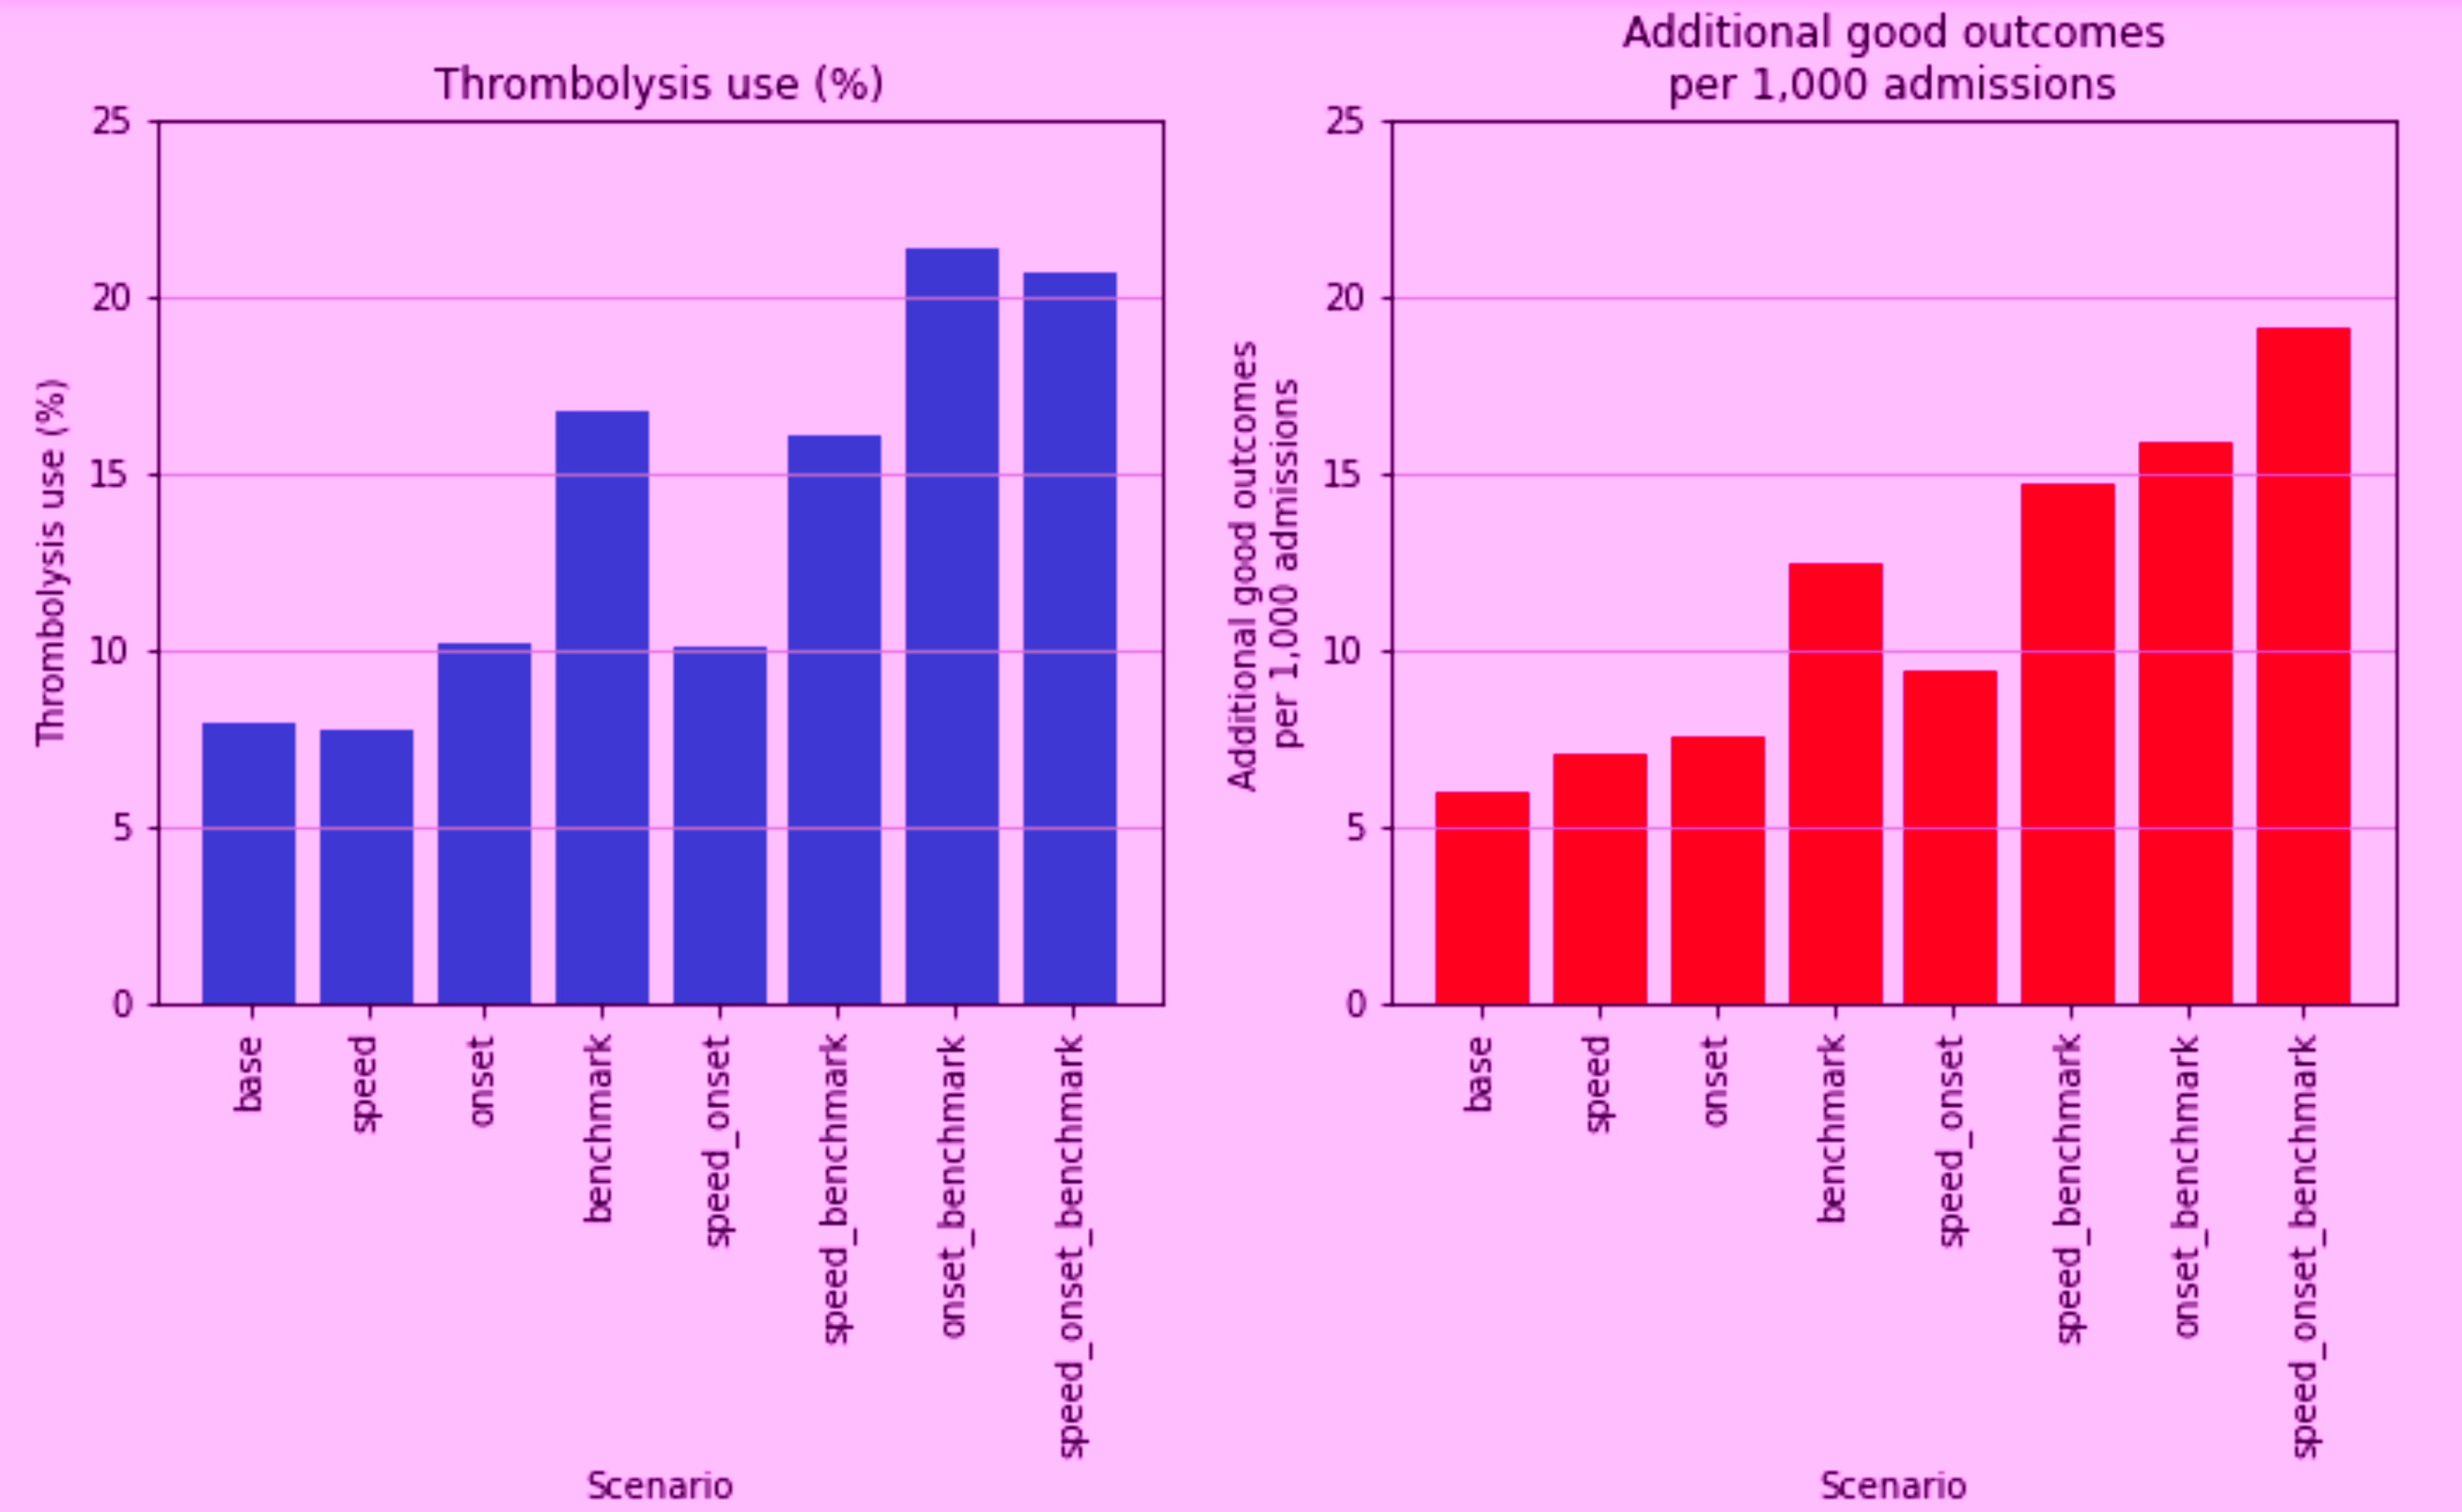
\includegraphics[width=0.95\textwidth]{./images_pink/hosp_scenario_1}
\end{center}

\end{frame}


%%%%%%%%%%%%%%%%%%%%%%%%%%%%%%%%%%%%%%%%%%%%%%%%%%%%%%%%%%%%%%%

\begin{frame}[noframenumbering]
\frametitle{mRS variation with time}

\begin{center} 
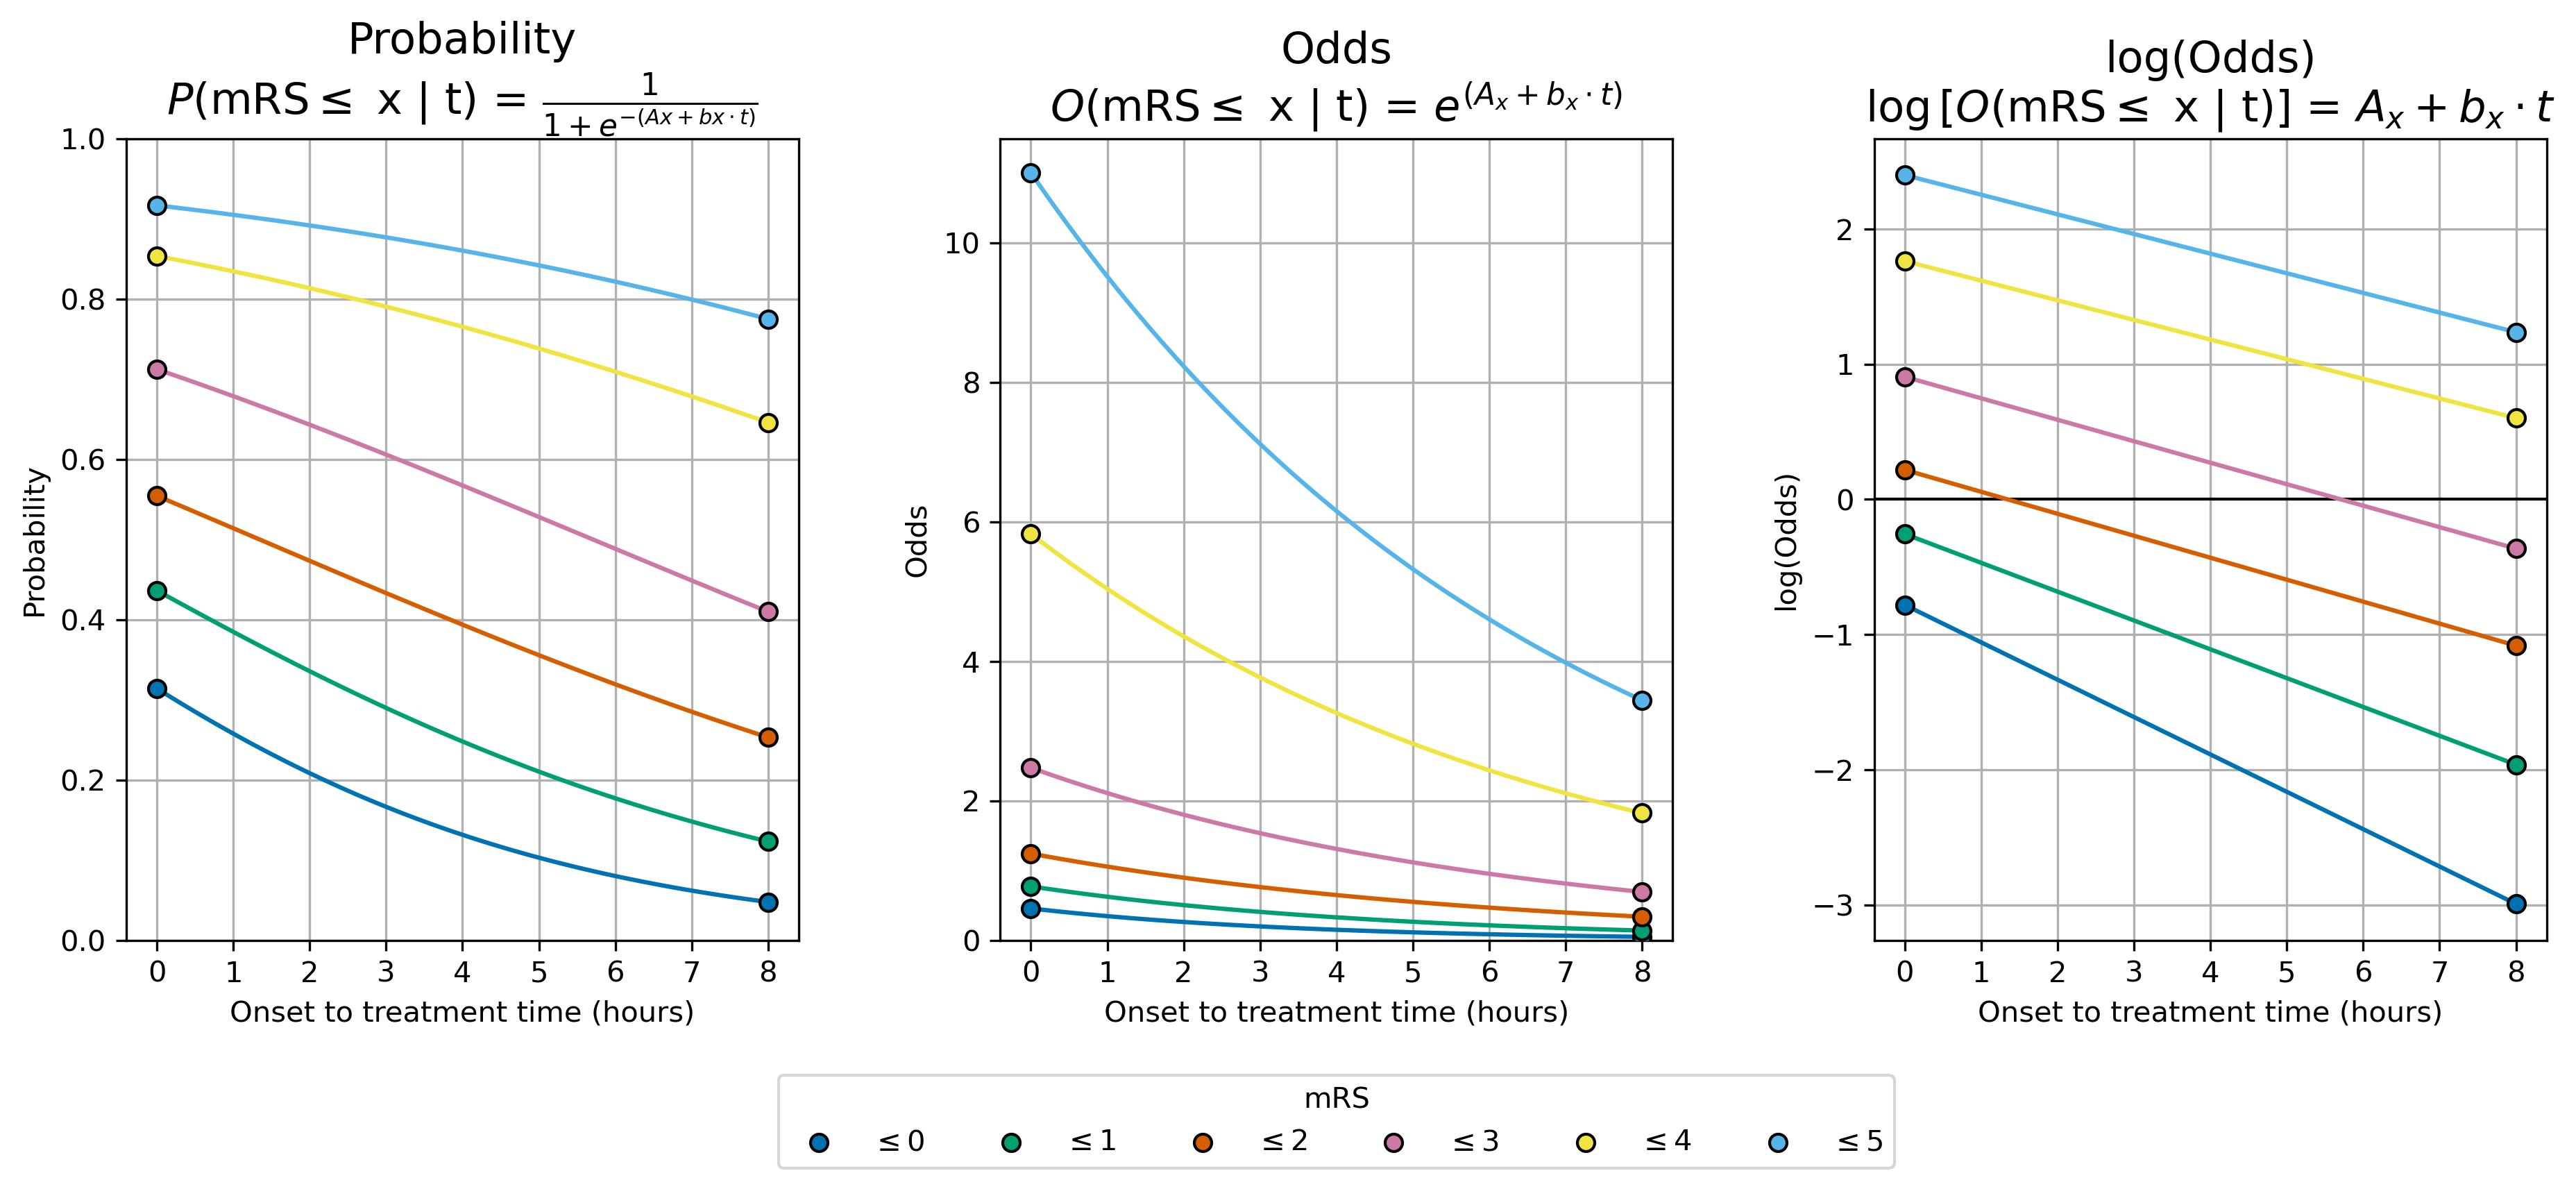
\includegraphics[width=\textwidth]{./images/time_varying_probs_odds_logodds}
\end{center} 

\vspace{1em}
\smallurl{http://localhost:8888/lab/tree/stroke_outcome/mRS_outcomes_maths.ipynb}

\end{frame}


%%%%%%%%%%%%%%%%%%%%%%%%%%%%%%%%%%%%%%%%%%%%%%%%%%%%%%%%%%%%%%%


\begin{frame}[noframenumbering]
\frametitle{Variation with time for different stroke types and treatment types.}

\begin{columns}
    \footnotesize
    \column{0.5\textwidth}
    nLVO treated with IVT 
    \begin{center} 
    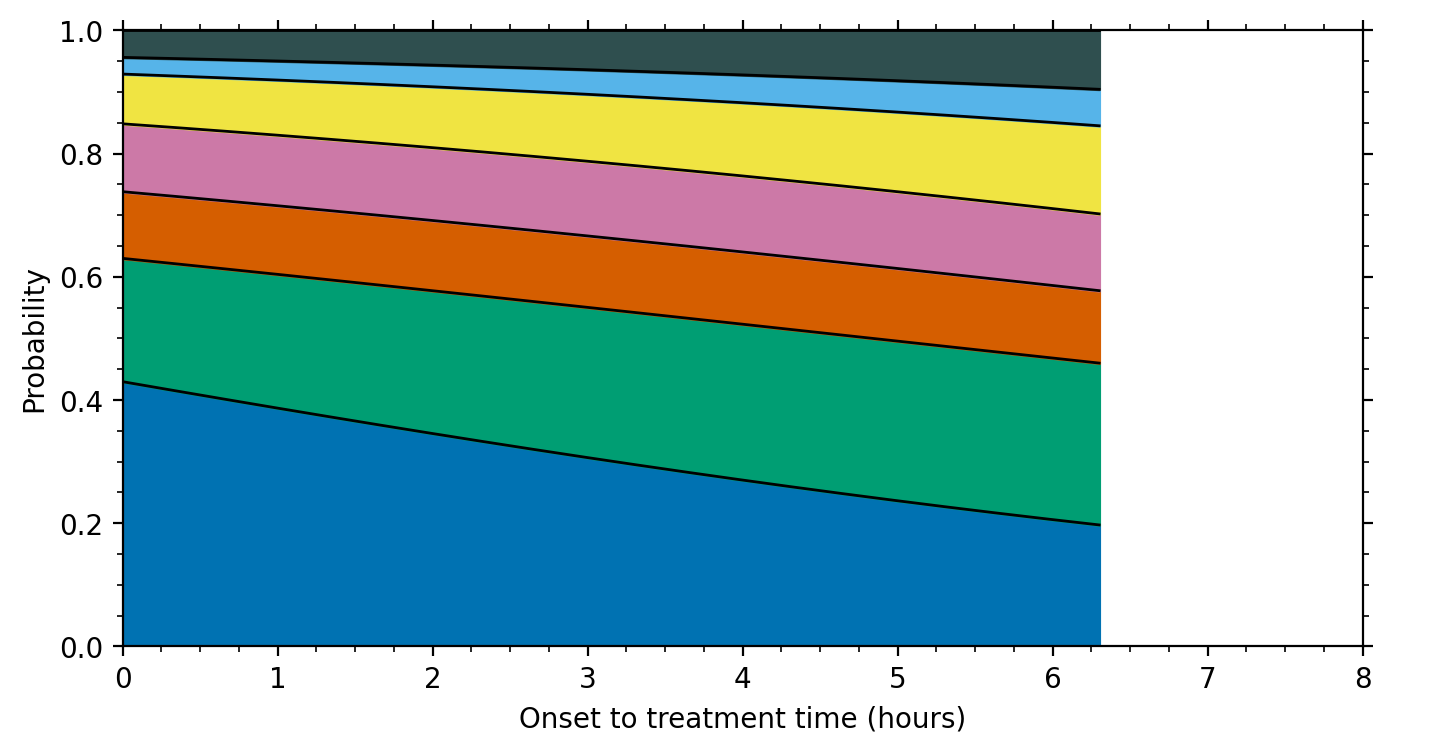
\includegraphics[width=\textwidth]{./images/probs_with_time_nlvo_ivt}
    \end{center} 
    %
    \vspace{1em}
    \smallurl{http://localhost:8888/lab/tree/stroke_outcome/mRS_outcomes_maths.ipynb}

    \column{0.5\textwidth}
    LVO treated with IVT
    \begin{center} 
    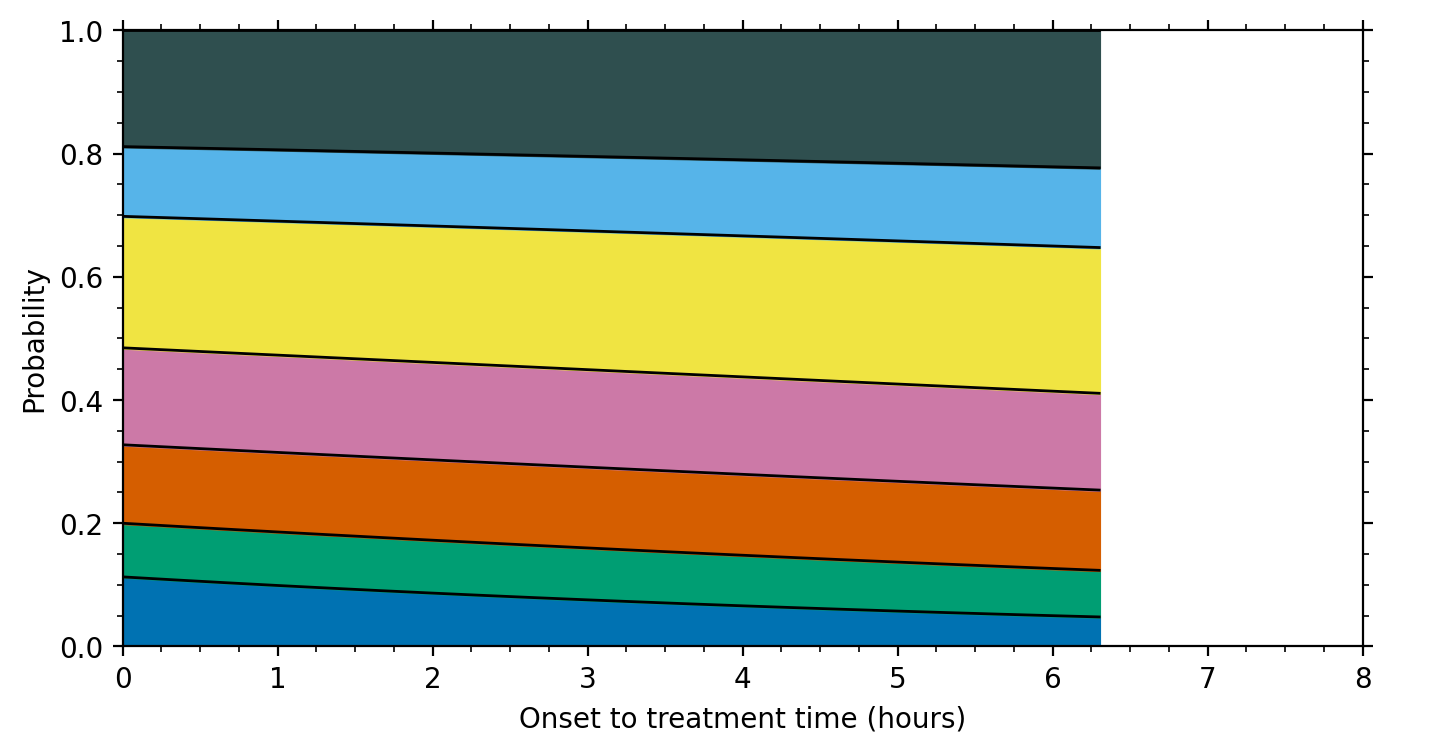
\includegraphics[width=\textwidth]{./images/probs_with_time_lvo_ivt}
    \end{center} 
    %
    LVO treated with MT 
    \begin{center} 
    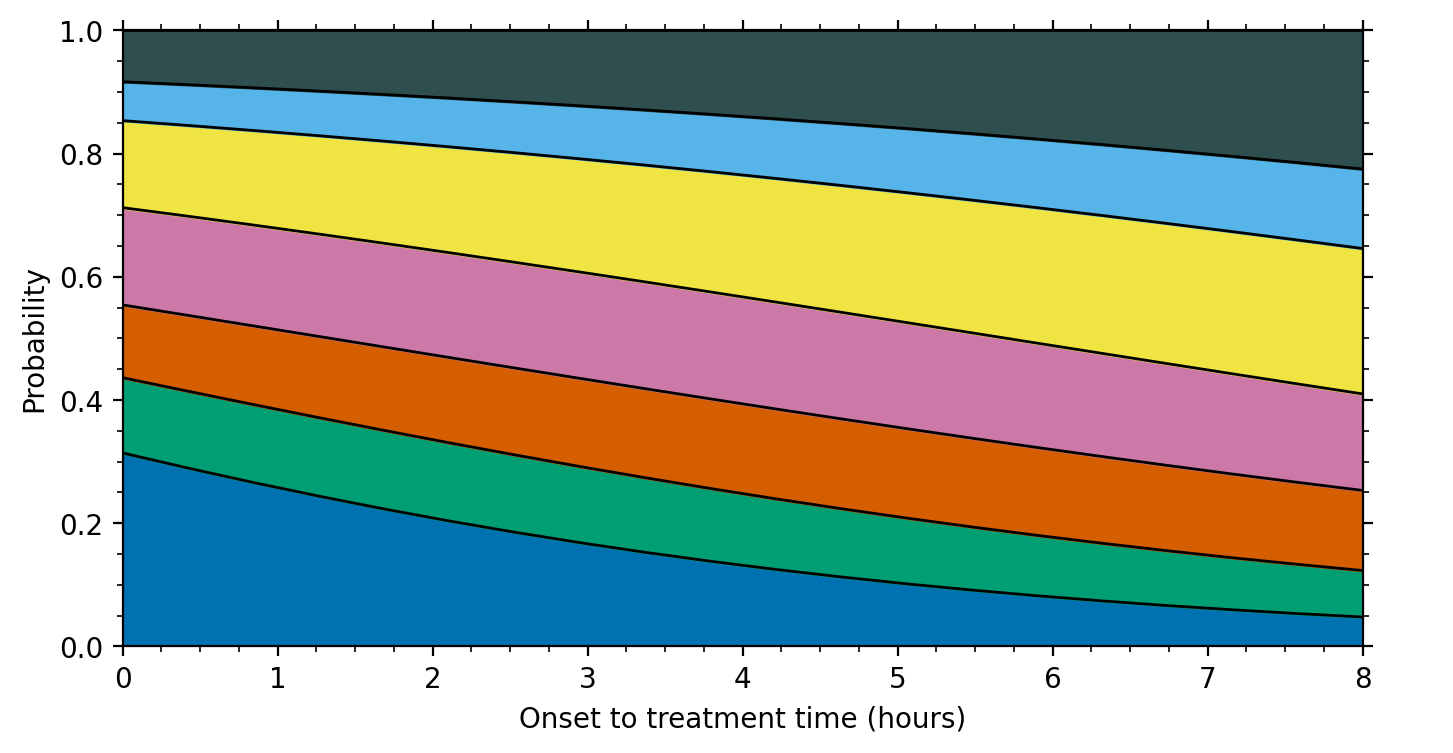
\includegraphics[width=\textwidth]{./images/probs_with_time_lvo_mt}
    \end{center} 
    %
\end{columns}



\end{frame}


%%%%%%%%%%%%%%%%%%%%%%%%%%%%%%%%%%%%%%%%%%%%%%%%%%%%%%%%%%%%%%%



\begin{frame}[noframenumbering]
\frametitle{Basic geography with stroke outcome modelling}

\footnotesize{What difference does it make if everyone in the patient population:}
\begin{enumerate}
    \footnotesize
    \item travels to an IVT-only centre, and then transfers to a combined IVT+MT centre? 
    \item travels directly to a combined IVT+MT treatment centre? 
\end{enumerate} 

\footnotesize{For the case when the centres are 90 minutes apart and travel begins 90 minutes after the stroke onset:}

\begin{center}
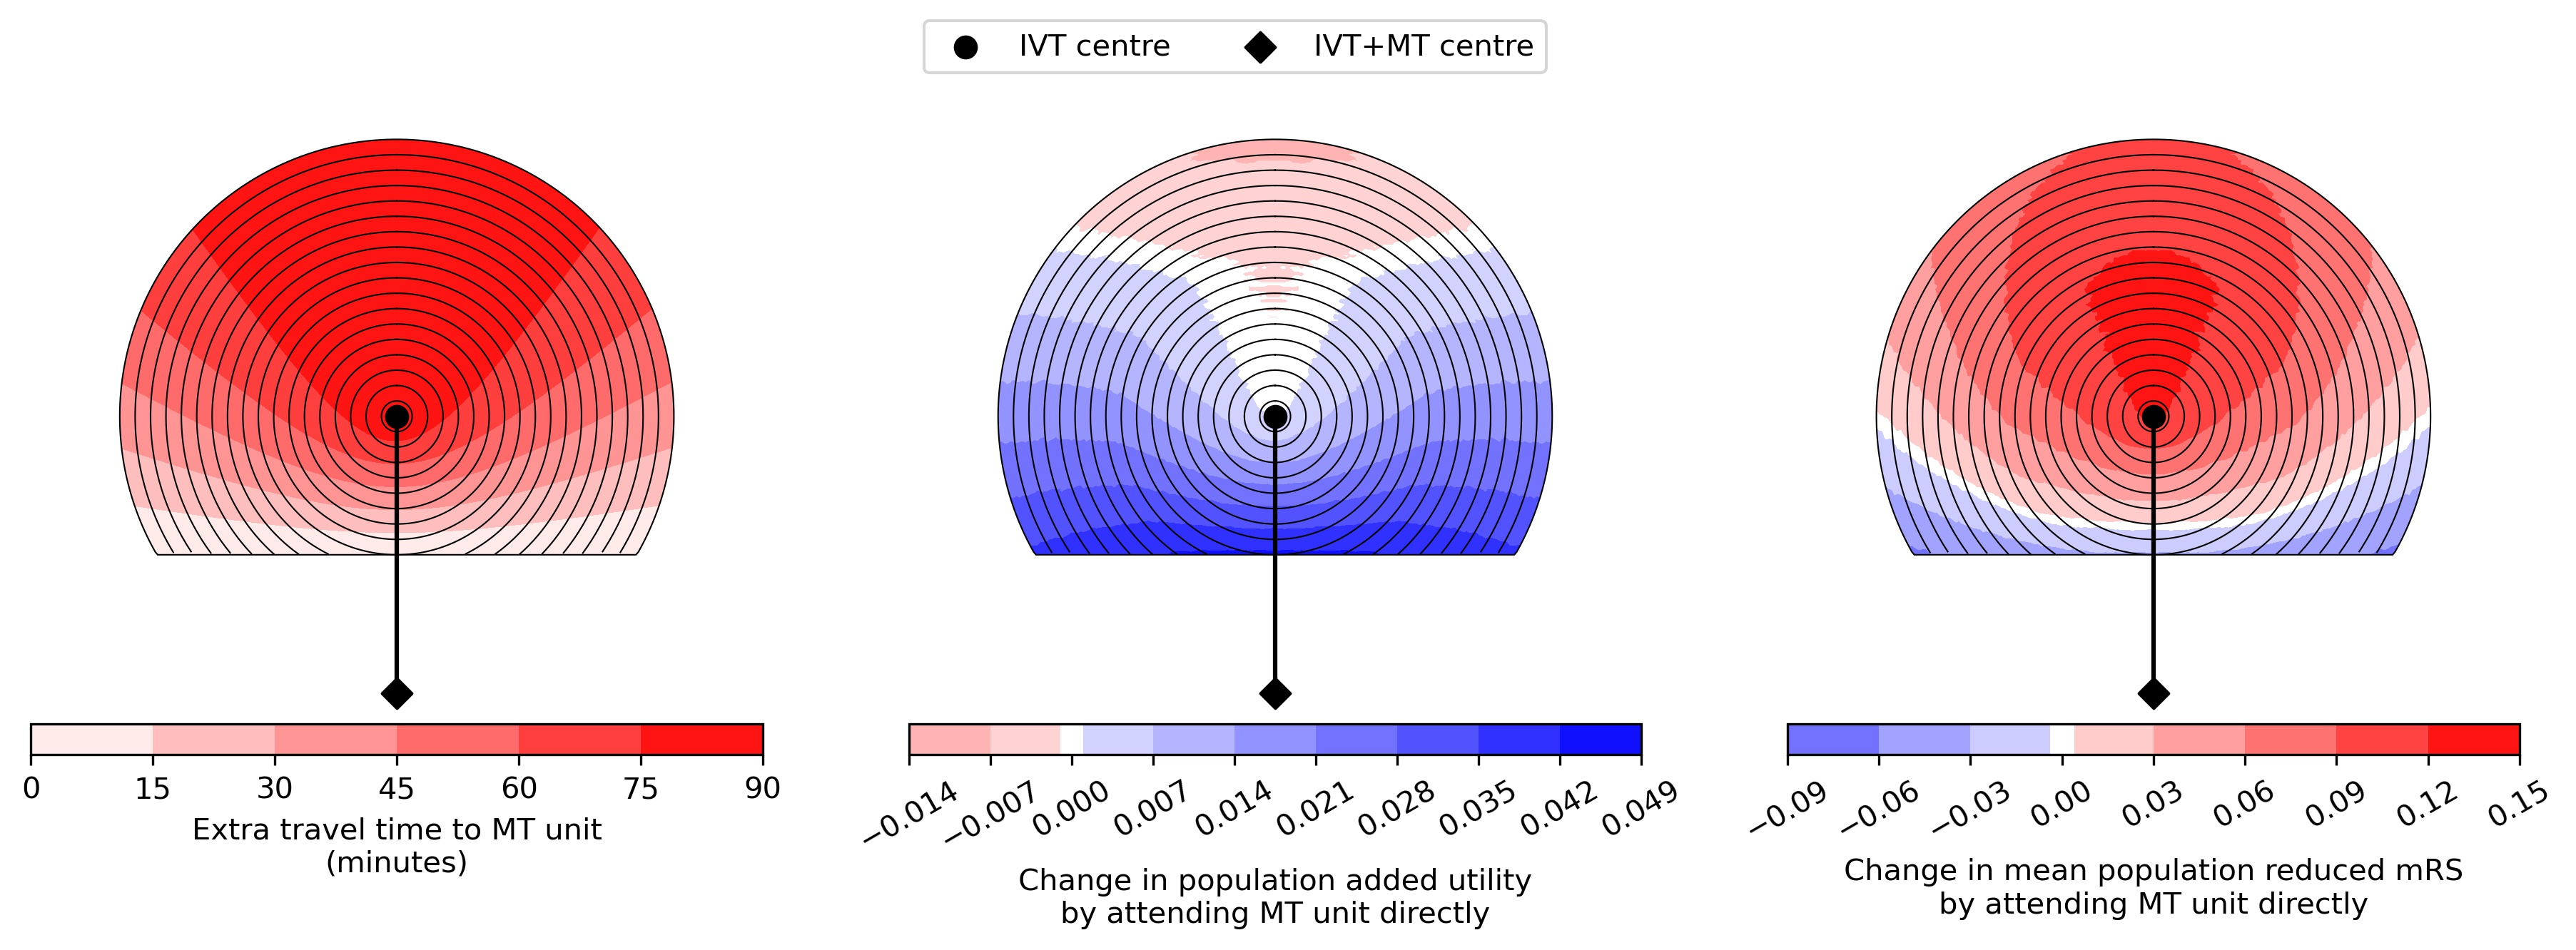
\includegraphics[width=\textwidth]{./images/circle_plots_t-IVT-to-MT=90_t-onset-to-ambo=90}
\end{center} 

% Basically a direct comparison of lots of different locations

% Assume everyone travels in a straight line, no hills or anything slowing them down. 

% Generally interesting, can use the same idea to apply to actual geography. 

\footnotesize{\emph{These are early results and could change.} There is a large difference in which locations have zero gain depending on the outcome measure.}

\vspace{0.5em}
\tiny{Based on similar geographic modelling by Holodinsky et al. 2018.}

\smallurl{https://github.com/samuel-book/stroke_outcome/blob/main/geography.ipynb}

\end{frame}


%%%%%%%%%%%%%%%%%%%%%%%%%%%%%%%%%%%%%%%%%%%%%%%%%%%%%%%%%%%%%%%

\end{document}
